% =============================================================================
%  Witten《Quantum Field Theory and the Jones Polynomial》中文译注本
%  Commun. Math. Phys. 121 (1989) 351–399
%  编译：在 witten1989 目录下运行  xelatex main.tex  两遍
% =============================================================================
% =============================================================================
%  Witten《Quantum Field Theory and the Jones Polynomial》
%  （Commun. Math. Phys. 121 (1989) 351–399）中文译注本 —— 导言区
%  编译：xelatex（两遍）；中文字体：fandol（TeX Live 自带）
% =============================================================================
\documentclass[11pt,a4paper]{article}

\usepackage[UTF8, fontset=fandol, heading=true]{ctex}
\usepackage{amsmath}
\usepackage{amssymb}
\usepackage{mathtools}
\usepackage{bm}
\usepackage[a4paper,left=2.5cm,right=2.5cm,top=2.6cm,bottom=2.6cm]{geometry}
\usepackage{graphicx}
\usepackage{xcolor}
\usepackage{tcolorbox}
\tcbuselibrary{breakable, skins}
\usepackage{enumitem}
\usepackage{booktabs}
\usepackage{array}
\usepackage[font=small,labelfont=bf,labelsep=quad]{caption}
\usepackage[colorlinks=true,
            linkcolor=blue!45!black,
            citecolor=blue!45!black,
            urlcolor=blue!45!black]{hyperref}

\linespread{1.12}
\setlength{\emergencystretch}{3em}
\allowdisplaybreaks[3]

\graphicspath{{figures/}}

\renewcommand{\figurename}{图}
\renewcommand{\tablename}{表}
\renewcommand{\refname}{参考文献}
\renewcommand{\contentsname}{目录}
\renewcommand{\abstractname}{摘要}

\hypersetup{
  pdftitle={量子场论与 Jones 多项式（Witten 1989 中文译注本）},
  pdfauthor={Edward Witten（原著）；中文译注：DeepSeek Harness},
  pdfsubject={Chern-Simons theory, Jones polynomial, topological quantum field theory},
  pdfkeywords={Chern-Simons, Jones polynomial, knot invariant, conformal field theory, 3-manifolds},
  bookmarksnumbered=true
}

% ---------------------------------------------------------------------------
%  常用记号（仅导言区定义，正文片段中不要另造宏）
% ---------------------------------------------------------------------------
\DeclareMathOperator{\Tr}{Tr}
\DeclareMathOperator{\sgn}{sgn}
\newcommand{\dd}{\mathrm{d}}
\newcommand{\figdir}{figures}

% ---------------------------------------------------------------------------
%  「本节重点」：蓝色方框，编译后可见
% ---------------------------------------------------------------------------
\newenvironment{keypoints}{%
    \par\medskip
    \begin{tcolorbox}[enhanced, breakable,
        colback=blue!4!white, colframe=blue!40!black,
        boxrule=0.5pt, arc=2pt, left=6pt, right=6pt, top=4pt, bottom=4pt,
        title={\small\textbf{本节重点}\quad{\footnotesize（译者所加，非原文内容）}},
        fonttitle=\bfseries, coltitle=black, colbacktitle=blue!10!white,
        toptitle=1pt, bottomtitle=1pt]
    \begin{itemize}[leftmargin=1.4em, itemsep=2pt, topsep=2pt, parsep=0pt]
}{%
    \end{itemize}
    \end{tcolorbox}
    \par\medskip
}

% ---------------------------------------------------------------------------
%  「译注」：橙色方框，编译后可见（用于少量需要读者当场看到的说明）
%  绝大多数批注应写成 LaTeX 注释行 % [Tutor Note: ...]，不占用版面。
% ---------------------------------------------------------------------------
\newcounter{yizhu}
\newenvironment{yizhu}[1][]{%
    \par\medskip
    \refstepcounter{yizhu}%
    \begin{tcolorbox}[enhanced, breakable,
        colback=orange!4!white, colframe=orange!60!black,
        boxrule=0.5pt, arc=2pt, left=6pt, right=6pt, top=4pt, bottom=4pt,
        title={\small\textbf{译注 \theyizhu\if\relax\detokenize{#1}\relax\else\ ——#1\fi}},
        fonttitle=\bfseries, coltitle=black, colbacktitle=orange!12!white,
        toptitle=1pt, bottomtitle=1pt]
}{%
    \end{tcolorbox}
    \par\medskip
}

\begin{document}

\title{\bfseries 量子场论与 Jones 多项式\\[6pt]
       \large\normalfont Quantum Field Theory and the Jones Polynomial}
\author{Edward Witten\\
        {\small School of Natural Sciences, Institute for Advanced Study,
        Olden Lane, Princeton, NJ 08540, USA}\\[4pt]
        {\small 中文译注：DeepSeek Harness}}
\date{Commun.\ Math.\ Phys.\ \textbf{121} (1989) 351--399（收稿 1988 年）}
\maketitle

\begin{abstract}
本文证明：2+1 维量子杨–米尔斯理论，当其作用量纯粹由陈–西蒙斯项构成时，是可精确求解的，
并为以三维方式理解纽结理论中的 Jones 多项式提供了自然的框架。在这一版本中，
Jones 多项式可以从 $S^3$ 推广到任意三维流形，从而给出可由手术表示计算的三维流形不变量。
这些结果为 $1+1$ 维共形场论带来了出人意料的新启示。
\end{abstract}

\begin{tcolorbox}[enhanced, breakable, colback=gray!3!white, colframe=gray!55!black,
    boxrule=0.5pt, arc=2pt, left=8pt, right=8pt, top=5pt, bottom=5pt,
    title={\small\textbf{译者说明}}, fonttitle=\bfseries,
    coltitle=black, colbacktitle=gray!12!white, toptitle=1pt, bottomtitle=1pt]
\small
\begin{itemize}[leftmargin=1.2em, itemsep=2pt, topsep=0pt, parsep=0pt]
  \item \textbf{底本。}Edward Witten，\emph{Quantum Field Theory and the Jones Polynomial}，
        \emph{Commun.\ Math.\ Phys.}\ \textbf{121} (1989) 351--399（49 页扫描件）。
        译文页边所注“原文 p.~$n$”均为该刊印刷页码，对应 PDF 页号 $n-350$。
  \item \textbf{公式编号。}完全沿用原文编号（式 (1.1)、(2.14)……），不重排、不跳号；
        正文以“式 (2.14)”形式引用。原文脚注以 \LaTeX{} 脚注形式保留。
  \item \textbf{批注约定。}凡标以 \texttt{\% [Tutor Note: ...]} 的 LaTeX 注释行，均为译者所加，
        编译后不显示；内容为易错点预警、作者跳过的论证环节说明、原文笔误指正与术语考订。
        每节开头的“本节重点”方框亦为译者所加。
  \item \textbf{译名。}采用中文学术界约定：gauge theory 译“规范理论”，Chern--Simons 译
        “陈–西蒙斯”，holonomy 译“和乐”（holonomy），anomaly 译“反常”，
        knot/link 译“纽结/链环”，framing 译“标架（framing）”。
        人名与理论专名（Jones、Kauffman、Witten、Verlinde 等）保留原文。
  \item \textbf{原文保留。}$S^3$、$S^2\times S^1$ 等符号、文献引用编号 $[n]$ 与原文一致，
        便于对照原刊；参考文献表照原文顺序与编号排印，未作增补。
\end{itemize}
\end{tcolorbox}

\tableofcontents
\newpage


% =============================================================================
%  s00-front.tex —— 引言（原文 PDF p.1–2 及 p.3 开头；印刷页 351–353）
%  原文此处无节标题，为便于阅读由译者加不编号标题「引言」。
% =============================================================================
\section*{引言}
\markboth{引言}{引言}
\addcontentsline{toc}{section}{引言（原文无标题）}

\begin{keypoints}
    \item \textbf{物理图像：}存在一类量子场论，其可观测量全为拓扑不变量；但“广义协变”不必通过
          对度规积分来实现，只要拉格朗日量本身不含度规即可。本文要构造的正是这样一个理论。
    \item \textbf{数学工具：}三维流形上的陈–西蒙斯作用量；相交形式、同调群、模空间等拓扑与几何工具。
    \item \textbf{关键结论：}Atiyah 提出的两个问题中，Donaldson 理论的物理解释已在 [4] 中给出；
          本文解决第二个问题——为 Jones 多项式给出内蕴三维的量子场论定义。
\end{keypoints}

在去年 Hermann Weyl 讨论会的一次演讲中 [1]，Michael Atiyah 向量子场论学家提出了两个问题。
第一个问题是为 Donaldson 理论给出物理解释；第二个问题是为纽结理论中的 Jones 多项式
寻找一个内蕴的三维定义。这两个问题大致可以这样描述。

Donaldson 理论是理解四维几何的关键。至少从宏观上看，四维正是物理的维度，
因此不妨稍作引申地说：Donaldson 理论是理解时空几何的关键。几何学家早已知道
（通过 de Rham 理论），自对偶与反自对偶的麦克斯韦方程与四维流形的自然拓扑不变量
——即第二同调群及其相交形式——相联系。对于单连通四维流形，这些本质上就是全部经典不变量，
但它们仍使许多基本问题无法回答。Donaldson 的洞见 [2] 在于认识到，
自对偶杨–米尔斯方程解空间的模空间可以成为处理这些问题的有力工具。

% [Tutor Note: 易错点] 此处“第二同调群及其相交形式”是就单连通闭四维流形而言：$H_2(M;\mathbb{Z})$
% 配上对称双线性型 $Q(\alpha,\beta)=\langle\alpha\smile\beta,[M]\rangle$，由 Poincaré 对偶与
% de Rham 上同调的自对偶/反自对偶分解给出。原文说“自对偶与反自对偶的麦克斯韦方程”与此相关，
% 指的是 $H^2$ 上 Hodge $\star$ 的本征分解（$\star^2=1$ 在四维中间次数上），而不是说经典麦克斯韦
% 方程的解集本身是同调群；读后面 Donaldson 理论部分时要记住这条对应。
%
% [Tutor Note: 含糊点] 原文说“这些本质上就是全部经典不变量”，依据的是 Freedman 关于单连通
% 闭拓扑四维流形的分类定理：这类流形由相交形式的同构类（秩、符号差、奇偶性等不变量）
% 连同 Kirby–Siebenmann 不变量（光滑化障碍，取值于 $\mathbb{Z}_2$）所决定。
% 但对光滑结构并非如此——正是光滑四维流形上 Donaldson 不变量（以及后来的 Seiberg–Witten
% 不变量）给出了相交形式之外的无穷多信息。作者在此处刻意压缩了这段历史。

Donaldson 理论一直是一个内蕴四维的理论，并且人们一直清楚，它至少在经典非线性方程这一层面上
与数学物理相关。围绕 Donaldson 理论的疑问是：这个理论是否与物理学更核心的观念相联系，
是否可以用量子场论来解释。关于这种联系存在的最重要证据，与 Floer 关于三维流形的工作 [3]
以及 Donaldson 理论与 Floer 理论之间关系的性质有关。此外，“Donaldson 多项式”与量子场论的
关联函数之间有一种有趣的形式类比。结果证明，Donaldson 理论确实可以给出物理解释 [4]。

% [Tutor Note: 背景] Atiyah 的第一个问题在 [4]（Witten, \emph{Topological quantum field theory},
% Commun. Math. Phys. \textbf{117} (1988) 353）中已由“拓扑扭曲的 $\mathcal{N}=2$ 超对称杨–米尔斯
% 理论”解决：Donaldson 不变量成为该理论的关联函数。本文处理的是第二个问题。把两个问题并列，
% 是为了说明它们的共同结构——都是“拓扑不变量”的量子场论实现。原文在此只作一句交代，
% 读者若不熟悉 [4]，容易把本文误读为 Donaldson 理论的续篇；实际上本文的出发点完全不同
% （纯陈–西蒙斯作用量，而非扭曲超对称杨–米尔斯）。

至于 Jones 多项式及其推广 [5–11]，它们涉及三维空间中纽结的种种奥秘（图 1）。
数学方面的疑问是：这些对象是三维情形的拓扑不变量，但人们并没有一个内蕴三维的定义。
纽结多项式有许多优雅的定义，但它们都以某种方式依赖于纽结的二维投影或切片，
给出的是二维的计算算法，然后再证明所得结果与所选取的投影无关。
这类似于研究一个实际上是相对论性的物理理论、而人们却不知道它的明显相对论性的表述
——就像 1930 年代的量子电动力学。

\begin{figure}[htbp]
    \centering
    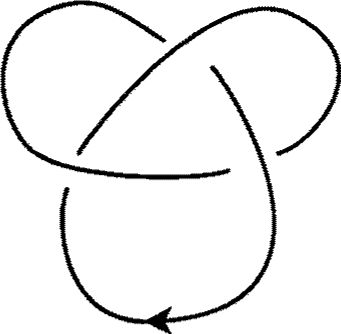
\includegraphics[width=0.25\linewidth]{figures/fig01.png}
    \caption{三维空间中的一个纽结。（原文 p.~352，Fig.~1）}
\end{figure}

% [Tutor Note: 术语] 原文 “in an intrinsically three dimensional definition” 中的
% “intrinsically three dimensional” 译为“内蕴三维的”，指不借助 $M$ 的任何二维投影或切片、
% 只用到 $M$ 本身的三维拓扑。这是本文的核心诉求：Jones 多项式应有三维的定义，
% 二维的投影算法只是计算手段。后文按层次展开这一诉求：§2 用弱耦合极限（路径积分、
% 驻相与行列式）检验理论的自洽性，§3 用正则量子化在 $\Sigma\times\mathbb{R}$ 上
% 构造物理希尔伯特空间（即共形块），§4 发展可计算性（手术公式、辫群表示），
% §5 给出对物理学的应用。

在物理方面，关于纽结多项式的疑问如下。与 Donaldson 理论（在其中与量子场论的联系并不显然）
不同，纽结多项式几乎从一开始就与二维多体物理密切相联。事实上，纽结多项式的各种构造
以令人眼花缭乱的方式把它们与二维（或 $1+1$ 维）多体物理联系起来，主要涉及可解格点模型 [7]、
Yang–Baxter 方程的解 [8]、以及共形场论的单值性 [11]。在后一种解释中，
纽结多项式与共形场论中近来成果格外丰硕的那些方面相关 [12–16]。
在统计力学方面，对纽结多项式的研究把它们与 Temperley–Lieb 代数及其推广联系起来，
也与 $1+1$ 维可解统计力学模型的其他方面相联系。对物理学家而言，
纽结多项式带来的挑战在于：为这种多样性带来秩序、找到统一的主题，
并弄清二维共形场论中究竟是什么东西是三维的。

% [Tutor Note: 物理图像] 这段话是全文的动机所在，值得逐句读。作者列出三类“二维”来源：
% (i) 可解格点模型（统计力学，Temperley–Lieb 代数是其结构代数）；(ii) Yang–Baxter 方程
% （可积性，给出 $R$ 矩阵与辫群表示）；(iii) 共形场论的单值性（Knizhnik–Zamolodchikov 方程
% 的单值性即辫群表示）。本文的贡献在于指出这三者之外还有第四条、而且是“三维”的路径：
% 三维陈–西蒙斯理论。文中“究竟是什么东西是三维的”一句，答案是：二维共形场论的共形块
% （conformal block）实为三维理论的物理希尔伯特空间（见 §3、§4）。

现在，Donaldson 理论与 Jones 理论（以及 Floer 理论与 Gromov 理论 [17]）处理的都是拓扑不变量；
而把这些理论理解为量子场论，就意味着构造出所有可观测量都是拓扑不变量的理论。
有些物理学家可能觉得这有点奇怪，所以我们先停下来解释“拓扑不变性”的物理含义。
其物理含义其实就是“广义协变性”。凡能从流形 $M$（作为拓扑空间，或许还带有光滑结构）
计算得到、而不需要选取度规的量，数学家称之为“拓扑不变量”（或“光滑不变量”）。

对物理学家而言，一个定义在流形 $M$ 上、且不先验地选取 $M$ 上度规的量子场论，
被称为是广义协变的。显然，在广义协变的量子场论中计算出的任何量都是拓扑不变量。
反过来，如果一个量子场论中所有可观测量都是拓扑不变量，
那么它自然可以看成一个广义协变的量子场论。确实，Donaldson、Floer、Jones 与 Gromov 理论
可以看成四维、三维与二维时空中的广义协变量子场论。
对物理学家来说，令人惊奇之处也许在于广义协变性是如何实现的。
广义相对论为我们提供了构造“不先验选取度规的量子场论”的原型
——我们引入一个度规，然后对所有度规积分。这个例子对我们的思维影响如此之大，
以至于我们倾向于把广义协变理论按定义理解为“度规是动力学变量”的理论。
从 Donaldson、Floer、Jones 与 Gromov 理论得到的教训恰恰是：
存在高度非平凡的量子场论，其中广义协变性以其他方式实现。
特别地，本文将描述一个可精确求解的广义协变量子场论，其中广义协变性不是通过
对所有度规积分实现的，而是因为我们从一个不含度规的规范不变拉格朗日量出发。

% [Tutor Note: 易错点] 原文“Obviously, any quantity computed in a generally covariant quantum
% field theory will be a topological invariant”中的“Obviously”藏着一个不显然的前提：
% 路径积分测度必须在流形微分同胚下不变。若测度有反常（本文 §2 会遇到的标架反常就是一个例子），
% 则配分函数只能定义在带标架的流形上，拓扑不变性被弱化为“标架化流形的微分同胚不变量”。
% 作者此处按直觉陈述，严格化要等到后面处理反常时才补上；读 §2 时应回头对照本段。
%
% [Tutor Note: 概念辨析] 这里的“广义协变”（general covariance）指“不预设背景度规”：
% 拉格朗日量本身不含度规，因而无需选取度规即可定义作用量，可观测量随之成为拓扑不变量。
% 它并不要求“度规是动力学变量、要对所有度规积分”——那只是广义相对论式的实现方式，
% 也正是作者要读者摆脱的思维定式。严格地说，广义协变性在量子层面等价于路径积分测度
% 在微分同胚下不变（见上一条批注）；经典层面本文的理论显然满足，量子层面则要等到
% 处理标架反常时才完全落实。这是全文反复强调的“另一种实现广义协变性的方式”，
% 也是把 2+1 维陈–西蒙斯理论与 1+1 维共形场论联系起来的根本原因。


% =============================================================================
%  s01-cs-action.tex —— §1 陈–西蒙斯作用量
%  原文 PDF p.3（"1. The Chern-Simons Action" 标题起）– p.6（"2. The Weak Coupling
%  Limit" 标题之前）；印刷页 353–356。编号公式 (1.1)–(1.6) 沿用原文编号，无跳号。
%  所有公式符号均据 witten1989/pages300/page-03..06.png 逐符号核对。
% =============================================================================
\section{陈–西蒙斯作用量}

\begin{keypoints}
    \item \textbf{物理图像：}陈–西蒙斯 3-形式是定向三维流形上的 3-形式，积分只需要定向、不需要度规；
          以它为拉格朗日量的规范理论因此天然广义协变，可观测量全是拓扑不变量。
    \item \textbf{数学工具：}李代数值联络 $A_i$、曲率 $F_{ij}=[D_i,D_j]$、
          陈–西蒙斯三项式 $\Tr(A\wedge\mathrm{d}A+\frac{2}{3}A\wedge A\wedge A)$，
          以及由沿闭曲线的和乐定义的威尔逊线 $W_{\mathrm{R}}(C)$。
    \item \textbf{关键结论：}作用量在绕数为 $m$ 的大规范变换下平移 $\mathrm{const}\cdot m$；
          $\exp(i\mathcal{L})$ 的单值性要求该常数为 $2\pi$ 的整数倍，从而迫使能级 $k$ 量子化。
    \item \textbf{核心断言：}链环的配分函数 (1.6) 在 $S^3$ 上复现 Jones 多项式及其两变量推广，
          在一般定向三维流形上给出其内蕴、且（如后文所示）有效可计算的推广。
\end{keypoints}

我们一直受到 [1] 的敦促，尝试用三维杨–米尔斯理论来解释 Jones 多项式。于是我们从带定向的三维流形 $M$ 出发，取紧致单群 $G$ 作为规范群。我们选取一个 $G$ 丛 $E$——它不妨取为平凡丛——并在 $E$ 上放置一个联络 $A_i^a$；该联络可以看作一个李代数值的 1-形式（其中 $a$ 遍历李代数的一组基，$i$ 是 $M$ 的切指标）。无穷小规范变换为
\begin{equation}
    A_i \to A_i - D_i\varepsilon,
    \tag{1.1}
\end{equation}
其中 $\varepsilon$ 是规范群的一个生成元，是一个李代数值的 0-形式；协变导数为 $D_i\varepsilon=\partial_i\varepsilon+[A_i,\varepsilon]$。曲率则是李代数值的 2-形式 $F_{ij}=[D_i,D_j]=\partial_iA_j-\partial_jA_i+[A_i,A_j]$。现在需要选取拉格朗日量。我们\emph{不会}选取标准的杨–米尔斯作用量\footnote{在下文中，符号“Tr”表示 $G$ 的李代数上的一个不变双线性型，即 Cartan--Killing 形式的一个倍数；其归一化我们将在随后指定。}
\begin{equation}
    \mathcal{L}_0=\int_M \sqrt{g}\,g^{ik}g^{jl}\,\Tr(F_{ij}F_{kl}),
    \tag{1.2}
\end{equation}
因为它依赖于度规 $g_{ij}$ 的选取。我们想要建立一个广义协变的理论（其中所有可观测量都将是拓扑不变量），为此我们要选取一个不需要对度规作任何选取的拉格朗日量。

% [Tutor Note: 规范变换的符号约定，此处极易出现符号错误]
% 原文取联络为反厄米（anti-Hermitian）矩阵：协变导数为
% $D_i\varepsilon=\partial_i\varepsilon+[A_i,\varepsilon]$，曲率为
% $F_{ij}=\partial_iA_j-\partial_jA_i+[A_i,A_j]$，两式中都没有显式的 $i$。
% 若换成物理文献常用的厄米生成元约定 $A_i=-igA_i^{\mathrm{h}}$，则
% $D_i=\partial_i-igA_i^{\mathrm{h}}$、$F_{ij}=\partial_iA_j^{\mathrm{h}}-\partial_jA_i^{\mathrm{h}}
% -ig[A_i^{\mathrm{h}},A_j^{\mathrm{h}}]$，且 (1.1) 中整体的负号与交换子项的符号都要重算。
% 核对 (1.1) 的自洽性：有限规范变换为 $A^g=g^{-1}Ag+g^{-1}\mathrm{d}g$，取
% $g=e^{-\varepsilon}$ 并展开到 $\varepsilon$ 的一阶，恰得 $\delta A_i=-D_i\varepsilon$，
% 与 (1.1) 一致（若取 $g=e^{+\varepsilon}$ 则得 $+D_i\varepsilon$，符号相反）。
% 本文自始至终用数学约定，§2 的平坦联络条件 $F=0$ 与 $\Tr(F\wedge F)$ 等公式均以此为准；
% 与别的文献对照前务必先统一约定。

正是在三维，存在一个合理的选择，即陈–西蒙斯 3-形式的积分：
\begin{align}
    \mathcal{L} &= \frac{k}{4\pi}\int_M \Tr\left(A\wedge \mathrm{d}A+\frac{2}{3}A\wedge A\wedge A\right) \notag\\
    &= \frac{k}{8\pi}\int_M \varepsilon^{ijk}\,\Tr\left(A_i(\partial_jA_k-\partial_kA_j)
        +\frac{2}{3}A_i[A_j,A_k]\right).
    \tag{1.3}
\end{align}

% [Tutor Note: 为什么 (1.3) 与度规无关]
% 关键有两点。(i) $A\wedge\mathrm{d}A$ 与 $A\wedge A\wedge A$ 都是微分形式，
% 被积式是一个 3-形式；3-形式在定向三维流形上的积分只需要一个定向（即一个体积形式），
% 积分本身不要求度规。对比 (1.2)：$\sqrt{g}\,g^{ik}g^{jl}$ 必须用度规来缩并 $F$ 的指标
% 并提供体积元 $\sqrt{g}\,\mathrm{d}^3x$，所以 (1.2) 依赖 $g_{ij}$，而 (1.3) 不依赖。
% (ii) 陈–西蒙斯 3-形式不是示性类：$\mathrm{d}(A\wedge\mathrm{d}A+\frac{2}{3}A^3)
% =\Tr(F\wedge F)$ 只有在把 $A$ 延拓到四维流形时才是 4-形式；在三维流形上它只是普通的
% 3-形式。对联络变分得 $\delta\mathcal{L}\propto\int_M \Tr(\delta A\wedge F)$
% （分部积分后只剩该项），故驻点条件为 $F=0$，即 §2 中式 (2.2) 的平坦联络条件。
% 这也说明 (1.3) 本身不是拓扑不变量，而是“其指数可以良定义”的次级不变量。

% [Tutor Note: $\varepsilon^{ijk}$ 约定与 (1.3) 两式系数的自洽性，极易算错]
% 本文取 $\varepsilon^{123}=+1$，并令 $\mathrm{d}x^i\wedge\mathrm{d}x^j\wedge\mathrm{d}x^k
% =\varepsilon^{ijk}\mathrm{d}^3x$。于是（对重复指标求和，无需再补 $1/2$）
% $A\wedge\mathrm{d}A=\varepsilon^{ijk}A_i\partial_jA_k\mathrm{d}^3x$、
% $A\wedge A\wedge A=\varepsilon^{ijk}A_iA_jA_k\mathrm{d}^3x$。利用 $\varepsilon^{ijk}$ 的全反对称性
% 与 Tr 的循环性可得
% $\varepsilon^{ijk}\Tr(A_iA_jA_k)=\frac{1}{2}\varepsilon^{ijk}\Tr(A_i[A_j,A_k])$。
% 于是 (1.3) 第一式的 $\frac{2}{3}A\wedge A\wedge A$ 对应第二式的 $\frac{2}{3}A_i[A_j,A_k]$
% （系数看似不变，其实来自迹恒等式的 $1/2$ 已被吸收）。第二式的 prefactor
% $\frac{k}{8\pi}$ 是第一式 $\frac{k}{4\pi}$ 的一半，这“减半”在两项中的补偿方式不同：
% 动能项中它被 $A_i(\partial_jA_k-\partial_kA_j)=2A_i\partial_jA_k$ 的因子 $2$ 抵消；
% A$^3$ 项中则正是迹恒等式的 $1/2$ 使 $\frac{k}{4\pi}\cdot\frac{2}{3}\cdot\frac{1}{2}
% =\frac{k}{8\pi}\cdot\frac{2}{3}$。可直接验算：两式的 A$^3$ 项都等于
% $\frac{k}{12\pi}\int\varepsilon^{ijk}\Tr(A_i[A_j,A_k])\mathrm{d}^3x$。核对 (1.3) 时务必把
% $\varepsilon$ 的全反对称性、Tr 的循环性与 $2/3$ 的系数三处一起算一遍。
% 文献中还有把系数写成 $k/8\pi^2$（或
% $k/4\pi^2$）的约定，那只是把 Tr 或 $A$ 另行归一化的结果，$k$ 的数值随之重标度；
% 引用具体数值时必须换算回本文 (1.3) 的 $k/4\pi$。

% [Tutor Note: 脚注 1 的“Tr”归一化]
% 脚注 1 只说明 Tr 是李代数上的不变双线性型、即 Cartan--Killing 形式 $B$ 的一个倍数，
% 具体倍数留待后文确定：原文在 (1.4) 之后说，可“唯一地确定 Tr 的归一化使 $k\in\mathbb{Z}$”。
% 对 $\mathrm{SU}(N)$，$\Tr$ 取 $N$ 维定义表示中的迹时，有 $B(X,Y)=2N\Tr_{\mathrm{fund}}(XY)$，
% 即 $\Tr_{\mathrm{fund}}=\frac{1}{2N}B$；正是这个固定的倍数使 (1.4) 中的“常数”等于 $2\pi k$
% （见下一条批注），从而 $k$ 的整数条件有确定含义。对一般单群，把 Tr 取为“长根平方为 2”
% 的归一化（Dynkin 指数为 1 的不变形式）即可得到同样的整数条件。若改用别的倍数，$k$ 会按
% 比例重标度——这正是后文把 $k$ 与共形权、$q$ 的指数联系起来的公式中，$k$ 必须用本文
% 归一化的原因。

陈–西蒙斯项在三维规范理论中有着相当长的历史。只含陈–西蒙斯项的阿贝尔规范理论曾由 Schwarz [18] 研究过，I. Singer 也在未发表的工作中研究过它。把陈–西蒙斯项加到通常作用量 (1.2) 上的三维规范理论在 [19–21] 中引入。只含陈–西蒙斯作用的非阿贝尔理论曾由 Zuckerman [22] 在经典层面研究过。阿贝尔陈–西蒙斯理论近来被 Hagen [24] 以及 Arovas 等人 [25] 与分数统计联系起来研究，并被 Polyakov [23] 与 Fröhlich [15] 与环绕数联系起来研究。我们当前讨论的新颖之处在于：我们将考虑由非阿贝尔陈–西蒙斯作用量定义的量子场论，并论证它是可精确求解的，而且对三维几何与二维共形场论有着重要意义。

陈–西蒙斯理论的第一个基本性质是首先在 [21] 中讨论过的量子化律。它之所以出现，是因为由连续映射 $M\to G$ 构成的群 $\tilde{G}$ 不是连通的。在对这类映射作同伦分类时，人们至少会遇到这样一个事实：对每个紧致单群 $G$ 都有 $\pi_3(G)\cong\mathbb{Z}$。尽管 (1.3) 在规范群中包含单位元的那个连通分支下不变，但它在绕数非零的规范变换下并非不变；这类规范变换对应于 $\pi_3(G)$ 的非零元素。在绕数为 $m$ 的规范变换下，(1.3) 的变换规律是
\begin{equation}
    \mathcal{L}\to\mathcal{L}+\mathrm{const}\cdot m.
    \tag{1.4}
\end{equation}
正如 Dirac 关于磁单极子的著名工作那样，量子场论的自洽性并不完全要求 $\mathcal{L}$ 本身单值，而只要求 $\exp(i\mathcal{L})$ 单值。为此，(1.4) 中的“常数”应当是 $2\pi$ 的整数倍，这既是必要条件也是充分条件。这就给出了对 (1.3) 中称为 $k$ 的参数的量子化条件。若 $G$ 是 $\mathrm{SU}(N)$，且“Tr”指 $N$ 维表示中的迹，则该要求是 $k$ 应为整数。一般地，对任意 $G$，我们可以唯一地确定此前尚未指定的“Tr”的归一化，使得量子化条件为 $k\in\mathbb{Z}$。

% [Tutor Note: 绕数、$\pi_3(G)$ 与 (1.4) 中的“常数”]
% 大规范变换由映射 $g:M\to G$ 给出，其绕数 $m$ 是 $g$ 在 $\pi_3(G)\cong\mathbb{Z}$ 中的类；
% $M=S^3$ 时它就是 $g$ 的映射度，一般 $M$ 上由 $H^3(M;\mathbb{Z})$ 分类。
% 若把 Tr 归一化到 $\frac{1}{24\pi^2}\int\Tr(g^{-1}\mathrm{d}g)^3\in\mathbb{Z}$（对 $\mathrm{SU}(N)$
% 的定义表示正是如此），直接计算给出
% $\Delta\mathcal{L}=\frac{k}{4\pi}\cdot\frac{1}{3}\int\Tr(g^{-1}\mathrm{d}g)^3=2\pi k\,m$，
% 即 (1.4) 中的“常数”为 $2\pi k$。于是 $\exp(i\mathcal{L})$ 单值当且仅当 $k\in\mathbb{Z}$，
% 这正是原文“necessary and sufficient”的依据；“常数”里含 $k$（而非仅含数字常数）是关键，
% 因为它把量子化条件转嫁给了耦合常数。也要注意 $m$ 的符号取决于 $M$ 与 $g$ 的定向约定，
% 但 $k\in\mathbb{Z}$ 这一条件与符号无关。

我们稍后会看到，$k$ 与仿射李代数最高权表示理论中的中心荷密切相关。表明 (1.3) 中的 $k$ 必须量子化的那套推理有一个 $1+1$ 维的类比 [26]，它导致仿射代数表示论中中心荷的量子化；这并非偶然。

\begin{figure}[htbp]
    \centering
    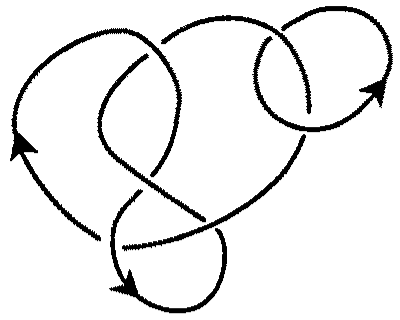
\includegraphics[width=0.28\linewidth]{figures/fig02.png}
    \caption{三维流形 $M$ 中若干相互链接但互不相交的有向纽结。这样一族纽结称为一个“链环”（link）。（原文 p.~355，Fig.~2）}
\end{figure}

在量子场论中，除拉格朗日量之外，人们还希望选取一类合适的规范不变可观测量。在当前语境下，通常的规范不变局域算子并不合适，因为它们会破坏广义协变性。然而，QCD 中为人熟知的“威尔逊线”提供了一类自然的规范不变的可观测量，它们不需要选取度规。设 $C$ 是 $M$ 中一条定向闭曲线。内蕴地看，$C$ 不过是一个圆；但圆在 $M$ 中的嵌入的拓扑分类非常复杂，正如我们在图 1 中所看到的。设 $R$ 是 $G$ 的一个不可约表示。于是把“威尔逊线”$W_{R}(C)$ 定义为联络 $A_i$ 的如下泛函：先计算 $A_i$ 绕 $C$ 的和乐，得到 $G$ 中一个在共轭意义下良定的元素，然后取该元素在表示 $R$ 中的迹。于是定义是
\begin{equation}
    W_{R}(C)=\Tr_{R}P\exp\int_C A_i\,\mathrm{d}x^i.
    \tag{1.5}
\end{equation}

这个定义的关键性质在于：不需要引入任何度规，因此广义协变性得以保持。

% [Tutor Note: 威尔逊线定义中的三个技术点]
% (i) $P$ 表示路径排序：$P\exp\int_CA_i\mathrm{d}x^i$ 是沿 $C$ 的平行移动算符（和乐），
% 由于 $A_i$ 是矩阵，路径排序不可省略；其定义依赖 $C$ 的定向，反向绕行即取逆元。
% (ii) 和乐本身是 $G$ 中的元素，只在共轭类意义下与起点处平凡化的选取无关，
% 因此必须取表示 $R$ 中的迹 $\Tr_R$，才能得到与平凡化无关的规范不变泛函——这就是
% 定义中先“算和乐”后“取迹”的原因。
% (iii) 表示标号在 (1.5) 中记作 $R$、在 (1.6) 中记作 $R_i$，二者同为一回事：(1.5) 讲单条
% 威尔逊线，(1.6) 讲链环的各分支 $C_i$；不必误以为是两个不同的量。原刊用斜体 $R$，
% 本译本统一为斜体 $R$、$R_i$（$\Sigma\times\mathbb{R}^1$ 中的 $\mathbb{R}$ 才是正体）。

现在我们可以陈述所关心的一般问题了。在带定向的三维流形 $M$ 中，取 $r$ 条定向且互不相交的纽结 $C_i$（$i=1,\dots,r$），它们的并集就是纽结理论家所称的“链环”$L$。我们给每条 $C_i$ 指定一个表示 $R_i$，并计算费曼路径积分
\begin{equation}
    \int D\mathcal{A}\,\exp(i\mathcal{L})\prod_{i=1}^{r}W_{R_i}(C_i).
    \tag{1.6}
\end{equation}
符号 $D\mathcal{A}$ 表示费曼式积分，即积遍所有规范轨道：把模去规范变换的所有联络等价类积遍。当然，(1.6) 恰好具有 QCD 中某些熟悉可观测量的形式结构，区别在于我们处在三维而非四维，并且选取了一个略显奇特的规范理论作用量。我们将把 (1.6) 称为带给定链环的 $M$ 的“配分函数”，或给定链环的（未归一化的）“期望值”；并把它记为 $Z(M;C_i,R_i)$，或简记为 $Z(M;L)$。

% [Tutor Note: 路径积分测度与“规范轨道”]
% $D\mathcal{A}$ 是形式记号，指模去规范变换后的联络空间上的积分；在无度规、无标架的
% 流形上，这一测度本身并没有严格的数学定义（这正是 §2 要先取弱耦合极限、再借
% Ray--Singer 挠率来讨论行列式的原因，见 [18] 及 §2）。此外，作用量 (1.3) 中系数含 $k$，
% 故弱耦合极限是大 $k$ 而非小 $k$：§2 式 (2.1) 的被积式是 $\exp(ik\cdot\frac{1}{4\pi}\int\Tr(\cdots))$，
% 在 $k\to\infty$ 时剧烈振荡，可用驻相法近似。读本节时不要把它与通常杨–米尔斯理论的
% $1/g^2$ 展开混为一谈。

对于 $S^3$ 中的链环情形，我们将断言：不变量 (1.6) 恰好就是 Jones 理论及其推广中出现的那些不变量。仅仅把 $S^3$ 换成一般的定向三维流形 $M$，就得到已知纽结多项式的一个非常引人入胜（而且正如我们将看到的，是有效可计算的）推广。取 $r=0$（没有纽结）时，(1.6) 给出定向三维流形 $M$ 的不变量，它们同样被证明是有效可计算的。在深入任何细节之前，让我们先指出 (1.6) 与 Jones 理论之间可能存在联系的几点初步迹象：

（1）在 (1.6) 中我们看到的是恰当的变量，即一个紧致李群 $G$、为链环 $L$ 的每个分支 $C_i$ 选取的一个表示 $R_i$，以及一个附加的变量 $k$。[在纽结理论中，人们通常作解析延拓，把 $k$ 换成复变量 $q$；但自 Jones 最初的工作起，人们就知道在 $q$ 的特殊取值处存在特殊性质。我们断言，这些性质反映了如下事实：以 (1.3) 为作用量的三维规范理论只有当 $k$ 为整数时才是良定义的。] Jones 多项式的两变量推广对应于 $G=\mathrm{SU}(N)$、且所有 $R_i$ 都取 $\mathrm{SU}(N)$ 的定义 $N$ 维表示的情形。这两个变量是 $N$ 与 $k$，它们都被解析延拓为复值。Kauffman 多项式类似地出现在 $G=\mathrm{SO}(N)$、$R$ 取 $N$ 维表示的情形。

% [Tutor Note: 方括号中的插入语]
% 原文在列举“正确的变量”时用方括号插入了一段关于 $q$ 的解析延拓的说明。它点出了
% 本文与纽结理论的关键对接方式：纯陈–西蒙斯理论只在 $k\in\mathbb{Z}$ 时良定义
% （这是 (1.4) 量子化条件的要求），而纽结多项式作为 $q$ 的（洛朗）多项式在任意 $q$
% 处有定义；把 $k$ 解析延拓为复变量（等价于把 $q$ 解析延拓）之后，整数 $k$ 处的特殊
% 性质恰好反映了“量子场论只在整数点存在”这一事实。方括号内这句话是后文 §3、§4
% 把 $Z$ 与共形场论、$q$ 联系起来的伏笔，不应略读。

（2）作为对 (1.6) 与纽结多项式之间关系之合理性的进一步检验，我们首先注意到：(1.6) 依赖于 $M$ 定向的选取，因为陈–西蒙斯形式的符号正是由定向确定的。同样，(1.6) 也依赖于 $C_i$ 的定向，因为定向进入威尔逊线的定义（在计算绕 $C_i$ 的和乐时，必须决定沿哪个方向绕 $C_i$ 积分）。然而，如果反转其中一条 $C_i$ 的定向，同时把表示 $R_i$ 换成它的复共轭 $\bar{R}_i$，则威尔逊线的定义不变，因此 (1.6) 在这一操作下不变。而如果（不改变 $R_i$）反转链环 $L$ 所有分支 $C_i$ 的定向，则 (1.6) 也不变，这是由于物理学家称之为“电荷共轭”的一种对称性。它是 $G$ 的李代数的一个对合，把所有表示换成其复共轭表示；把这一对合作用到 (1.6) 的所有积分变量上，(1.6) 保持不变，同时把所有 $R_i$ 换成其共轭表示——等价地，反转所有 $C_i$ 的定向。这些是纽结多项式的重要形式性质。

% [Tutor Note: 电荷共轭、定向与复共轭表示]
% 这里的“电荷共轭”是李代数上的一个对合（involution），它同时把每个表示 $R$ 与其
% 复共轭表示 $\bar{R}$ 互换。作用到路径积分上时，它是积分变量的一个替换，不改变积分值；
% 因此“反转所有分支的定向”与“把所有 $R_i$ 换成 $\bar{R}_i$”给出同一个不变量的两种
% 描述，而“只反转单个分支的定向”则必须同时取 $\bar{R}_i$ 才保持 (1.6) 不变——这一步
% 不是可选的约定，而是由 (1.5) 中“取表示中的迹”所强制的。这些正是纽结多项式
% 重要形式性质的场论来源：例如 Jones 多项式在取镜像（所有交叉反向）时
% $q\to q^{-1}$，以及复共轭表示取共轭等，都是这里的定向—复共轭配对在 $S^3$ 情形的
% 具体化。§2 之后把 $Z$ 与 $V_L(q)$ 的显式关系写出后，可逐条对照。
% （原文本段结束处即印刷页 356 的 "These are important formal properties of the
% knot polynomials."，紧接着是 §2 标题，由另一片段衔接。）


% =============================================================================
%  §2 弱耦合极限（The Weak Coupling Limit）
%  覆盖页段：PDF p.6（印刷 p.356，自 "2. The Weak Coupling Limit" 标题起）
%            – PDF p.11 末（印刷 p.361）
%            及 PDF p.12 顶部（印刷 p.362，"Some Examples" + 式 (2.26) + 脚注 5，
%            写到 §2.1 "Incorporation of Knots" 标题之前）
%  编号公式：(2.1)–(2.26)，与原文逐一对应，无跳号、无合并
%  说明：§2 标题确认在 PDF p.6 中部；p.6 顶部（§2 标题之前）的 §1 收尾两段
%        属 §1，不收入本片段。
% =============================================================================

\section{弱耦合极限}

\begin{keypoints}
    \item \textbf{物理图像：} 大 $k$ 时路径积分的被积函数剧烈振荡，积分由驻相点主导；陈–西蒙斯作用量的驻相点恰是平坦联络（$F=0$），弱耦合极限因此把非阿贝尔理论约化为对平坦联络的求和。
    \item \textbf{数学工具：} 高斯积分与 Faddeev--Popov 规范固定；扭曲外微分 $D$ 与 Hodge 星 $\ast$、自伴算子 $L=\ast D+D\ast$ 及其在奇阶形式上的限制 $L_-$、以及 $\zeta$ 函数正规化、$\eta$ 不变量、Atiyah--Patodi--Singer 定理与 Ray--Singer 挠率。
    \item \textbf{关键结论：} 驻相贡献为式 (2.8)；其行列式之比的绝对值是 Ray--Singer 挠率，相位由 $\eta$ 不变量给出，而 $\eta(0)$ 的度规依赖使 $k$ 被平移为 $k+c_2(G)/2$，见式 (2.17)。
    \item \textbf{标架反常：} 用引力陈–西蒙斯项 (2.20) 吸收 $\eta(0)$ 的歧义后，配分函数成为定向带标架三维流形的拓扑不变量；标架平移 $s$ 个单位时 $Z\to Z\exp(2\pi i s\,d/24)$，有限 $k$ 时 $d$ 换成中心荷 $c$。
    \item \textbf{遗留缺口：} 式 (2.8) 要求各行列式非零（等价于 $H^\ast(M,E)=0$）；否则配分函数不是式 (2.4) 的离散和，而是平坦联络模空间上的积分，鬼场还可能出现零模。
\end{keypoints}

首先，由于一个只含陈–西蒙斯作用量的非阿贝尔规范理论可能显得陌生，人们会先问：这个拉氏量是否真的导向一个合理的量子理论，是否真的能够被正规化而给出拓扑不变的结果？本节通过研究弱耦合极限来简要考察这一点，在此极限下计算相对直接。这就是大 $k$ 极限。\footnote{读者不妨记住：本节与下一节的讨论包含若干技术细节，它们是整个逻辑链条的一部分，但初读时也许并不必要。}

对大 $k$，路径积分
\begin{equation}
    Z=\int D\mathcal{A}\,\exp\left(\frac{ik}{4\pi}\int_M\operatorname{Tr}\left(A\wedge\mathrm{d}A+\frac{2}{3}A\wedge A\wedge A\right)\right)
    \tag{2.1}
\end{equation}
（暂时略去纽结）的被积函数剧烈振荡。此类积分的大 $k$ 极限由驻相点贡献之和给出。陈–西蒙斯作用量的驻相点恰是“平坦联络”，即曲率为零的规范场：
\begin{equation}
    F^a_{ij}=0.
    \tag{2.2}
\end{equation}

% [Tutor Note: 大 $k$ 驻相/鞍点近似的要点（对应 p.356 末至 p.357 的论证，式 (2.1)(2.2)(2.4)(2.8)）。
%  （i）$k$ 是写在作用量前面的整体因子，不是通常的耦合常数：陈–西蒙斯理论没有独立的耦合常数 $g$，
%  “弱耦合”正是指 $k\to\infty$。因此这里的半经典近似是**振荡积分**的驻相法（$\int e^{ikS}$，$k\to\infty$），
%  而不是 $e^{-S/g^2}$ 型积分在极小值附近的拉普拉斯法；被积因子的模长为 1，不存在“陡降”的实指数衰减。
%  （ii）临界点条件：$\delta S\propto\int_M\operatorname{Tr}(\delta A\wedge F)$（分部积分丢掉全导数项后），
%  故驻相点恰为 $F=0$，与度规无关；这是陈–西蒙斯理论“拓扑性”在弱耦合极限中的体现。
%  （iii）每个驻相点的贡献 = 被积函数在该点的值 $e^{ikI(A^{(\alpha)})}$（即式 (2.5) 的相位）
%  乘以高斯涨落（式 (2.8) 的行列式比值）；展开中无 $B$ 的线性项，正是 (2.6) 中“缺失”的那一项，
%  它为零等价于 $A^{(\alpha)}$ 是临界点。
%  （iv）与通常微扰论不同：这里没有 $1/k$ 的幂级数意义上的“圈展开”，大 $k$ 展开的每一项都保留精确相位
%  $e^{i(k+c_2/2)I}$；行列式比值只给出与 $k$ 无关的前因子。]

这类平坦联络的规范等价类对应于同态
\begin{equation}
    \phi\colon \pi_1(M)\to G,
    \tag{2.3}
\end{equation}
更确切地说，对应于这类同态在共轭之下的等价类。为简单起见，假设 $M$ 的拓扑使得同态 (2.3) 只有有限多个类，则 (2.1) 的大 $k$ 行为将是一个求和
\begin{equation}
    Z=\sum_\alpha \mu(A^{(\alpha)}),
    \tag{2.4}
\end{equation}
其中 $A^{(\alpha)}$ 是一组完备的平坦联络规范等价类，而 $\mu(A^{(\alpha)})$ 由 (2.1) 在 $A^{(\alpha)}$ 附近展开作驻相求值得到。这一约化表明：大 $k$ 下的非阿贝尔理论与阿贝尔理论密切相关。后者[18]已被证明导向 Ray--Singer 解析挠率[27]，而后者与纯拓扑的 Reidemeister 挠率密切相关。

% [Tutor Note: 平坦联络的模空间（式 (2.3)(2.4)，p.357）。平坦联络的全体模去规范变换，
%  与表示空间 $\operatorname{Hom}(\pi_1(M),G)$ 模去 $G$ 的共轭作用一一对应：沿闭路的和乐只依赖该闭路的同伦类，
%  给出同态 $\pi_1(M)\to G$；规范变换对应共轭，故规范等价类 = 共轭等价类。这个空间通常记作
%  $\mathcal{M}_{\mathrm{flat}}(M,G)$，其维数（在孤立点处为零）与 $H^1(M,\operatorname{ad}E)$ 相关。
%  注意 (2.4) 是先假设“只有有限多个类”才成立的离散和：例如 $M=S^3$（$\pi_1=1$）只有一个平凡联络，
%  而 $M=S^2\times S^1$（$\pi_1=\mathbb{Z}$）则有一整族。一般情形的修正见 p.361 “平坦联络的模空间”一段：
%  此时 (2.1) 的正确求值是模空间上的积分而非求和。]

$\mu(A^{(\alpha)})$ 可如下计算。在 (2.1) 中作变量替换 $A_i=A_i^{(\alpha)}+B_i$，其中 $B_i$ 是新的积分变量。平坦联络 $A^{(\alpha)}$ 的一个重要不变量是它的陈–西蒙斯不变量
\begin{equation}
    I(A^{(\alpha)})=\frac{1}{4\pi}\int_M\operatorname{Tr}\left(A^{(\alpha)}\wedge\mathrm{d}A^{(\alpha)}+\frac{2}{3}A^{(\alpha)}\wedge A^{(\alpha)}\wedge A^{(\alpha)}\right).
    \tag{2.5}
\end{equation}
把陈–西蒙斯作用量按 $B_i$ 的幂展开，前几项是
\begin{equation}
    \mathcal{L}=k\cdot I(A^{(\alpha)})+\frac{k}{4\pi}\int_M\operatorname{Tr}(B\wedge DB).
    \tag{2.6}
\end{equation}
这里应理解为：(2.6) 中的 $DB$ 表示 $B$ 关于背景规范场 $A^{(\alpha)}$ 的协变外微分；它不依赖于 $M$ 上的度规。一个要点是：(2.6) 中没有 $B$ 的线性项，因为 $A^{(\alpha)}$ 是作用量的临界点。

要完成 (2.6) 中的高斯积分，需要作规范固定。不作规范固定就无法进行，除非在 $M$ 上取一个度规（或以其他方式破坏问题的对称性）。取定这样一个度规之后，一个方便的规范选择是 $D_iB^i=0$（其中 $D_i$ 是由度规与背景规范场 $A^{(\alpha)}$ 构造的协变导数）。标准的 Faddeev--Popov 构造于是给出规范固定拉氏量
\begin{equation}
    \mathcal{L}_{\mathrm{gauge}}=\int_M\left(\operatorname{Tr}\phi D_iB^i+\operatorname{Tr}\bar{c}D_iD^ic\right).
    \tag{2.7}
\end{equation}
这里 $\phi$ 是强制规范条件 $D_iB^i=0$ 的拉格朗日乘子；$c$、$\bar{c}$ 是反对易的“鬼场”，引入它们是为了在规范场模去规范变换的空间上得到正确的测度。(2.6) 与 (2.7) 中可找到的 $\phi$ 和 $B$ 的二次项有自然的几何解释（阿贝尔情形见[18]）。令 $D$ 为 $M$ 上的外微分，用平坦联络 $A^{(\alpha)}$ 扭曲；令 $\ast$ 为把 $k$ 形式映为 $3-k$ 形式的 Hodge 算子。三维流形上有一个自然的自伴算子 $L=\ast D+D\ast$，它把偶数阶微分形式映为偶数阶形式，把奇数阶形式映为奇数阶形式。

记 $L_-$ 为其在奇阶形式上的限制。把 $B$ 与 $\phi$ 分别视为一形式与三形式，则 (2.6)、(2.7) 中的玻色子动能算子正是这个算子 $L_-$。鬼场的动能算子也是自然的几何算子，即拉普拉斯算子，我们称之为 $\Delta$。现在可以给出 (2.4) 中出现的驻相点贡献 $\mu(A^{(\alpha)})$ 的公式，即
\begin{equation}
    \mu(A^{(\alpha)})=\exp\left(ikI(A^{(\alpha)})\right)\cdot\frac{\det(\Delta)}{\sqrt{\det(L_-)}}.
    \tag{2.8}
\end{equation}
(2.8) 中的相位因子是 (2.1) 的被积函数在驻相点处的值；行列式（其绝对值可由 $\zeta$ 函数定义）来自对 $B$、$\phi$、$c$、$\bar{c}$ 的高斯积分。

% [Tutor Note: 算子 $L_-$ 与行列式比值 (2.8)（p.357 末–p.358，涉及 (2.6)(2.7)）。
%  （i）为什么动能算子就是 $L_-$：在三维流形上 $\ast$ 把 $k$ 形式映为 $3-k$ 形式，$D$ 把 $k$ 形式映为 $k+1$ 形式，
%  故 $\ast D$ 与 $D\ast$ 都不改变形式次数的奇偶性（$k\mapsto 2-k$ 或 $k\mapsto k$，其中越界项为零），
%  于是 $L=\ast D+D\ast$ 保持奇偶分解，可写 $L=L_+\oplus L_-$。$B$ 是一形式、$\phi$ 是三形式，二者都是**奇阶**形式，
%  故它们的二次型恰由 $L_-$ 给出——这是本段的关键，若误取 $L_+$，行列式的幂次与 $\eta$ 的符号全错。
%  （ii）行列式的幂次：$B$ 与 $\phi$ 是实的玻色场，高斯积分给出 $\det(L_-)^{-1/2}$；鬼场 $c,\bar{c}$ 是实格拉斯曼场，
%  积分给出 $\det(\Delta)^{+1}$，故比值为 $\det\Delta/\sqrt{\det L_-}$。写反（例如把分子写成 $1/\det\Delta$）会改变
%  (2.16) 中系数的幂次。
%  （iii）(2.8) 仅在 $L_-$、$\Delta$ 都无零模时成立；这正是 p.361 讨论 $H^\ast(M,E)$ 的动机。]

现在到了关键之处。为正规化路径积分，我们不得不在 $M$ 上取一个黎曼度规。因此，先验地并不明显：这样算出的 $\mu(A^{(\alpha)})$ 是否真是拓扑不变量。陈–西蒙斯理论也许带有反常，不能以广义协变的方式被正规化。幸运的是，我们可以援引[18]：那里证明了（在阿贝尔理论的语境下，但[18]的这一方面可以推广）(2.8) 中出现的行列式之比的绝对值恰是平坦联络 $A^{(\alpha)}$ 的 Ray--Singer 解析挠率，因此特别地是一个拓扑不变量。（这个行列式之比的相位更为微妙，将在后面讨论。）这是拓扑不变量确实可以从陈–西蒙斯理论得到的第一个迹象。

\subsection*{行列式的相位}

(2.8) 中行列式之比的绝对值虽是 Schwarz 很久以前讨论过的解析挠率，其相位却需要额外研究。鬼场行列式 $\det\Delta$ 是实且正的，因此真正的问题在于研究 $\det L_-$ 的相位。由于算子 $L_-$ 可解释为一个扭曲的狄拉克算子，其行列式的相位可以与奇维费米子行列式相位的已有研究[28]相联系。不过，下面我将从玻色子的观点给出相关事实的一个简短推导，在本语境中这或许更为自然。对 $B$ 与 $\phi$ 作一个无关紧要的重标度之后，所关心的积分是
\begin{equation}
    \int DB\,D\phi\,\exp\left(i\int_M\operatorname{Tr}\left(B\wedge DB+\phi\,D{*}B\right)\right).
    \tag{2.9}
\end{equation}
把变量换到算子 $L_-$ 的本征函数 $x_i$ 的正交归一基（相应本征值为 $\lambda_i$），(2.9) 变为
\begin{equation}
    \prod_i\int_{-\infty}^{\infty}\frac{\mathrm{d}x_i}{\sqrt{\pi}}\,e^{i\lambda_ix_i^2}.
    \tag{2.10}
\end{equation}
因此，需要理解的关键积分是
\begin{equation}
    I=\int_{-\infty}^{\infty}\frac{\mathrm{d}x}{\sqrt{\pi}}\,e^{i\lambda x^2},
    \tag{2.11}
\end{equation}
其中 $\lambda$ 为实数。我们把这个积分定义为绝对收敛积分
\begin{equation}
    \int_{-\infty}^{\infty}\frac{\mathrm{d}x}{\sqrt{\pi}}\,e^{i\lambda x^2}\cdot e^{-\varepsilon x^2}
    \tag{2.12}
\end{equation}
当 $\varepsilon\to0$ 时的极限。按这一定义、或按任何其他物理上合理的定义，积分 (2.11) 为
\begin{equation}
    I=\frac{1}{\sqrt{|\lambda|}}\cdot\exp\left(\frac{i\pi}{4}\operatorname{sign}\lambda\right).
    \tag{2.13}
\end{equation}
于是路径积分的相位正比于 $\sum_i\operatorname{sign}\lambda_i$；更准确地说，正比于它的正规化版本，即 Atiyah 等人[29]的“$\eta$ 不变量”：
\begin{equation}
    \eta(A^{(\alpha)})=\frac{1}{2}\lim_{s\to0}\sum_i\operatorname{sign}\lambda_i\,|\lambda_i|^{-s}.
    \tag{2.14}
\end{equation}
因此，路径积分的相位可以写成如下公式：
\begin{equation}
    \frac{1}{\sqrt{\det L_-}}=\frac{1}{\sqrt{|\det L_-|}}\cdot\exp\left(\frac{i\pi}{2}\eta(A^{(\alpha)})\right).
    \tag{2.15}
\end{equation}

% [Tutor Note: $\zeta$ 函数正规化与 $\eta$ 不变量 (2.13)(2.14)（p.359）。
%  （i）(2.11) 是条件收敛的振荡积分，逐点并不绝对收敛；(2.12) 用收敛因子 $e^{-\varepsilon x^2}$ 定义它，
%  先算绝对收敛的积分再取 $\varepsilon\to0$。算出 (2.13)：分子 $\sqrt{\pi/|\lambda|}\,e^{i(\pi/4)\operatorname{sign}\lambda}$，
%  除以 $\sqrt{\pi}$ 即得 $|\lambda|^{-1/2}e^{i(\pi/4)\operatorname{sign}\lambda}$。核对时注意 $|\lambda|$ 的绝对值与
%  $\lambda<0$ 时相位取 $-\pi/4$：若漏掉 $\operatorname{sign}\lambda$，$\eta$ 的符号会整体反号。
%  （ii）无穷多个本征值时 $\sum_i\operatorname{sign}\lambda_i$ 发散，故用 (2.14) 的正规化：以 $|\lambda_i|^{-s}$
%  作解析延拓（等价于热核/$\zeta$ 函数正规化）。**这里最容易出错的是因子 $1/2$**：Witten 把 $\eta$ 定义为
%  $\frac12\sum\operatorname{sign}\lambda_i|\lambda_i|^{-s}$（即 $\eta=\frac12(\#\{\lambda>0\}-\#\{\lambda<0\})$），
%  所以 (2.15) 的指数是 $\frac{i\pi}{2}\eta$。有些文献把 $\eta$ 定义成不带 $\frac12$ 的和，若两处混用，
%  (2.15)(2.16)(2.17) 会差 2 倍，$k$ 的平移量也会差 2 倍。
%  （iii）(2.15) 是把 (2.13) 对全部本征值取乘积并分离模长/相位的结果：$\prod|\lambda_i|^{-1/2}$ 给分母的绝对值，
%  $\exp(\frac{i\pi}{4}\sum\operatorname{sign}\lambda_i)=\exp(\frac{i\pi}{2}\eta)$ 给相位。]

利用 Atiyah--Patodi--Singer 定理可以使之更加明确；对我们的目的而言，该定理可视为一个表达 $\eta$ 对展开所绕的平坦联络 $A^{(\alpha)}$ 的依赖关系的公式。事实上，对算子 $L_-$，该公式是
\begin{equation}
    \frac{1}{2}\left(\eta(A^{(\alpha)})-\eta(0)\right)=\frac{c_2(G)}{2\pi}\cdot I(A^{(\alpha)}).
    \tag{2.16}
\end{equation}
这里 $I(A^{(\alpha)})$ 是平坦联络 $A^{(\alpha)}$ 的陈–西蒙斯不变量，定义见 (2.5)；$\eta(0)$ 是平凡规范场 $A=0$ 的 $\eta$ 不变量；$c_2(G)$ 是群 $G$ 的二次 Casimir 算子在伴随表示中的取值，其归一化使得 $c_2(SU(N))=2N$。这个因子的作用是把 (2.8) 中的 $k$ 替换为 $k+c_2(G)/2$；事实上，配分函数 (2.4) 现在可以写成
\begin{equation}
    Z=e^{i\pi\eta(0)/2}\cdot\sum_\alpha e^{i\left(k+c_2(G)/2\right)I(A^{(\alpha)})}\cdot T_\alpha
    \tag{2.17}
\end{equation}
其中 $T_\alpha$ [即 (2.8) 中行列式之比的绝对值] 是平坦联络 $A^{(\alpha)}$ 的挠率不变量。

% [Tutor Note: $k\to k+c_2(G)/2$ 的平移 (2.16)(2.17)（p.359，并见脚注 5 与 (2.26)）。
%  由 (2.15) 每个驻相点的相位是 $e^{\frac{i\pi}{2}\eta(A)}$，代入 (2.16) 得
%  $e^{\frac{i\pi}{2}\eta(A)}=e^{\frac{i\pi}{2}\eta(0)}\cdot e^{i c_2(G)I(A)}$，
%  与 $e^{ikI(A)}$ 合并即得 (2.17) 中的 $e^{i(k+c_2(G)/2)I(A)}$。也就是说：**“$k$ 的平移”来自把 $\eta$ 的
%  正规化/度规依赖部分与相位分离**，不是人为约定。$c_2(G)$ 的归一化是 $c_2(SU(N))=2N$；对 $G=SU(2)$
%  得 $c_2=4$，故 $k+c_2/2=k+2$——这正是 (2.26) 中 $k+2$ 的来源（原文脚注 5 也点明这一点），也是本文后文
%  式 (4.21) 的 $q=\exp(2\pi i/(N+k))$（对 $SU(2)$ 即 $\exp(2\pi i/(k+2))$）这类约定的来源。若改用“伴随表示 Casimir 本征值 $=N$”的常见归一化，
%  平移量会差一个因子，所有含 $k+2$ 的公式都会整体错位，核对时务必先确认 $c_2$ 的归一化。]

遗憾的是，虽然 $I(A^{(\alpha)})$ 与 $T_\alpha$ 是拓扑不变量，$\eta(0)$ 却不是；它依赖于规范固定时在 $M$ 上所选定的度规。因此，要使 (2.17) 的相位有意义，还需要进一步讨论，这放在下一小节。

在进入这场技术性讨论之前，请注意：刚才概述的计算其实有一个很有意思的副产品。(2.8) 中的 $k$ 在 (2.17) 中被替换成了 $k+c_2(G)/2$，这似乎是对下述事实作出解释的开端：在 $1+1$ 维流代数的许多公式中，量子修正的效果正是把 $k$ 替换为 $k+c_2(G)/2$。这又可能与下述事实有关：在 $1+1$ 维的各种可积模型（例如 sine-Gordon 模型）中，只要对参数值作出适当的、看似 ad hoc 的改变（类似于把 $k$ 换成 $k+c_2(G)/2$），WKB 近似就是精确的。

\subsection*{切丛的平凡化}

现在来讨论 (2.17) 中那个神秘的相位因子 $e^{i\pi\eta(0)/2}$ 应当如何理解。

首先，$\eta(0)$ 是与 (i) $M$ 上某个度规 $g$、(ii) 平凡规范场 $A=0$ 相耦合的 $L_-$ 算子的 $\eta$ 不变量。令 $d=\dim G$ 为规范群 $G$ 的维数。由于规范场是平凡的，$L_-$ 算子由 $d$ 份仅与度规耦合的纯引力 $L_-$ 算子构成。因此，作为准备，我们写出
\begin{equation}
    \eta(0)=d\cdot\eta_{\mathrm{grav}},
    \tag{2.18}
\end{equation}
其中 $\eta_{\mathrm{grav}}$ 是纯引力算子的 $\eta$ 不变量。我们那个有问题的相位因子是
\begin{equation}
    \mathcal{A}=\exp\left(\frac{id\pi}{2}\cdot\eta_{\mathrm{grav}}\right).
    \tag{2.19}
\end{equation}

现在，用陈–西蒙斯量子场论的某种特定正规化，我们得到了含有这个含糊相位因子 $\mathcal{A}$ 的公式 (2.17)。目标是找到另一种能够保持广义协变性的正规化。两种正规化之差应当是一个局部抵消项；而在本例中，由于问题相位 (2.19) 只依赖于背景度规，我们要的抵消项也只应依赖于背景度规。容易看出，具有正确性质的抵消项是引力陈–西蒙斯项的一个倍数，后者（类比于杨--米尔斯陈–西蒙斯项）定义为
\begin{equation}
    I(g)=\frac{1}{4\pi}\int_M\operatorname{Tr}\left(\omega\wedge\mathrm{d}\omega+\frac{2}{3}\omega\wedge\omega\wedge\omega\right).
    \tag{2.20}
\end{equation}
这里 $\omega$ 是 $M$ 的自旋丛上的 Levi-Civita 联络。\footnote{(2.20) 不是某个内蕴局部泛函的积分，因此它通常不会作为抵消项出现。无论“抵消项”这个词是否恰当，若希望工作在规范 $D_iA^i=0$ 中，我们都必须把 (2.20) 视为一种必须加到作用量上的修正。} $I(g)$ 的歧义与杨--米尔斯陈–西蒙斯作用量的歧义完全类似。要把 $I(g)$ 定义为一个数，需要 $M$ 的切丛的一个平凡化。虽然三维流形的切丛可以被平凡化，但没有典范的方式来做到这一点。任意两个平凡化相差一个不变地定义的整数，即相对的“扭转”数。引力陈–西蒙斯泛函具有如下性质：若 $M$ 的切丛的平凡化被扭转 $s$ 个单位，则 $I(g)$ 变换为
\begin{equation}
    I(g)\to I(g)+2\pi s.
    \tag{2.21}
\end{equation}

现在，Atiyah--Patodi--Singer 定理说，组合
\begin{equation}
    \frac{1}{2}\eta_{\mathrm{grav}}+\frac{1}{12}\cdot\frac{I(g)}{2\pi}
    \tag{2.22}
\end{equation}
是一个拓扑不变量，也就是说，它依赖于带有切丛平凡化选择的定向三维流形 $M$，而不依赖于 $M$ 的度规。\footnote{(2.22) 中关键的 $1/12$ 因子反映了如下差异：规范理论指标定理中出现的 Chern 特征 $e^x=1+x^2/2+\dots$，与引力指标定理中出现的 $\hat{A}$ 亏格 $(x/2)/\sinh(x/2)=1-x^2/24+\dots$ 之间的差异。} 因此，接下来该怎么做就很清楚了：我们把 (2.17) 中的 $\eta(0)/2$ 替换为 (2.22) 中出现的组合的 $d$ 倍[因子 $d$ 就是 (2.19) 中出现的那个]，于是 (2.17) 被替换为
\begin{equation}
    Z=\exp\left(i\pi d\left(\frac{\eta_{\mathrm{grav}}}{2}+\frac{1}{12}\cdot\frac{I(g)}{2\pi}\right)\right)\cdot\sum_\alpha e^{i\left(k+c_2(G)/2\right)I(A^{(\alpha)})}\cdot T_\alpha.
    \tag{2.23}
\end{equation}

于是，我们终于看到：陈–西蒙斯配分函数至少在大 $k$ 时，可以定义为定向的、带标架的三维流形 $M$ 的拓扑不变量（带标架的三维流形，指带有切丛平凡化的一个同伦类的流形）。

必须指定三维流形的标架，这一点看似麻烦，但并没有真正损失信息。由 (2.21) 可见，若标架平移 $s$ 个单位，配分函数变换为
\begin{equation}
    Z\to Z\cdot\exp\left(2\pi i s\cdot\frac{d}{24}\right).
    \tag{2.24}
\end{equation}
带标架的定向三维流形的拓扑不变量，连同标架改变下的变换律，与不带标架选择的定向三维流形的拓扑不变量大致同样好用。

% [Tutor Note: 标架反常与切丛平凡化 (2.19)–(2.23)，p.360–361。这是本节最易读错的逻辑链，逐环核对：
%  （i）(2.19) 的 $\mathcal{A}=\exp(\frac{id\pi}{2}\eta_{\mathrm{grav}})$ 来自 (2.18) 与 (2.17) 的 $e^{i\pi\eta(0)/2}$，其中 $\eta_{\mathrm{grav}}$
%  由度规决定，故 $\mathcal{A}$ 一般不正是一个拓扑不变量（它随度规变）。
%  （ii）引力陈–西蒙斯泛函 (2.20) 的歧义在于：它只在“选定了切丛平凡化”之后才是一个数，平凡化扭转 $s$ 个单位使
%  $I(g)\to I(g)+2\pi s$（(2.21)）。因此 $I(g)/2\pi$ 只定义到整数。
%  （iii）APS 定理把 $\frac12\eta_{\mathrm{grav}}$ 与 $\frac{1}{12}\cdot\frac{I(g)}{2\pi}$ 配成 (2.22) 这个在“定向 + 切丛平凡化同伦类”
%  意义下的拓扑不变量；系数 $1/12$ 不是约定，而是由两个指标密度（Chern 特征 $e^x=1+x^2/2+\dots$ 与
%  $\hat{A}$ 亏格 $1-x^2/24+\dots$）的相对系数 $1/2:(1/24)=12:1$ 决定的（见脚注 4）。
%  （iv）于是用 $d$ 倍 (2.22) 替换 (2.17) 中的 $\eta(0)/2$，就得到一个**只依赖定向与切丛平凡化同伦类**的配分函数 (2.23)。
%  （v）符号预警：$I(g)$ 项前的正负号取决于 $\omega$、$\varepsilon^{ijk}$ 与定向的约定。若符号取反，(2.24) 会变成
%  $Z\to Z e^{-2\pi i s d/24}$，$\S4.5$ 中与 $c/24$ 的比较也会整体反号。请以 (2.24) 的“正号”为自洽性判据反推约定。]

当然，本节的全部讨论、特别是 (2.24)，都只限于大 $k$ 的行为。在 4.5 节中我们将看到，(2.24) 到有限 $k$ 的推广是
\begin{equation}
    Z\to Z\cdot\exp\left(2\pi i s\cdot\frac{c}{24}\right),
    \tag{2.25}
\end{equation}
其中 $c$ 是规范群为 $G$、能级为 $k$ 的二维流代数的中心荷。众所周知，$c$ 的大 $k$ 极限恰为 $d$。

% [Tutor Note: 为什么配分函数只在带标架的三维流形上有定义 (2.21)(2.24)(2.25)，p.361。
%  由 (2.21)，标架平移 $s$ 个单位使 $I(g)$ 平移 $2\pi s$，代入 (2.23) 的指数（$I(g)$ 前系数为 $i\pi d\cdot\frac{1}{12}\cdot\frac{1}{2\pi}$）
%  得 $Z\to Z\exp(i\pi d s/12)=Z\exp(2\pi i s\,d/24)$，即 (2.24)。这说明 $Z$ 不是“定向三维流形”的不变量，
%  而是“定向 + 切丛平凡化同伦类”的不变量：正是通常所说的**标架反常**（framing anomaly）。原文的补救策略是
%  “不变量 + 标架变换律”这一对数据，它与不带标架选择的不变量几乎等价（因为任何三维流形都可平凡化切丛，歧义只是一个整数）。
%  (2.25) 把 $d$ 换成中心荷 $c$：有限 $k$ 时出现的 $e^{2\pi i s c/24}$ 正是二维共形场论中模变换 $T:\tau\to\tau+1$
%  的相位 $e^{2\pi i c/24}$，也正是 $\S4.5$ 手术公式里 $T$ 矩阵本征值的相位；$k\to\infty$ 时 $c\to\dim G=d$，故 (2.25) 与 (2.24) 相容。]

\subsection*{平坦联络的模空间}

上面关于大 $k$ 行为的讨论还有一个重要的缺口。公式 (2.8) 实际上只在其中出现的行列式都非零时才成立。事实上，平坦联络 $A^{(\alpha)}$ 决定一个平坦丛 $E$。当且仅当 $A^{(\alpha)}$ 使得 $M$ 上取值于 $E$ 的 de Rham 上同调为零时，(2.8) 中的行列式才非零。若 $H^1(M,E)\neq0$，则平坦联络 $A^{(\alpha)}$ 不是孤立的，而是位于一个规范不等价平坦联络的模空间 $\mathcal{S}$ 上；这时路径积分 (2.1) 的正确求值不是离散求和 (2.4)，而是 $\mathcal{S}$ 上的积分。若 $H^0(M,E)$ 非零，则上述处理中的 $\phi$、$c$、$\bar{c}$ 有零模，规范固定需要更加小心。可以相信，通过对路径积分作更细致的研究，可以在不对 $H^\ast(M,E)$ 作任何假设的情况下提取出任意平坦联络的大 $k$ 贡献。但我们不打算尝试这一点。

% [Tutor Note: 平坦联络模空间与零模条件，p.361（承接 (2.8)）。
%  （i）$L_-$ 的零模是取值于 $E$ 的调和奇阶形式，$\Delta$ 的零模是调和零阶形式（协变常值截面），
%  它们分别由 $H^1(M,E)$（及 $H^3$）与 $H^0(M,E)$ 刻画。故“行列式非零”$\Leftrightarrow H^\ast(M,E)=0$。
%  （ii）$H^1(M,E)\neq0$ 意味着平坦联络在模空间中有切向（非孤立），(2.4) 的离散和必须换成模空间 $\mathcal{S}$
%  上的积分（局部化/高斯近似在模空间上作），这正是“平坦联络模空间”一词的来历。
%  （iii）$H^0(M,E)\neq0$ 时鬼场与乘子有零模，规范固定（Faddeev--Popov 行列式）失效，需要处理零模（取 $1/\mathrm{Vol}$ 因子
%  或引入 collective coordinates）。原文用“It is plausible that ...”明确表示这一步未做，属作者自认的缺口，不是笔误。]

\subsection*{一些例子}

稍后我们将确定一些简单三维流形的配分函数，所得结果可与大 $k$ 计算相比较。对 $S^2\times S^1$，$Z=1$，与 $G$ 和 $k$ 都无关。对 $S^3$ 且 $G=SU(2)$，我们将得到公式\footnote{这个公式中出现 $k+2$，大概正是 (2.17) 中 $k+c_2(G)/2$ 的一个例证。}
\begin{equation}
    Z(S^3)=\sqrt{\frac{2}{k+2}}\,\sin\left(\frac{\pi}{k+2}\right).
    \tag{2.26}
\end{equation}
当然，在 $S^3$ 上唯一的平坦联络是平凡联络，对它 (2.8) 不成立，因为此时 $H^0(M,E)\neq0$。对 $G=SU(2)$，(2.26) 中 $Z\sim k^{-3/2}$ 的行为大概就是同调球面（其上平坦联络是孤立的）上平坦联络贡献的一般行为；知道如何从路径积分得到这一行为会很有意思。在 Donaldson 与 Floer 理论中，平凡联络具有负的形式维数，是许多微妙之处的根源。(2.26) 在大 $k$ 经典极限下的消失，似乎是对平凡联络“负维数”的一个有趣的定量反映。

% [Tutor Note: 式 (2.26) 与 $k^{-3/2}$ 的来源（p.362，§2 末尾；本式在 §4.6 才实际推导，此处为预告）。
%  取 $k\to\infty$：$\sqrt{2/(k+2)}\sim\sqrt{2/k}$，$\sin(\pi/(k+2))\sim\pi/k$，故 $Z\sim\sqrt{2}\,\pi\,k^{-3/2}$，
%  与原文所说 $Z\sim k^{-3/2}$ 一致。“负的形式维数”指在 Donaldson--Floer 理论中平凡联络的可约性使
%  ASD（反自对偶）瞬子模空间的形式维数取负值，导致其“贡献”在经典极限下趋于零；(2.26) 把这个现象定量化了。
%  注意此式不能由 (2.8) 的驻相公式直接得到，因为 $S^3$ 上 $H^0(M,E)\neq0$，正是上面所说的缺口。]

% ---------------------------------------------------------------------------
% 原文校勘（本页段 p.356–362 逐页核对后记录，供 Lead 汇总）：
%  1. p.361 第 3 段 “oreinted three manifolds”：印刷拼写错误，应为 oriented
%     （译文按 “定向的” 处理，不保留错误拼写）。
%  2. p.361 “In Sect. (4.5), we will see ...”：全文其余处均作 “Sect. 4”“Sect. 5.1”
%     “Sect. 2”，此处括号多余，疑为排版残留；译文作 “在 4.5 节中”。
%  3. p.361 脚注 4 “e^x = 1 + x^2/2 + ...” 只列出偶次项：此处 x 是 2-形式，
%     指标密度只取偶次项；按印刷原样照录（严格写为 e^x = 1 + x + x^2/2 + …）。
%  4. p.356 式 (2.1) 的积分测度写作 D𝒜，而同一式内规范场记作 A；p.360 式 (2.19)
%     又用 𝒜 记相位因子。原文记号 𝒜/A 混用，非笔误，译文分别作 $\mathcal{A}$ 与 $A$。
%  5. p.360–361 式 (2.22)(2.23) 中 I(g) 项前的正负号依赖 Levi-Civita 联络、ε^{ijk}
%     与定向的约定；已在批注中给出以 (2.24) 正号为自洽判据的核对办法。
%  6. p.359 “(2.13)... (4 sign λ)” 一类 OCR 残缺不作校勘（扫描层噪声，非印刷错误）。
% ---------------------------------------------------------------------------


% =============================================================================
%  s03-knots.tex —— §2.1 纽结的纳入
%  原文：PDF p.12（自编号小节标题 “2.1. Incorporation of Knots” 起）至 p.15 末
%  印刷页：362–365；公式编号 (2.27)–(2.33)；插图 Fig. 3a–c（原文在 p.364 顶部）
%  说明：p.12 顶部的 “Some Examples”、式 (2.26) 及其脚注 5 属 §2 结尾，见前一片段。
% =============================================================================

\subsection{纽结的纳入}
% （本节重点见 §2 开头片段）

现在我们要考虑存在纽结时的大 $k$ 行为。为简单起见，我们把讨论限制在 $S^3$ 以及
阿贝尔规范群 $G=U(1)$ 的情形。阿贝尔规范群在纽结理论的语境中相对平凡，
但它提供了一条快速而简单的途径，来确认陈–西蒙斯作用量确实给出拓扑不变量；
同时它也提供了一个简单的场合，用来说明一个对后文一切都至关重要的技术要点。

在阿贝尔理论中，规范场就是一个一形式 $A$，拉格朗日量为
\begin{equation}
    \mathcal{L}=\frac{k}{8\pi}\int_M \varepsilon^{ijk}A_i\partial_jA_k .
    \tag{2.27}
\end{equation}

% [Tutor Note: 原文笔误] 全反对称符号在原文式 (2.27) 中印成了斜体拉丁字母 $e^{ijk}$
% （可与同页式 (2.29) 的 $\varepsilon_{ijk}$、下页式 (2.30) 的 $\varepsilon_{ijk}$ 比较字形，
% 两者写法明显不同）。按上下文它只能是 Levi-Civita 符号 $\varepsilon^{ijk}$；本译本径写作
% $\varepsilon^{ijk}$，特此说明，以便读者对照原刊时不致误以为是一个张量分量 $e^{ijk}$。
%
% [Tutor Note: 归一化，易错] 式 (2.27) 的系数 $k/8\pi$ 与 §1 的式 (1.3) 同源，但从 (1.3) 约化到
% $U(1)$ 时有一个极易漏掉的因子 $2$：式 (1.3) 的二次项是
% $\varepsilon^{ijk}\mathrm{Tr}\big(A_i(\partial_jA_k-\partial_kA_j)\big)$，对 $U(1)$ 若取
% $\mathrm{Tr}=1$，则 $\varepsilon^{ijk}A_i(\partial_jA_k-\partial_kA_j)
% =2\varepsilon^{ijk}A_i\partial_jA_k$，代回 (1.3) 得到的是 $k/4\pi$；而 (2.27) 写的是 $k/8\pi$，
% 这相当于把 $U(1)$ 的不变双线性型取为 $\mathrm{Tr}=\tfrac12$（与 $SU(N)$ 基础表示
% $\mathrm{Tr}(T^aT^b)=\delta^{ab}/2$ 的约定一致）。等价地说，(2.27) 对应标准归一化
% $S=(\kappa/4\pi)\int A\wedge \mathrm{d}A$ 中的能级 $\kappa=k/2$。这不是无关紧要的
% 约定问题：下面的 (2.29) 的 $i/2k$、(2.31) 的 $2\pi i/k$、(2.32) 的 $n_a^2/k$ 全都依赖
% 这一口径，若把 $k/8\pi$ 误读成“标准能级 $k$”，所有相位会整体差一倍。

我们取若干圆 $C_a$ 与若干整数 $n_a$［它们对应于规范群 $U(1)$ 的表示］。
如本文一贯的约定，我们假设当 $a\neq b$ 时 $C_a$ 与 $C_b$ 不相交。
我们希望计算乘积
\begin{equation}
    W=\prod_{a=1}^{s}\exp\left(i n_a\int_{C_a}A\right)
    \tag{2.28}
\end{equation}
关于由 $e^{i\mathcal{L}}$ 所决定的高斯测度的期望值。正如 Polyakov 最近所讨论的
（他在论文 [23] 中提议把阿贝尔陈–西蒙斯理论用于高温超导体），结果可以写成如下形式
\begin{equation}
    \langle W\rangle=\exp\left(\frac{i}{2k}\sum_{a,b}n_an_b
    \int_{C_a}\mathrm{d}x^i\int_{C_b}\mathrm{d}y^j\,
    \varepsilon_{ijk}\frac{(x-y)^k}{|x-y|^3}\right).
    \tag{2.29}
\end{equation}

% [Tutor Note: 高斯积分与“指数化”] (2.29) 是纯粹的高斯积分的结果。(2.27) 是二次型，
% 而 (2.28) 中的威尔逊线只是外源：把 $A$ 的二次型配成完全平方后积掉 $A$，就得到
% $\langle W\rangle=\exp\Big[\tfrac12\sum_{a,b}n_an_b\oint_{C_a}\!\mathrm{d}x^i
% \oint_{C_b}\!\mathrm{d}y^j\langle A_i(x)A_j(y)\rangle\Big]$，其中的核
% $\varepsilon_{ijk}(x-y)^k/|x-y|^3$ 就是立体角（环绕数）核，其强度按 $1/k$ 指数化。
% 关键点有三：(i) 既然积分严格是二次的，“指数化”对任意多个威尔逊线的乘积
% 都精确成立，没有高阶修正；(ii) 相位中只有依赖环绕数的部分与度规无关，其余部分
% 在“把 $S^3$ 的一块区域认同为欧氏空间”的过程中被丢掉，这正是拓扑不变性的来源；
% (iii) 系数 $i/2k$ 与 (2.30) 的 $1/4\pi$ 相乘给出 $i/2k\cdot 4\pi=2\pi i/k$，
% 恰好是 (2.31) 的系数——核对相位时请以此链条自检，任何一处丢了 $2$ 或 $4\pi$
% 都会破坏 (2.29)→(2.31)→(2.32) 的一致性。另需注意：(2.31) 的求和 $\sum_{a,b}$
% 仍然包含 $a=b$ 项，正文说“若能忽略 $a=b$ 的项”只是暂时无视它定义不良，
% 并非把它从求和中删去。

这里把 $S^3$ 中包含这些纽结的一个区域 $U$ 与三维欧氏空间的一个区域等同起来，
$x^i$、$y^j$ 则是 $U$ 中沿纽结取值的欧氏坐标。当 $a\neq b$ 时，式 (2.29) 中的积分
本质上就是高斯环绕数，它可以写成
\begin{equation}
    \Phi(C_a,C_b)=\frac{1}{4\pi}\int_{C_a}\mathrm{d}x^i\int_{C_b}\mathrm{d}y^j\,
    \varepsilon_{ijk}\frac{(x-y)^k}{|x-y|^3}.
    \tag{2.30}
\end{equation}

% [Tutor Note: 高斯环绕积分] (2.30) 即经典的高斯环绕积分（Gauss linking integral）：
% 系数 $1/4\pi$ 是立体角归一化，它使 $\Phi(C_a,C_b)$ 成为 $C_a$ 与 $C_b$ 的环绕数
% $\mathrm{Lk}(C_a,C_b)$，当两条曲线不相交时取整数值，且与度规、与任何投影方式无关——
% 这是“陈–西蒙斯理论确实给出拓扑不变量”的第一个直接证据。几何上它等于 $C_a$ 与
% “以 $C_b$ 为边界的任一曲面”的相交数。注意被积核在对角线 $x=y$ 上按 $1/|x-y|^2$
% 奇异；$a\neq b$ 且两条曲线不相交时积分路径完全避开奇点，发散不出现，
% 此时“整数值”才是良定义的。一旦 $a=b$，同一表达式就必须先正规化（见下）。

只要 $C_a$ 与 $C_b$ 不相交，$\Phi(C_a,C_b)$ 就是一个定义良好的整数；
事实上，它是纽结理论中最经典的不变量。因此，如果能够忽略 $a=b$ 的项，
我们就会得到
\begin{equation}
    \langle W\rangle=\exp\left(\frac{2\pi i}{k}\sum_{a,b}
    n_an_b\,\Phi(C_a,C_b)\right).
    \tag{2.31}
\end{equation}

高斯环绕数的出现说明了这样一个事实：陈–西蒙斯理论确实如我们所期望的那样
给出拓扑不变量。但我们必须操心 $a=b$ 的项。这个积分在 $x=y$ 附近定义不良；
我们应当如何解释它呢？

在纽结理论中众所周知，没有任何自然且拓扑不变的办法来正规化一个纽结的自环绕数。
Polyakov 在 [23] 中使用了一种并非广义协变的正规化，由此得到的答案在几何上很有意思，
却不是拓扑不变量。对本文这种以广义协变性为首要目标的处理来说，我们需要另一条途径。
虽然并不存在 Polyakov 正规化的完全不变的替代品——也就是说，无法从带有 $a=b$ 的
式 (2.29) 或 (2.30) 中的积分得到自然的拓扑不变量——我们却不能简单地把自环绕项
及其非阿贝尔推广（它们在图 3a 中示意）丢掉，因为这些项实际上并不自然地为零。
\begin{figure}[htbp]
    \centering
    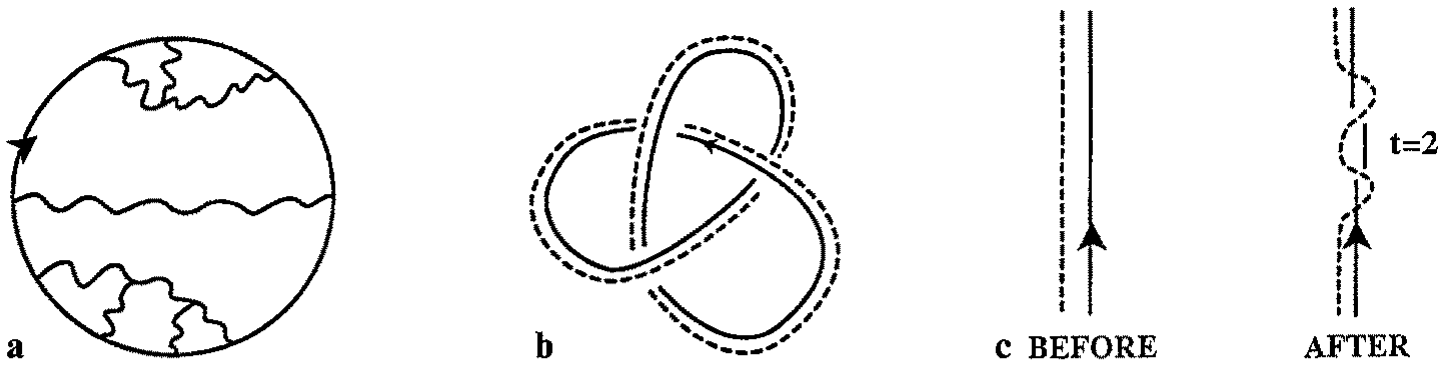
\includegraphics[width=1.00\linewidth]{figures/fig03.png}
    \caption{在非阿贝尔理论中，自环绕积分是无穷多项费曼图的首项（见 a）：规范场由同一个纽结发出并吸收，这些图都带来同样的困难。若假定每个纽结都是“带标架的”（framed，见 b），则可得到一个拓扑不变、但并非唯一确定的规则化。在 c 中，做一个二重扭转使标架移动 2 个单位。（原文 p.~364，Fig.~3）}
\end{figure}
没有理由认为丢掉这些项还能保住广义协变性。在阿贝尔理论中，一般三维流形 $M$ 上，
从拓扑上看自环绕数可以是一个非零的分数，只模 $1$ 才有定义。在那种情形下，
把自环绕数取为零不可能是正确的，因为它显然并不是零。［从拓扑上说，在这种情形下
自环绕数只能模一个整数才有定义，而这样的精度绝对不足以用来计算 (2.31)。］
在非阿贝尔理论中，我们后面会得到一些结果，它们相当于给自环绕积分的非阿贝尔推广
指定确定的、非零的值；因此，试图把这些项丢掉并不是正确的方向。

% [Tutor Note: 为什么必须给纽结指定标架] $a=b$ 项（自环绕项）无法回避，原因值得想清楚：
% (i) 式 (2.30) 的被积核在对角线 $x=y$ 上奇异，而“把 $C$ 与它自己比较”本身没有意义；
% 要定义自环绕，必须把 $C$ 与它沿法向的一个微小位移 $C'$ 作比较，而“沿哪个法向位移”
% 正是额外数据；(ii) 一般三维流形上，自环绕数只能定义到模 $1$（即取值于 $\mathbb{Q}/\mathbb{Z}$），
% 因为式 (2.31) 的相位是 $\exp(2\pi i n_a^2\Phi/k)$，当 $\Phi\to\Phi+1$ 时相位改变
% $\exp(2\pi i n_a^2/k)$，一般不是 $1$——所以“模 $1$ 的精度”确实不够用，正文的方括号
% 说的就是这个意思；(iii) 在 $S^3$ 上每个纽结都有典范（“零”）标架，由要求自环绕数为零
% 确定，但典范标架不被手术等自然操作保持，因此不能只靠它。物理上，标架就是
% 点分裂正规化所需的“第二根曲线”，它使自环绕积分的含义确定下来。原文用词
% framing（标架）与 §1 中三维流形的标架化（切丛平凡化）是同一个词，脚注 6 对此作了说明。

从拓扑上看，要理解一个纽结 $C$ 的自环绕，需要什么数据是清楚的。必须给 $C$
指定一个“标架”（framing），即沿 $C$ 的一个法向量场。其想法是：沿着这个向量场的方向
把 $C$ 稍微移动一下，就得到一个新纽结 $C'$，于是可以计算 $C$ 与 $C'$ 的环绕数。
这个环绕数就可以定义为带标架的纽结 $C$ 的自环绕数。也可以把标架想象成
把纽结加粗成一条以 $C$ 与 $C'$ 为边界的小带子；图 3b 就是这样画的。
显然，这样定义的自环绕数并不依赖于把 $C$ 移到 $C'$ 所用的具体向量场，
而只依赖于这个向量场的拓扑类；事实上，所谓“标架”，我们指的就只是它的拓扑类。
虽然选定标架给出了纽结 $C$ 自环绕数的一个定义，但同样清楚的是：只要给 $C$
挑一个方便的标架，就能得到其自环绕数的任意想要的值；如图 3c 所示，
把 $C$ 的标架扭 $t$ 圈（$t$-fold twist），会使它的自环绕数改变 $t$。\footnote{%
上述讨论应当已经表明：必须给纽结指定标架，这与上一节中必须给三维流形指定标架
是类似的需求。这有望说明，在两种情形下使用同一个词“标架”是合理的。}

从物理上说，标架的作用在于：它使物理学家所谓的点分裂正规化
（point-splitting regularization）成为可能。其定义如下：当需要计算式 (2.29) 中的
自环绕积分时，让 $x$ 沿着 $C$ 跑、$y$ 沿着 $C'$ 跑。这样得到的积分是定义良好的，
当然它依赖于标架。在本文中，我们将不加证明地假定：标架提供了足够的信息，
使得自环绕积分的一切非阿贝尔推广都能在不作进一步任意选择的情况下
得到自洽的点分裂正规化。这个问题也许可以与另一个问题相提并论：非阿贝尔
陈–西蒙斯作用量本身是否定义了一个合理的量子理论（甚至在不引入威尔逊线
作为可观测量时）。这两个问题在本文中都不会被处理。

% [Tutor Note: “a=b”短距修正与正规化] 所谓 $a=b$ 项就是自环绕积分，其短距行为是
% 全部麻烦的来源：$x$ 与 $y$ 沿同一条曲线走到一起（$|\tau-\tau'|\to0$）时，
% 被积核按 $1/|x-y|^2$ 奇异，式 (2.30) 的写法在此没有意义。正文的做法是点分裂：
% 让 $x$ 走在 $C$ 上、$y$ 走在位移后的 $C'$ 上，两条曲线保持一个小的、由标架决定的
% 间距，于是奇异性被一个有限的、但依赖标架的答案取代。也就是说，“正规化”在这里
% 不是技术细节，而是赋予了自环绕数一个确定（却非自然唯一）的值；不同的标架给出
% 相差整数（从而相差一个已知相位）的结果，这正由 (2.32) 描述。非阿贝尔情形更复杂：
% 自环绕积分的推广是无穷级费曼图之和（见图 3a：规范场从同一个纽结上发出并吸收），
% 每一阶都有同样的短距问题，而“标架足以同时正规化所有阶”只是本文的一个假定，
% 作者明确说未加证明。

当然，如果总能给纽结挑一个典范标架，那么我们只要挑这个标架就可以把问题掩盖起来。
在 $S^3$ 上，每个纽结都有一个典范标架；它由要求自环绕数为零而确定。
（这使阿贝尔环绕积分为零，但不能使其非阿贝尔推广为零。）在一般三维流形上
这做不到，因为自环绕数可能定义不良，或者可能与某个整数相差一个确定的分数
（从而无论怎样选标架都不会为零）。即使典范标架存在，把自己限制在只用它
也不方便，因为自然的操作（例如我们在 §4 中研究的手术）可能并不保持它。

因此，一般来说，我们放弃寻找自然的选择，而干脆随便挑一个标架然后继续。
如果“物理的”结果无法控制地依赖于纽结的标架，那将相当令人不快。挽救局面的是：
虽然一般说来我们无法对标架作自然选择，我们却可以陈述一条一般规则，说明
威尔逊线的期望值在标架改变时如何变化。首先让我们注意：虽然在三维流形中，
一个纽结的容许标架集合一般没有典范的零点，但只要比较两个标架，
它们总是相差一个确定的整数，即绕纽结一周时的相对扭转（图 3c）。
（也就是说，一般并没有自然的方式去数图 3b 中带子被扭了多少圈，
但存在一个自然的局部操作，可以给这条带子额外加上 $t$ 个扭转。）
在阿贝尔理论中，由 (2.29) 与 (2.30) 可以清楚地看出配分函数在标架改变时如何变换。
若把链环 $C_a$ 的标架平移 $t$ 个单位，它的自环绕数就增加 $t$，
而配分函数则移动一个相位
\begin{equation}
    \langle W\rangle\to\exp\left(2\pi i t\cdot (n_a^2/k)\right)\cdot\langle W\rangle .
    \tag{2.32}
\end{equation}

该结果的非阿贝尔类比将在 §5.1 中导出；非阿贝尔情形的变换律是
\begin{equation}
    \langle W\rangle\to\exp\left(2\pi i t\cdot h\right)\langle W\rangle ,
    \tag{2.33}
\end{equation}
其中 $h$ 是某个 $1+1$ 维流代数中初级场的共形权。这个结果虽然看起来相当技术性，
却是使陈–西蒙斯理论能够成立的关键要素。它的意思是：虽然我们必须为每一个链环
挑选标架（因为自环绕积分没有自然的定义），但信息并没有丢失，因为我们有一条
确定的定律，说明配分函数在标架改变时如何变换。

% [Tutor Note: 变换律里的因子 2，请核对] 把阿贝尔的 (2.32) 与非阿贝尔的 (2.33) 并排看：
% 两者同是“标架平移 $t$ 单位”的效应，非阿贝尔情形是 $\exp(2\pi i t\,h)$，阿贝尔情形是
% $\exp(2\pi i t\,(n_a^2/k))$。正文随后又说，阿贝尔情形的分数量子统计参数是
% $\delta=n_a^2/2k$，而非阿贝尔情形是 $\delta=h$；但“$2\pi$ 旋转的相位是 $e^{2\pi i\delta}$”
% 与 (2.32) 对照，由 (2.32) 读出的是 $\delta=n_a^2/k$，恰好是正文所写的 $n_a^2/2k$ 的两倍。
% 换句话说，若以 (2.32) 为准，则 $\delta$ 应为 $n_a^2/k$；若以正文的 $\delta=n_a^2/2k$ 为准，
% 则 (2.32) 的分母应写成 $2k$。结合上一条关于 $U(1)$ 归一化的批注：标准归一化
% $(\kappa/4\pi)\int A\wedge \mathrm{d}A$ 下自由玻色子的共形权是 $h=n^2/(2\kappa)$，
% 而 (2.27) 对应 $\kappa=k/2$，代进去正好得到 $n^2/k$。所以此处差因子 $2$ 很可能源于
% 能级口径的混用。引用这一结果时请以 (2.32) 的显式相位为准，并核对所引文献的
% 陈–西蒙斯能级约定；这是本页最容易出错的一处。

事实上可以证明 [13]：有理共形场论的结构要求存在非平凡的单值性。
在我们将要建立起来的 $2+1$ 维陈–西蒙斯理论与 $1+1$ 维有理共形场论之间的关系中，
“必须为所有纽结指定标架”正是 $1+1$ 维中出现的单值性的 $2+1$ 维类比。
［这一点在 (2.33) 的推导中会变得清楚。］若不是“必须给纽结指定标架才能把
威尔逊线定义为量子可观测量”这一看似恼人的事实，人们最终就会证明
Jones 纽结不变量是平凡的。

另一种描述可以使纽结标架的物理解释更加透明。一条威尔逊线可以看作
一个带电粒子的时空轨迹。在 $2+1$ 维中，粒子可以具有分数量子统计，
即量子波函数在旋转 $2\pi$ 后改变一个相位 $e^{2\pi i\delta}$。
（关于这些问题的讨论见 [30]。）如果想计算一个涉及分数量子统计粒子传播的
量子振幅，仅指定粒子的轨道是不够的；还必须数出粒子在其运动过程中
经历了多少次 $2\pi$ 旋转。式 (2.32) 与 (2.33) 意味着：在陈–西蒙斯理论中，
由威尔逊线所代表的粒子具有分数量子统计，阿贝尔情形下 $\delta=n_a^2/2k$，
非阿贝尔情形下 $\delta=h$。这种分数量子统计正是 Polyakov 在 [23] 中所宣称的现象；
所以在实质上我们同意他的论断，只是我们更愿意在一个广义协变的正规化框架中
展示这一现象——在其中，它表现为威尔逊线在标架改变下的行为。

% [Tutor Note: U(1) 与一般 G 的差别] 这一节之所以先做阿贝尔情形，是因为两者的难度
% 完全不在一个层次上：(i) $U(1)$ 情形下路径积分是纯高斯型，威尔逊线只是外源，
% 于是 (2.29) 精确、封闭、无需微扰展开；(ii) 自环绕项在 $U(1)$ 情形下只是“一个”
% 需要正规化的积分，而在非阿贝尔情形下它是无穷级费曼图（图 3a）之和，每一阶都要
% 单独正规化；(iii) 标架在阿贝尔情形给出一个显式的相位 (2.32)，可以直接验证；
% 非阿贝尔情形的变换律 (2.33) 要到 §5 才能从共形场论（共形权 $h$）推出；
% (iv) 阿贝尔情形的“分数量子统计”参数是 $\delta=n_a^2/2k$（与 $U(1)_k$ 的电荷–自旋关系
% 对应），非阿贝尔情形则是 $\delta=h$，其中 $h$ 依赖所插入的初级场——这正是
% Jones 多项式能编码表示论信息的原因。不要把 (2.32) 的相位当成一般的非阿贝尔公式，
% 它只是“每个威尔逊线按 $n_a^2$ 二次地”这一阿贝尔特有性质的产物。

在这一节中，我们获得了一些重要的证据，说明陈–西蒙斯理论可以被正规化，
从而给出三维流形与纽结的不变量。我们还获得了一个重要的洞见：要做到这一点，
必须选取切丛平凡化的一个同伦类，并给所有纽结指定一个“标架”。
要真正解出这个理论需要非常不同的方法，我们将在下一节转向它们。

% ---------------------------------------------------------------------------
%  原文校勘（本页段 p.362–365 逐页核对后记录，供 Lead 汇总）
%  1. p.362 式 (2.27)：全反对称符号印作斜体拉丁字母 $e^{ijk}$（与同页 (2.29)、
%     p.363 (2.30) 的 $\varepsilon_{ijk}$ 字形明显不同）。按上下文应为
%     $\varepsilon^{ijk}$。译文径改，见式 (2.27) 后第一条批注。
%  2. p.362 式 (2.27) 的 $k/8\pi$：这不是排印错误，而是 $U(1)$ 迹归一化的约定
%     （从 (1.3) 约化时 $\mathrm{Tr}$ 取 $1/2$，等价于标准能级 $\kappa=k/2$）；
%     译文照排，并在批注中给出核对链条。
%  3. p.365 “$\delta=n_a^2/2k$”与式 (2.32) 的显式相位 $\exp(2\pi i t\,n_a^2/k)$
%     相差一个因子 2（若把 $\delta$ 定义为 $2\pi$ 旋转的相位 $e^{2\pi i\delta}$，
%     则 (2.32) 给出的是 $n_a^2/k$）。疑为能级口径混用所致；译文照原文保留，
%     并在 (2.32) 后批注提示，未擅改。
%  4. p.364 图注：扫描图作 “Fig. 3a--c”，OCR 文字层误识为 “Fig. 3a-e”；
%     正文只用到 3a、3b、3c，按扫描图为准。
%  5. OCR 噪音（非印刷错误，不保留）：p.363 “As tong as” 应为 “As long as”；
%     p.365 “otherweise” 应为 “otherwise”。
%  6. p.362 式 (2.27) 的积分原文只写 $\int_M$ 而未写 $\mathrm{d}^3x$（下文记作
%     体积形式），照原文保留，未补测度。
% ---------------------------------------------------------------------------


% =============================================================================
%  s04-canonical.tex —— 第 3 节「正则量子化」
%  原文 PDF p.16–20（印刷页 366–370）：
%    3. Canonical Quantization（p.366–368）
%    3.1 The Holomorphic Viewpoint（p.368–369）
%    3.2 A Flat Vector Bundle on Moduli Space（p.369–370，本片段止于 p.370 页末；
%        该处句子跨页未完，续文在 p.371，由后续片段承接）
%  公式编号：原文 (3.1)–(3.3) 全部在本片段内，逐一对应、不跳号。
%  图：原文 p.366 顶部（位于 §3 标题之前）为 Fig. 4a–b 及其图注，本片段只标记一次。
% =============================================================================

\section{正则量子化}

\begin{keypoints}
    \item \textbf{物理图像：}把三维流形 $M$ 沿黎曼面 $\Sigma$ 切开，在 $\Sigma\times\mathbb{R}^1$ 上做正则量子化；
          所得物理希尔伯特空间 $\mathcal{H}_\Sigma$ 是有限维的，其维数由“相空间体积”控制。
    \item \textbf{数学工具：}由陈–西蒙斯作用量读出辛形式与泊松括号；高斯定律约束把相空间辛商化为
          $\Sigma$ 上平坦联络的模空间 $\mathcal{M}$；再用 Kähler 极化把量子化化为“全纯截面空间”。
    \item \textbf{关键结论：}选取复结构 $J$ 后，$\mathcal{M}$ 就是稳定全纯 $G_{\mathbb{C}}$ 丛的 Kähler 模空间，
          而 $\mathcal{H}_\Sigma$ 是行列式线丛的 $k$ 次幂 $L^{\otimes k}$ 的全纯截面空间。
    \item \textbf{结构意义：}随 $J$ 变化的 $\mathcal{H}_\Sigma^{(J)}$ 构成复结构模空间上的（射影）平坦向量丛；
          “与 $J$ 无关”等价于该丛具有典范平坦联络——这是共形块、模函子与 2+1 维理论相互沟通的接口。
\end{keypoints}

% 原文 PDF p.16（印刷 p.366）顶部为 Fig. 4a–b 及图注（“Cutting a three manifold $M$ on an
% intermediate Riemann surface $\Sigma$ …”），位置在本节标题之前；图与图注由 Lead 统一处理，
% 此处仅在原文对应位置标记一次：
\begin{figure}[htbp]
    \centering
    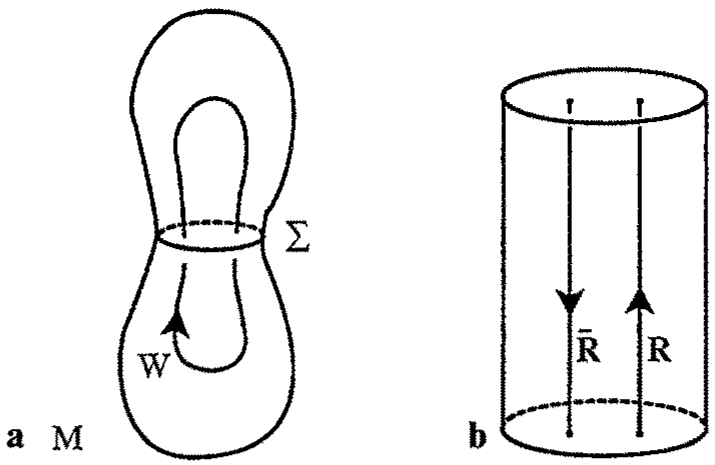
\includegraphics[width=0.49\linewidth]{figures/fig04.png}
    \caption{如 a 所示，沿中间的黎曼面 $\Sigma$ 把三维流形 $M$ 切开。$M$ 上的威尔逊线 $W$ 可能穿过 $\Sigma$；此时 $\Sigma$ 带有若干附有表示的“标记点”。局部地，在 $\Sigma$ 附近 $M$ 形如 $\Sigma\times\mathbb{R}^1$，如 b 所示。（原文 p.~366，Fig.~4）}
\end{figure}

求解任意三维流形 $M$ 上带陈–西蒙斯作用量的杨–米尔斯理论，基本策略是建立一套机制：
把 $M$ 切成若干块，在每一块上求解，再把各部分粘合回去。为此，我们先考虑一个三维流形
$M$（可能带有威尔逊线），如图 4a 所示。我们沿一个黎曼面 $\Sigma$ 把 $M$“切开”。
在切口附近，$M$ 看起来像 $\Sigma\times\mathbb{R}^1$；因此，要学会理解任意三维流形上的这个理论，
第一步就是先在 $\Sigma\times\mathbb{R}^1$ 上求解它。

形如 $\Sigma\times\mathbb{R}^1$ 的三维流形这一特殊情形，可以用正则量子化来处理。
在 $\Sigma\times\mathbb{R}^1$ 上作正则量子化，将产生一个希尔伯特空间 $\mathcal{H}_\Sigma$，
即“在 $\Sigma$ 上量子化的陈–西蒙斯理论的物理希尔伯特空间”。%
\footnote{在物理学中，习惯上把这样得到的向量空间称为“希尔伯特空间”，本译本沿用这一术语。
事实上，从路径积分最自然地得出、并且我们实际会用到的论断只是：$\mathcal{H}_\Sigma$ 是典范联系于
$\Sigma$ 的向量空间，并且当 $\Sigma$ 的定向反转时，它与自己的对偶空间互换。然而在哈密顿观点下，
希尔伯特空间结构是自然的；而对这里的具体问题而言，$\mathcal{H}_\Sigma$ 上的内积在共形场论一些
更精细的方面很重要：用 Friedan 与 Shenker [31] 的话说，这样的内积给出了“平坦向量丛上的一个度规”。
按照 Segal [16]，$\mathcal{H}_\Sigma$ 事实上具有典范的射影希尔伯特空间结构。}
后面会看到，这些空间都是有限维的，而且它们在共形场论中早已扮演过引人注目的角色。
在有理共形场论中，人们会遇到 Belavin、Polyakov 与 Zamolodchikov 的“共形块”。
Segal 用“模函子”（modular functor）来表述这些对象：模函子典范地把一个希尔伯特空间联系到一个
黎曼面上；他还以代数几何的语言描述了一类特殊的模函子，这类模函子出现在紧群 $G$ 在能级 $k$ 处的
流代数中 [16]。本文的关键观察其实就是：恰恰是这些函子，可以通过对三维量子场论作量子化而得到；
而共形场论的这一三维侧面，正是理解 Jones 多项式的钥匙。

实际上，必须研究的一般情形是：$M$ 上可能存在的威尔逊线被 $\Sigma$“切开”，如图所示。
此时 $\Sigma$ 上出现有限多个标记点 $P_1,\dots,P_k$，每个标记点 $P_i$ 上附有 $G$ 的一个表示 $R_i$
（因为每条威尔逊线都对应一个表示）。对于这样的数据——一个带标记点的定向拓扑曲面，
以及每个标记点处 $G$ 的一个表示——我们希望联系一个向量空间。这也正是共形场论中出现的一般情形：
标记点就是插入了具有非真空量子数的算符的那些点。如果把 $\Sigma$ 的定向反转
（同时把标记点所对应的表示 $R_i$ 换成其复共轭表示），则向量空间 $\mathcal{H}_\Sigma$ 必须换成它的对偶空间。

% [Tutor Note: 术语] “marked points”译“标记点”，即共形场论中插入初级场（primary field）的点；
% 本段把“每条威尔逊线对应一个表示”与“标记点处插入非真空量子数的算符”对应起来，这是全文
% “三维理论 ↔ 二维共形场论”字典的第一条：三维中的威尔逊线在二维截面 $\Sigma$ 上留下带表示的标记点。
% 后文 §3.3 与 §4 会把 $R_i$ 具体化为流代数表示，并用它们构造带穿孔的共形块。

\textbf{正则形式（The Canonical Formalism）。}乍看之下，式 (1.3) 也许像是一个典型的、无法处理的非线性量子场论；
但事实远非如此。在 $\Sigma\times\mathbb{R}^1$ 上工作时，选取规范 $A_0=0$ 是非常自然的
（这里 $A_0$ 是联络沿 $\mathbb{R}^1$ 方向的分量）。在这个规范下，我们立刻看到拉格朗日量变成二次型。
它化为

\begin{equation}
    \mathcal{L} = \frac{k}{8\pi}\int \mathrm{d}t \int_{\Sigma} \varepsilon^{ij}\,\Tr A_i\,\frac{\mathrm{d}}{\mathrm{d}t}A_j .
    \tag{3.1}
\end{equation}

% [Tutor Note: 易错点——“立刻看到”跳过了什么] 取 $A_0=0$ 后，(1.3) 中含 $A_0$ 的项全部消失；
% 而三阶项 $\varepsilon^{ijk}\Tr A_i[A_j,A_k]$ 要求 $i,j,k$ 三个指标互不相同，在 $\Sigma\times\mathbb{R}^1$
% 上除时间指标外只剩两个空间指标，故三阶项为零——这正是“becomes quadratic”的全部内容。
% 换言之，(1.3) 的立方相互作用在 $A_0=0$ 规范中被冻结，其非线性全部转移到了 (3.3) 的高斯定律约束里。
% 另注意 (3.1) 已是一阶于时间导数（这正是脚注 8 的要点）：$A_i$ 本身就是正则坐标，无需再引入动量；
% 而 $A_0=0$ 并未完全固定规范，剩余的是与时间无关的规范变换，其生成元正是高斯定律约束。

眼下我们先忽略 $\Sigma\times\mathbb{R}^1$ 上可能存在的威尔逊线所引起的额外复杂性。
由式 (3.1) 可以推出泊松括号，\footnote{这是一个典型的问题：在其中“引入正则动量”并不恰当。
引入这类变量的目的，是把一个给定的拉格朗日量重新表述为一阶于时间导数的形式；而式 (3.1) 已经
是一阶于时间导数的了。式 (3.1) 中的变量本身就是正则共轭的，正如接下来的方程所示。}

\begin{equation}
    \{A_i^a(x), A_j^b(y)\} = \frac{4\pi}{k}\cdot\varepsilon_{ij}\delta^{ab}\,\delta^2(x-y).
    \tag{3.2}
\end{equation}

% [Tutor Note: 归一化陷阱] 由 (3.1) 读出的正则 1-形式为 $\theta=\frac{k}{8\pi}\int_\Sigma
% \varepsilon^{ij}\Tr A_i\,\delta A_j$，故辛形式为 $\omega=\delta\theta=\frac{k}{8\pi}\int_\Sigma
% \varepsilon^{ij}\Tr\delta A_i\wedge\delta A_j$；(3.2) 正是它的逆。核对系数时有三处极易出错：
% 其一，(1.3) 与 (3.1) 中的 $k/8\pi$ 与 Witten 对 $\Tr$ 的归一化是配套的（归一化由 (1.3) 下方
% “$k$ 应取整数”的量子化条件固定）；若改用物理文献常见的 $\Tr(T^aT^b)=\frac12\delta^{ab}$，
% 则 (3.1) 的系数应相应改为 $k/4\pi$，否则由同一 $\theta$ 算出的括号会与 (3.2) 相差因子 2。
% 其二，(3.1) 用 $\varepsilon^{ij}$、(3.2) 用 $\varepsilon_{ij}$，二者的符号取决于 $\Sigma$ 的定向约定，
% 定向反转会使 (3.2) 整体变号。其三，这是等时（$x^0=y^0$）括号，$\delta^2$ 是 $\Sigma$ 上的二维
% $\delta$ 函数。
% 做具体计算前，建议先用 $G=U(1)$（阿贝尔情形，(3.1) 与 (3.2) 不变）验算一遍，
% 再回到非阿贝尔情形，这样最容易发现 $\Tr$ 与 $\varepsilon$ 约定上的不一致。

在急于量子化这些对易关系之前，我们应当记住：系统还受一个“高斯定律”约束，
即 $\delta\mathcal{L}/\delta A_0=0$；或者（忽略威尔逊线）

\begin{equation}
    \varepsilon^{ij}F_{ij}^a = 0 .
    \tag{3.3}
\end{equation}

% [Tutor Note: 约束的几何含义与辛商] (3.3) 即二维的高斯定律：二维中只有 $F_{12}$ 一个独立分量，
% 故 $\varepsilon^{ij}F^a_{ij}=0$ 等价于 $F^a_{ij}=0$，即联络平坦。它由 $\delta\mathcal{L}/\delta A_0=0$
% 得到——$A_0$ 是拉格朗日乘子，其变分给出约束。约束函数通过泊松括号 (3.2) 生成规范变换，是
% 第一类约束（first class）。经典地“施加约束”分两步：先限制到约束面 $F=0$，再按规范群作用取商；
% 这正是 Marsden–Weinstein 辛商（symplectic quotient），也是 Atiyah–Bott 把杨–米尔斯相空间约化为
% 平坦联络模空间的做法。注意约束方程是非线性的（$F=\mathrm{d}A+A\wedge A$ 含 $A$ 的二次项），
% 所以“先约束后量子化”比“先量子化后约束”有力得多；后者在三维规范理论中几乎无法直接进行。

这个约束方程是非线性的（因为 $F$ 含有二次项）；而由于式 (3.1) 无疑是一个自由理论，
这种非线性正是式 (1.3) 底层非线性所遗留下来的东西。

在量子场论中，人们常常先量子化、再施加约束。而我们这里所考虑的情形，
是先施加约束、再量子化，会远更有启发性。原因在于：未加约束时、由联络 $A_i^a(x)$ 构成的相空间
$\mathcal{M}_0$ 是无穷维的；施加约束会把它约化为一个相当微妙、但无疑是有限维的相空间
$\mathcal{M}$。我们这里面临的问题——通过施加约束 (3.2) 把 $\mathcal{M}_0$ 约化为 $\mathcal{M}$
——此前已被研究过，并被证明具有极其丰富的性质；这便是 Atiyah 与 Bott 关于等变莫尔斯理论、
二维杨–米尔斯理论以及全纯向量丛模空间的工作 [33]。在我们当前的研究中，
这个熟悉的问题以一种新颖的三维视角出现了。

% [Tutor Note: 原文笔误] 上一段（p.367 末）与下一段（p.368）共三处，原文都把高斯定律约束写作
% “(3.2)”；按上下文应为 (3.3)（(3.2) 是泊松括号，(3.3) 才是约束方程 $\varepsilon^{ij}F^a_{ij}=0$）。
% 译文按原文照录而未径改，读者对照时以 (3.3) 为准。
% 另：Atiyah–Bott [33] 的出发点是联络空间 $\mathcal{A}$ 在规范群 $\mathcal{G}$ 作用下的等变上同调，
% 其结论（杨–米尔斯泛函极小值的分布、生成函数）与本文“量子化后得到共形块”的图景互为表里；
% Witten 此处只说 “studied before”，未展开，需要细节的读者可查 [33]。

有必要回顾一下经典物理中约束方程的性质。约束 (3.2) 是一些应当为零的函数，
但它们同时通过泊松括号生成规范变换。经典地看，施加约束意味着两件事：
第一，我们把正则变量限制在约束函数为零的取值上；第二，若约束方程的两个解相差一个规范变换，
就把它们视为同一个解。就目前的情形而言，第一步意味着我们只应考虑“平坦联络”，
即满足 $F_{ij}^a=0$ 的联络；第二步意味着，若两个平坦联络相差一个规范变换，就把它们等同起来。
把两步合在一起可以看出：通过施加约束 (3.2) 得到的物理相空间，不是别的，
正是 $\Sigma$ 上平坦联络模去规范变换所得的模空间。这样的平坦联络完全由“威尔逊线”刻画，
即沿 $\Sigma$ 上不可收缩圈的和乐（holonomy）。做一个简单的参数计数即可看出：
在亏格 $g>1$ 的黎曼面上，平坦联络模去规范变换所得的模空间 $\mathcal{M}$ 的维数为
$(2g-2)\cdot d$，其中 $d$ 是群 $G$ 的维数。

% [Tutor Note: “简单的参数计数”补逻辑] 拓扑平凡丛上的平坦联络等价于单值表示
% $\rho:\pi_1(\Sigma)\to G$（平坦联络由绕不可收缩圈的和乐唯一决定——这正是“完全由威尔逊线刻画”
% 的含义）。$\mathrm{Hom}(\pi_1(\Sigma),G)$ 由 $2g$ 个生成元的像给出，只受一个关系
% （诸换位子之积等于单位元）约束，故其维数为 $2gd-d=(2g-1)d$。再模去 $G$ 的共轭（Ad）作用：
% $g\ge2$ 时一般点的稳定子恰为群中心 $Z(G)$（离散），故 $\dim\mathcal{M}=(2g-1)d-d=(2g-2)d$。
% 这里 $g>1$ 不可省：$g=1$ 时换位子关系退化，维数规律不同。严格地说 $\mathrm{Hom}(\pi_1,G)/G$
% 在可约表示处有奇点，这正是原文“compact space (with some singularities)”一句所指；
% 一般点的稳定子为中心 $Z(G)$：只有把 $G$ 换成 $G/Z(G)$ 后，它在不可约表示上的作用才是自由的，
% 可约表示处则出现奇点（即原文括注的 singularities）。$Z(G)$ 与群的中心扩张的细节，在讨论
% $k$ 的整性（§2、§4）时会再出现。

$\mathcal{M}$ 的拓扑相当复杂（事实上这正是 [33] 关注的主要课题）。由一般原理，$\mathcal{M}$ 从施加约束
之前的 $\mathcal{M}_0$ 上的辛结构继承一个辛结构（即泊松括号的结构）。$\mathcal{M}$ 是紧空间
（带有若干奇点），特别地，它用自然辛体积元测得的体积是有限的。由于在量子力学中，
经典相空间每单位体积对应一个量子态，$\mathcal{M}$ 体积有限就意味着量子希尔伯特空间将是有限维的。
我们希望能把它们确定出来。

% [Tutor Note: “单位体积一个量子态”的严格版本] 这是半经典（WKB）计数：相空间 $2n$ 维、辛形式
% $\omega$ 时，量子态数 $\approx \mathrm{Vol}_\omega(\mathcal{M})/(2\pi)^n n!$。更精确地，在 Kähler
% 情形下 $\dim H^0(\mathcal{M}_J,L^{\otimes k})$ 由指标定理/Verlinde 公式给出（见 §4），
% 其 $k\to\infty$ 的首项正是这一体积（Weyl 律）。两个前提须记住：(i) $[\omega]$ 必须整，否则不存在
% 预量子线丛 $L$——这正是 (3.1)/(3.2) 中 $k\in\mathbb{Z}$ 与 $L^{\otimes k}$ 的来源；
% (ii) $\mathcal{M}$ 有奇点，严格处理需在奇点处取适当的相交上同调（或改用抛物丛），
% 正文“紧空间（带奇点）”一句即指此，后文的维数公式也会因此有微妙之处。

\subsection{全纯观点}

经典力学的量子化通常是这样进行的：把正则变量分成“坐标” $q^i$——它们是极大的一组相互对易的
实变量——和与 $q^i$ 共轭的“动量” $p^j$。量子希尔伯特空间于是就是 $q^i$ 的平方可积函数构成的空间
$\mathcal{H}$。

这样的方案必然要求一个非紧的、体积无穷大的相空间：因为——尽管 $q^i$ 可以取值于紧空间
——$p^j$ 却肯定是无界的。相应地，空间 $\mathcal{H}$ 是无穷维的。

量子化一个紧致的、体积有限的相空间，例如平坦联络模去规范变换所得的模空间 $\mathcal{M}$，
是相当不同的一类问题。这类问题没有已知的一般解法；但有一类重要的情形存在自然的量子化概念。
这种情形是：$\mathcal{M}$ 是 Kähler 流形，且 $\mathcal{M}$ 上的辛结构是某个全纯线丛 $L$
（配以某个度规）的第一陈类的曲率形式。在这种情形下，量子化不再是把相空间中的变量分成“坐标”
与“动量”$q$ 与 $p$，而是把它们分成全纯与反全纯自由度——本质上就是 $z\sim q+ip$ 与
$\bar z\sim q-ip$。量子希尔伯特空间 $\mathcal{H}$ 于是就是一个合适的全纯“函数”空间。
更确切地说，$\mathcal{H}$ 是线丛 $L$ 的全纯截面构成的空间。若 $\mathcal{M}$ 紧致，
则后一空间是有限维的。

% [Tutor Note: 为什么“必须选极化”] 相空间上的量子化并不唯一：预量子化只给出一个线丛 $L$
% （其曲率 $\omega$ 满足整性条件 $[\omega]\in H^2(\mathcal{M},\mathbb{Z})$）及其上的联络，
% 而“态”的选取还需要一个极化（polarization）——把复化切丛分成“位置”与“动量”两半的选法。
% 通常的 $q,p$ 分离要求相空间非紧（见上两段），在紧致相空间上不可用；Kähler 情形下最自然的选择
% 是 Kähler 极化：把态取为 $L$ 的全纯截面（等价于“只依赖 $z$、不依赖 $\bar z$”的波函数）。
% 在 $\mathbb{C}^n$ 的模型情形，这样的截面可写成 $f(z)e^{-K(z,\bar z)/2}$（$K$ 为 Kähler 势），
% 其 Bergman 核（相干态核）$\sum_i\overline{\psi_i(z)}\psi_i(w)$ 具有再生核性质；本文模空间
% 情形，正是同一个再生核把 $L^{\otimes k}$ 上的 Hermite 度规化为 $\mathcal{H}_\Sigma$ 上的内积，
% 即脚注 7 所说的“平坦向量丛上的度规”。代价是：极化并不唯一，不同极化给出的量子化一般只
% 相差（射影）幺正等价，且严格量子化还需半形式（half-form，$K^{1/2}$）修正；一般认为这一修正
% 正是能级平移 $k\to k+h^\vee$（例如 SU(2) 的 $k\to k+2$）的几何来源之一。Witten 在本节略去了
% 半形式修正，读后文 $q=e^{2\pi i/(k+2)}$ 时应记住这一差别。

在我们的问题中，$\mathcal{M}$ 是定向光滑曲面 $\Sigma$ 上平坦联络模去规范变换所得的模空间；
$\mathcal{M}$ 上是否存在自然的 Kähler 结构？这个问题的答案对后文至关重要。$\mathcal{M}$ 上
并不真正存在自然的 Kähler 结构，但存在得到这种结构的自然方式。一旦在 $\Sigma$ 上选定一个
复结构 $J$，平坦联络的模空间 $\mathcal{M}$ 便可获得新的解释：它是 $\Sigma$ 上拓扑平凡的全纯
$G_{\mathbb{C}}$ 丛的稳定模空间（$G_{\mathbb{C}}$ 是规范群 $G$ 的复化）。让我们把后一空间
记作 $\mathcal{M}_J$。$\mathcal{M}_J$ 自然地是一个复 Kähler（事实上是射影代数）簇。
选定 $G$ 的一个线性表示（为我们的目的，方便的做法是取二次 Casimir 算子取值最小的表示，
例如 $SU(N)$ 的 $N$ 维表示或 $E_8$ 的伴随表示），并从主 $G_{\mathbb{C}}$ 丛过渡到相伴向量丛，
我们就可以把 $\mathcal{M}_J$ 看作某个全纯向量丛族的模空间。对于 $G=SU(N)$，$\mathcal{M}_J$
就是所有第一陈类为零的稳定秩 $N$ 全纯向量丛的模空间。

% [Tutor Note: “平坦联络 = 稳定全纯丛”的字典与唯一性] 选定复坐标 $z$ 后可写
% $A=A_z\mathrm{d}z+A_{\bar z}\mathrm{d}\bar z$；平坦条件 $F=0$ 蕴含 $(0,1)$ 部分可积。
% 平坦联络局部是纯规范，故局部总可取规范使 $A_{\bar z}=0$，即联络只含 $\mathrm{d}z$ 分量
% （若把 $\bar z$ 记作反全纯坐标，这就是“全纯联络”条件 $A_{\bar z}=0$；有的文献以 $z$ 记反全纯
% 坐标而写作 $A_z=0$，读时须先确认坐标约定）。此时 $\bar\partial$ 部分给出丛的全纯结构：
% 一个平坦联络 = 一个全纯结构 + 一个与之相容的平坦幺正结构。反向断言——每个拓扑平凡、$c_1=0$
% 的稳定全纯丛上恰有一个与之相容的平坦幺正联络——是 Narasimhan–Seshadri 定理（即
% Donaldson–Uhlenbeck–Yau 定理的二维情形）。这就是 Witten 一句“can be given a new
% interpretation”所省略的唯一性内容；正因这一一对应（模去规范群），平坦联络模空间才等于稳定
% 全纯丛模空间，从而在选定 $J$ 后成为复流形。也正因复结构依赖 $J$ 的选取、只有辛结构内蕴，
% 原文才说“没有自然的 Kähler 结构，但有得到它的自然方式”。

(3.1) 或 (3.2) 中出现的 $\mathcal{M}$ 上的辛形式，原本是在不选取 $\Sigma$ 复结构的情况下写出的；
一旦选定了这样的复结构，它在全纯意义下就有一个非常特殊的解释。让我们回忆 [34] 中
$\bar\partial$ 算子的行列式线丛的概念。$\Sigma$ 上的 $\bar\partial$ 算子可以用任何全纯向量丛来
“扭曲”。$\mathcal{M}_J$ 参数化 $\Sigma$ 上的一族全纯向量丛，因此可以看作在参数化一族
$\bar\partial$ 算子。取行列式线，便得到该族底空间 $\mathcal{M}_J$ 上的一个线丛 $L$。
此外 [34]，狄拉克行列式在 $L$ 上给出一个自然的度规；用这个度规算出的 $L$ 的第一陈类，
恰好就是出现在 (3.1) 或 (3.2) 中的辛形式——前提是 $k=1$。对一般的 $k$，出现在 (3.1) 或
(3.2) 中的辛形式表示行列式线丛的 $k$ 次幂的第一陈类。%
\footnote{这一描述对规范群 $G=SU(N)$ 成立；但对一般的群需要作如下修正：对 $SU(N)$ 以外的群，
行列式线丛 $L$ 不是 $\mathcal{M}$ 上的基本线丛，而是它的某个张量幂。例如对 $G=E_8$，
存在线丛 $L'$ 使 $(L')^{\otimes 30}\simeq L$；这时与 $k=1$ 的 (3.1) 或 (3.2) 相对应的，
是 $L'$ 的第一陈类。}

% [Tutor Note: 行列式线丛、Quillen 度规与 $k$ 的整性] 行列式线丛的构造是：对一族 $\bar\partial$
% 算子，取形式差 $\det(\ker\bar\partial)^*\otimes\det(\mathrm{coker}\,\bar\partial)$，它随参数
% 粘成线丛；Quillen 用 $\zeta$ 函数正则化给出其上自然的 $L^2$ 度规（即正文“狄拉克行列式给出度规”），
% 其曲率由族指标定理（Atiyah–Singer families index theorem）算出，恰好是 $\mathcal{M}_J$ 上的
% 辛形式（差一个与 $2\pi$ 有关的整归一化）。由于第一陈类必整，这就把 $k$ 量子化；Witten 用
% “$k=1$ 对应 $c_1(L)$”来固定归一化。脚注 9 中的 30 有明确来源：它等于 $E_8$ 的对偶 Coxeter
% 数 $h^\vee=30$，即刻画“该表示下迹的归一化相对于基本归一化”的群论常数——对 $SU(N)$ 的
% $N$ 维表示该常数为 1，所以那里 $L$ 本身就是基本线丛；对 $E_8$ 的伴随表示则要取 $L'$ 的
% 30 次幂。这也说明为何 Witten 取二次 Casimir 最小的表示：幂次最小，所用的线丛最“基本”。

于是，对 (3.1) 作直接量子化（同时计入约束 (3.3)）所需的一切条件都已具备。约束意味着
待量子化的经典空间是平坦联络的模空间 $\mathcal{M}$。在 $\Sigma$ 上任取一个复结构 $J$，
$\mathcal{M}$ 就成为复流形；所关心的辛形式表示 $L^{\otimes k}$——行列式线丛的 $k$ 次张量幂
——的第一陈类。因此量子希尔伯特空间 $\mathcal{H}_\Sigma$ 就是 $L^{\otimes k}$ 的整体全纯截面
构成的空间。

\subsection{模空间上的平坦向量丛}

这就给出了 $\Sigma\times\mathbb{R}^1$ 上陈–西蒙斯理论正则量子化问题的一个答案；
但此刻有一个关键之处需要讨论。

量子化 (3.1)（并计入约束 (3.3)）是一个只要给定定向光滑曲面 $\Sigma$ 就能自然提出的问题。
我们是从三维中一个广义协变的拉格朗日量出发的，走到这个问题时所处的语境并不自然地假定
$\Sigma$ 上有任何度规或复结构。然而，为了求解该问题并构造 $\mathcal{H}_\Sigma$，
在 $\Sigma$ 上选一个复结构 $J$ 却非常自然。因此，我们对 $\mathcal{H}_\Sigma$ 的描述依赖于
$J$ 的选取；我们称之为 $\mathcal{H}_\Sigma$ 的东西，也许改称 $\mathcal{H}_\Sigma^{(J)}$
更恰当。当 $J$ 变化时，$\mathcal{H}_\Sigma^{(J)}$ 随 $J$ 全纯地变化；因此我们可以把这个对象
解释为复黎曼面模空间上的全纯向量丛。但既然 $\mathcal{H}_\Sigma^{(J)}$ 所回答的是一个只依赖于
$\Sigma$、不依赖于 $J$ 的问题，我们自然愿意相信：$\mathcal{H}_\Sigma^{(J)}$ 同样典范地只依赖于
$\Sigma$、不依赖于 $J$。“$\mathcal{H}_\Sigma^{(J)}$ 典范地与 $J$ 无关、只依赖于 $\Sigma$”
这一断言，等价于断言：由 $\mathcal{H}_\Sigma^{(J)}$ 给出的模空间上的向量丛具有一个典范的平坦
联络，使得我们可以把各纤维等同起来。这种“模空间上的平坦向量丛”最初是以隐含的方式进入
共形场论的，见于 Belavin、Polyakov 与 Zamolodchikov 的微分方程 [32]。Friedan 与 Shenker [31]
对它们作了远为明确的讨论，并提出它们将在共形场论中起枢纽作用；在后来的工作如 [12,13] 中，
它们也一直很突出。至少在一类重要的例子中，我们刚刚遇到了“模空间上的平坦向量丛”的一个自然来源：
“量子化陈–西蒙斯作用量”这个问题无需选取复结构即可提出，所以答案自然地与复结构无关，
从而给出一个“模空间上的平坦丛”。我们以这种方式得到的模空间上的那些平坦丛，正是 Segal 在
共形场论中描述过的那些 [16]；Segal 还严格证明了其平坦性——而上文勾勒的物理论证只是对它作了
某种启发式的解释。（由于共形反常，这个丛只有射影平坦的联络，其射影因子在定向反转下典范地
改变符号。）

% [Tutor Note: 为何只有“射影”平坦] 若各纤维 $\mathcal{H}^{(J)}_\Sigma$ 能典范等同，复结构模空间
% （Teichmüller 空间/模空间）上就应有真正的平坦联络；但共形场论有共形（Weyl）反常：中心荷
% $c\neq0$ 使希尔伯特空间只承载映射类群的射影表示，沿模空间平行移动一周只差一个标量因子。
% 因此结构群只能约化到射影化，联络的全乐（holonomy）为标量——即正文的“射影因子”。
% 这个标量依赖于定向：定向反转把 $J$ 换成 $-J$，共形块取复共轭，中心荷 $c\to-c$（或 $k\to-k$），
% 故射影因子在定向反转下变号，这正是括号中那句话的含义。具体到本理论，这条平坦联络就是
% Hitchin 联络（有穿孔时即 Knizhnik–Zamolodchikov 联络）；Segal [16] 严格证明的正是它的平坦性，
% 而“物理论证”之所以只是启发式的，是因为它依赖于路径积分测度的存在性。后文 §4 将用这一结构
% 导出 Jones 多项式的模变换性质。

这些平坦丛在共形场论中的作用如下。若考虑黎曼面上的流代数，其对称群为 $G$、能级为 $k$，
则会发现：在亏格为零时，Ward 恒等式唯一地确定了单位算符的后代（descendants）的关联函数；
但当亏格 $\ge1$ 时情况并非如此。在亏格 $\ge1$ 的复黎曼面 $\Sigma$ 上，单位算符后代的
Ward 恒等式的解空间是一个向量空间 $\mathcal{H}_\Sigma$，它也许可以称为“共形块空间”。
Segal 把对应 $\Sigma\to\mathcal{H}_\Sigma$ 称为一个“模函子”，并给出了流代数中出现的模函子的
代数几何描述。在量子化陈–西蒙斯理论时，我们恰好重新得到了这一描述！这就是 1+1 维流代数与
2+1 维杨–米尔斯理论之间关系的秘密：1+1 维的共形块空间，正是量子化一个 2+1 维理论所得的
量子希尔伯特空间。在这里解释共形块空间的代数几何描述会使我们离题太远。只需指出：当人们试图
用流代数的 Ward 恒等式，在亏格 $\ge1$ 的曲线 $\Sigma$ 上唯一确定单位算符后代的关联函数时，
会遇到一个阻碍，它涉及 $\Sigma$ 上非平凡全纯向量丛的存在性；

% [Tutor Note: “唯一确定”与阻碍的来历] 亏格零时，Ward 恒等式（即 Knizhnik–Zamolodchikov 方程）
% 加上适当的边界条件足以唯一确定后代关联函数；亏格 $\ge1$ 时，KZ 方程的解除多值性外还要满足
% 单值性/周期性条件，解空间由全纯截面的选取决定——这就是正文所说的阻碍，其几何载体正是
% $L^{\otimes k}$ 在丛模空间上的全纯截面（theta 函数）。因此“共形块 = 全纯截面”不是类比，
% 而是同一件事；这一句也预告了 §4 中 Jones 多项式的模变换性质来自该截面的模变换。

% （原文 p.370 末句跨页未完：p.371 接“the Ward identities reduce the determination of the
% correlation functions to the choice of a holomorphic section of $L^{\otimes k}$ over the
% moduli space of bundles.”，由 §3.2 的后续片段承接；本片段至此为止。）


% =============================================================================
%  s05-hilbert.tex —— §3.3、§3.4 与 §4（可计算性）开头
%  原文：E. Witten, Commun. Math. Phys. 121 (1989) 351–399
%  页段：PDF p.21–p.25（印刷页 371–375）。
%        p.371 上半页是 §3.2 末尾的跨页续文（s04 止于 p.370 页末，其末注明确要求
%        “由后续片段承接”），故本片段先补译 p.371 上半页，再由 §3.3 标题起译；
%        §4 “4. Calculability” 起于 p.374 下部；本片段译至 p.375 页末。
%  说明：p.375 末句在 “with” 处跨页截断；其后续（Fig. 6 图注、(4.6)(4.7)、
%        “connected sum of links” 一段）由 s06 片段接续，本片段不含 p.26 的内容。
%  公式：本片段按原文实际编号 (3.4)、(3.5)、(3.6)、(4.1)–(4.5)；
%        §3 中没有 (3.7)、(3.8)（p.374 的 (3.6) 之后即进入 §4）。
% =============================================================================

% ---------------------------------------------------------------------------
%  PDF p.371 上半页：§3.2（s04-canonical.tex）末尾跨页续文，接 p.370 末句
% ---------------------------------------------------------------------------

Ward 恒等式把关联函数的确定归结为：在丛的模空间上选取 $L^{\otimes k}$ 的一个全纯截面。

在结束这一讨论之前，似乎适宜就“$\Sigma\to\mathcal{H}_\Sigma$ 这一对应”的形式性质
作几点评论。先想一想函子 $\Sigma\to H^1(\Sigma,\mathbb{R})$ 是有益的：它把黎曼面
$\Sigma$ 对应到它的一阶 de Rham 上同调群。这个函子对每个光滑曲面 $\Sigma$ 都有定义，
与复结构无关。$\Sigma$ 的一个微分同胚在 $H^1(\Sigma,\mathbb{R})$ 上诱导一个线性变换，
于是 $H^1(\Sigma,\mathbb{R})$ 自然地给出映射类群（mapping class group）的一个表示。
通过量子化陈–西蒙斯理论得到的函子 $\Sigma\to\mathcal{H}_\Sigma$，其形式性质与此十分
类似。虽然在构造 $\mathcal{H}_\Sigma$ 时对 $\Sigma$ 引入了一个复结构 $J$，但复结构模
空间上存在一个自然的射影平坦联络，使得人们可以局部地（射影地）把各个
$\mathcal{H}_\Sigma^{(J)}$ 等同起来，从而忘掉复结构。人们或许会以为，模空间上平坦
联络的整体单值性意味着整体上无法忘掉复结构；但事实并非如此：这些单值性恰好对应于
纯拓扑的映射类群的作用，所以 $\mathcal{H}_\Sigma$ 的形式性质恰如
$H^1(\Sigma,\mathbb{R})$ 的形式性质。

% [Tutor Note: 为何要拿 $H^1(\Sigma,\mathbb{R})$ 作类比] 这段是 §3.2 末尾“模空间上的平坦
% 向量丛”（本片段之前的部分，见 s04-canonical）与 §3.3 之间的桥梁，也是“拓扑场论 = 从配边
% 范畴到向量空间的函子”这一现代定义的
% 雏形：$H^1(\Sigma,\mathbb{R})$ 只依赖光滑结构，任何微分同胚都给出它的一个自同构，因此它
% 自动是映射类群的表示。$\Sigma\to\mathcal{H}_\Sigma$ 的构造中人为引入了复结构 $J$，所以
% 必须先说明“$J$ 可以忘掉”：靠的是复结构模空间上的射影平坦联络，它把各纤维
% $\mathcal{H}_\Sigma^{(J)}$ 平行移动地等同起来。注意“射影”二字不可省：由于共形（Weyl）
% 反常，单值性只在射影意义上与映射类群的作用相符，整体上差一个相位；若忽略这一点，就
% 会把 $\mathcal{H}_\Sigma$ 当成映射类群的严格表示，从而在 §4 的模变换（$S$、$T$ 矩阵）
% 中丢掉相位因子（参见 (4.41) 处 $Z$ 的相位变换）。

% ---------------------------------------------------------------------------

\subsection{威尔逊线的纳入}
% （本节重点见 §3 开头片段）

到目前为止，我们讨论的都是黎曼面 $\Sigma$ 上不带威尔逊线的陈–西蒙斯理论的量子化。
现在要把威尔逊线包括进来：如图 4b 所示，威尔逊线在若干个点 $P_i$ 处穿透 $\Sigma$，
每个这样的点都伴随一个表示 $R_i$。在有威尔逊线存在的情形下量子化陈–西蒙斯理论，
应当得到一个希尔伯特空间 $\mathcal{H}_{\Sigma;P_i,R_i}$，它典范地联系于定向曲面
$\Sigma$ 连同诸点 $P_i$ 与诸表示 $R_i$ 的选取。

这应当对应于共形场论中的哪个问题，是相当清楚的。此时我们不再只考虑恒等算符后代的
关联函数，而应当在共形场论中考虑按 $G$ 的 $R_i$ 表示变换的初级场。把这些场（或它们的
后代）插入 $\Sigma$ 上的点 $P_i$，在共形场论中就得到一个更为繁复的空间
$\mathcal{H}_{\Sigma;P_i,R_i}$，即共形块空间。这个空间同样有代数几何的描述 [16]；
而这正是我们期望从含威尔逊线的陈–西蒙斯理论量子化中重新得到的东西。

下面我简要勾勒这一机制如何实现，更完整的处理留待另文。首先，威尔逊线对应于静态的
非阿贝尔电荷，它们在约束方程中表现为额外的项。于是式 (3.3) 被替换为
\begin{equation}
    \frac{k}{8\pi}\varepsilon^{ij}F^{a}_{ij}(x)=\sum_{s=1}^{r}\delta^{2}(x-P_s)\,T^{a}_{(s)},
    \tag{3.4}
\end{equation}
其中 $P_s$（$s=1\ldots r$）是放置静态外电荷的点，$T^{a}_{(s)}$（$a=1\ldots\dim G$）
是与这些外电荷相联系的群生成元。现在，若天真地试图在推广后的约束 (3.4) 下量子化 (3.1)，
就会遇到极为棘手的困难。人们可以试着先量子化、再施加约束，但这条路即便在外电荷不存在时
也难以看清。

% [Tutor Note: 指标读法／易错点] 式 (3.4) 左端 $F^a_{ij}$ 的自由指标 $a$ 与右端 $T^a_{(s)}$
% 的指标 $a$ 是同一个李代数指标：$T^a_{(s)}$ 指“第 $s$ 个静态电荷所在表示 $R_s$ 空间中的第 $a$ 个
% 生成元”，上标 $a$ 为李代数指标、下标 $(s)$ 为电荷编号（OCR 常把 $T^a_{(s)}$ 抽成 $T^{\sim}$
% 或 $T^{(a)}$，一切以图为准）。要紧的是右端为算符值分布：$T^a_{(s)}$ 作用在电荷的希尔伯特
% 空间上，因此 (3.4) 不是普通的经典方程——这正是作者说“其解 $A_i^a$ 必须是 q 数联络”的确切
% 含义。若强行作经典求解，所得和乐会取值于量子群（[35] Drinfeld）而非普通李群；作者于是放弃
% “直接解约束”，转而把每个标记点替换为一个旗流形 $G/T$ 的经典相空间（见下一段的
% Borel–Weil–Bott 构造）。另外注意 (3.4) 中 $\delta^2(x-P_s)$ 是相对于 $\Sigma$ 上面积元的
% 二维 $\delta$ 函数：换复结构时它按密度变换，与 $T^a_{(s)}$ 一起作为分布是良定义的。

另一种做法是像上面那样，先在经典层面施加约束，然后再量子化。但在经典理论中很难把 (3.4)
当作约束来赋予意义：它的解 $A_i^a$ 不可能是普通的 $c$ 数联络，因为右端出现的是互不对易的
算符。显然，要解出 (3.4)，$A_i^a$ 必须是某种“q 数联络”，而它的和乐大概会是某个“量子群”的
元素，而不是普通经典群的元素。事实上，量子群理论 [35] 似乎很可能可以认为就是这样产生的。

然而，对带静态电荷的陈–西蒙斯理论做量子化，还有一种好得多的办法。我们当然希望把 (3.4)
施加在经典层面；但这无法直接做到，因为右端出现的是量子算符。下面这个观点很有用。
群 $G$ 的表示 $R_i$ 应当被看成一个量子对象；这个表示应当通过量子化某个经典理论而得到。
Borel–Weil–Bott 定理给出了一种典范的做法：对紧群 $G$ 的每个不可约表示 $R$，把它呈现为
一个具有 $G$ 对称性的经典物理问题，使得该经典问题量子化后恰好给出 $R$ 作为量子希尔伯特
空间。为此引入“旗流形”$G/T$，其中 $T$ 是 $G$ 中的极大环面；并对每个表示 $R$ 在 $G/T$ 上
引入一个辛结构 $\omega_R$，使得带辛结构 $\omega_R$ 的经典相空间 $G/T$ 量子化后恰好给回
表示 $R$。表示论的许多方面之所以能得到自然的解释，正是因为可以把群的表示看成由经典相空间
量子化而得到的量子对象。

% [Tutor Note: 易错点——几何量子化的 $\rho$ 平移] 对紧群 $G$，$H^2(G/T;\mathbb{Z})$ 与权格
% 同构；由特征 $\lambda$ 诱导的线丛 $L_\lambda$ 的曲率类正是表示 $R$ 的最高权 $\lambda$，
% Borel–Weil 定理给出 $H^0(G/T,L_\lambda)=R$。所以 $\omega_R$ 的 de Rham 类应取 $\lambda$
% 本身，**不能再加 $\rho$**；$\rho$（正根之和之半）只出现在 Weyl 维数公式
% $\dim R=\prod_{\alpha>0}(\lambda+\rho,\alpha)/(\rho,\alpha)$ 中。若误把 $\omega_R$ 的类取成
% $\lambda+\rho$，维数会整体差一位：$G=SU(2)$ 时 $G/T=S^2$，自旋 $j$ 对应 $\lambda=2j$，
% 辛形式的总面积应取 $4\pi j$（给出 $\dim=2j+1$）；若取 $\lambda+\rho=2j+1$ 则给出 $2j+2$。
% 同一个 $\rho$ 平移在陈–西蒙斯/WZW 对应中还会以能级移动 $k\to k+h^\vee$ 的形式再次出现
% （$SU(N)$ 时 $h^\vee=N$；参见后文 (4.21) 处的 $q=\exp(2\pi i/(N+k))$）。这是全文最容易
% 出符号／归一化错误的地方之一。

在我们所处理的问题中，这个观点可以派上大用场。我们把 $\Sigma$ 上 $G$ 联络的相空间
$\mathcal{M}_0$ 扩大：在每个标记点 $P_i$ 处附加一份 $G/T$，其辛结构取为与表示 $R_i$
相适应的那个。于是 (3.4) 右端出现的量子算符 $T^{a}_{(i)}$ 就可以用 $G/T$ 上的经典函数
代替——这些经典函数量子化后恰好给回 $T^{a}_{(i)}$。这样，约束 (3.4) 作为经典方程便有了
意义，分析可以完全照没有标记点时的做法进行，只是细节稍长一些。一言以蔽之：施加经典约束
之后，得到一个有限维相空间 $\mathcal{M}_{P_i,R_i}$，它把静态电荷也包含进来；这个相空间
中的一个点，是 $\Sigma$ 上的一个平坦 $G$ 联络，并且在诸点 $P_i$ 处结构群约化为 $T$。
在 $\Sigma$ 上任取一个共形结构，这个相空间就可以量子化。这样得到的结果，恰好就是 Segal
对一般情形（在诸点 $P_i$ 处插入处于表示 $R_i$ 的初级场）下流代数共形块空间的描述。
（在能级为 $k$ 的流代数中，只允许某些表示，即所谓“可积表示”。若形式上硬要把其他表示
包括进来，Ward 恒等式会表明它们退耦 [36]。按 Segal 的说法，代数几何中的对应陈述是：
除非所有 $R_i$ 都对应可积表示，否则 $\mathcal{M}_{P_i,R_i}$ 上相应的线丛没有非零全纯截面。
对陈–西蒙斯理论而言，这意味着：除非所有表示 $R_i$ 都是可积的，否则物理希尔伯特空间中
只有零向量。）

最后要指出：不应当只把 Borel–Weil–Bott 定理当作量子化的一个工具；它应当被内建到三维的
描述之中。应当用该定理把 (1.6) 中出现的威尔逊线 (1.5) 替换为对圆周 $S$ 到 $G/T$ 的映射的
函数积分（更确切地说，是对一个 $G/T$ 丛的截面的积分，该丛被 $G$ 丛 $E$ 在 $S$ 上的限制所
扭曲）。这样会得到一个统一得多的形式体系。

% =============================================================================

\subsection{带标记点的黎曼球}
% （本节重点见 §3 开头片段）

上面的描述也许显得有点晦涩；作为补充，我们将就亏格为零这一重要情形，给出物理希尔伯特
空间 $\mathcal{H}_{\Sigma;R_i,P_i}$ 的一个简单直观的描述。设 $\Sigma$ 是亏格为零的定向
曲面，在诸点 $P_i$ 处带有处于表示 $R_i$ 的静态电荷。先考虑 $k$ 非常大这一情形。由 (1.3)
可见规范耦合为 $1/k$ 量级，因此 $k$ 大时我们面对的是极弱的耦合。很自然地会以为：在极弱
耦合下，物理希尔伯特空间应当与电荷不耦合规范场时相同。若果真如此，物理希尔伯特空间就
简单地是各个电荷的希尔伯特空间 $R_i$ 的张量积 $\mathcal{H}_0=\otimes_i R_i$。然而这里
有一个关键错误。无论规范耦合多弱，都必须记住：在封闭宇宙中总电荷必须为零（因为电通量
无处可去）。在非阿贝尔理论中，总电荷为零意味着所有电荷合在一起必须耦合成 $G$ 的平凡表示。
所以，对于大的 $k$，物理希尔伯特空间恰恰是 $\mathcal{H}_0$ 的 $G$ 不变子空间，即
\begin{equation}
    \mathcal{H}=\mathrm{Inv}\Bigl(\bigotimes_i R_i\Bigr).
    \tag{3.5}
\end{equation}

% [Tutor Note: 下标次序——原文记号不统一，译文照原样保留] 这里前后出现的下标次序原文并不
% 统一，读者不要以为是笔误或排版错误：
% (i) 物理希尔伯特空间在 p.371 写作 $\mathcal{H}_{\Sigma;P_i,R_i}$（先标记点、后表示），
% 在 p.373 又写作 $\mathcal{H}_{\Sigma;R_i,P_i}$（先表示、后标记点），二者指同一对象；
% (ii) p.372 的相空间写作 $\mathcal{M}_{P_i,R_i}$，而约束 (3.4) 用 $P_s$ 给电荷点编号、
% 生成元写作 $T^a_{(s)}$，同一段（p.372）又改写成 $T^a_{(i)}$（因为那里用 $i$ 给标记点编号）；
% (iii) 上标 $a$ 始终是李代数指标（$a=1,\dots,\dim G$），括号中的字母只是电荷/标记点的编号，
% 与李代数指标无关。若要统一，建议统一取 $(P_i,R_i)$ 次序，但正文与公式一律保留原文写法，
% 以便与刊物对照；引用这些公式时请连同下标次序一起核对。

在共形场论中，对于在大 $k$ 极限下耦合表示 $R_i$ 所得的共形块空间，这是大家熟悉的答案。
共形场论的考虑还表明，对有限的 $k$，正确答案总是 (3.5) 的一个子空间。有限 $k$ 下对 (3.5)
的最重要修正（其代数几何解释见 [16]）是：除非诸 $R_i$ 对应圈群的可积表示，否则
$\mathcal{H}$ 为零；下文始终默认已作此限制。

% [Tutor Note: 术语——可积表示与融合规则] “可积表示”（integrable representation）指最高权
% 落在能级 $k$ 的仿射 Weyl 房内的支配权：$SU(2)$ 时自旋 $j$ 满足 $2j\le k$
% （$j=0,\tfrac12,\dots,\tfrac{k}{2}$），$SU(N)$ 时为各 Dynkin 标号之和 $\le k$。其他表示在
% (3.5) 中对应零块：Segal 的语言是相应线丛没有非零全纯截面，Ward 恒等式的语言是它们退耦 [36]。
% 标记点上的表示并不彼此独立：两个标记点靠近时按融合规则（fusion rule）
% $R_i\otimes R_j=\bigoplus_k N_{ij}^{\,k}R_k$ 合并，其中
% $N_{ij}^{\,k}=\dim\mathrm{Hom}(R_k,R_i\otimes R_j)=N_{ij\bar{k}}$，而三点维数
% $N_{ijk}=\dim\mathrm{Inv}(R_i\otimes R_j\otimes R_k)$；对自对偶表示（如 $SU(2)$ 的全部
% 表示）二者相同、$N_{ijk}$ 关于三个指标完全对称。$k\to\infty$ 时 $N_{ij}^{\,k}$ 退化为
% Littlewood–Richardson 系数，(3.5) 的维数即经典不变量空间的维数——这正是下文“大 $k$ 时
% 为 $s$ 维”的来源。

下面考虑几个重要的特例。

\begin{itemize}
    \item[(i)] 黎曼球上没有标记点时，希尔伯特空间是一维的。这在共形场论中是众所周知的：
          黎曼球上恒等算符的后代只有一个共形块。
    \item[(ii)] 黎曼球上有一个标记点、其表示为 $R_i$ 时，若 $R_i$ 平凡则希尔伯特空间是
          一维的，否则是零维的。
    \item[(iii)] 黎曼球上有两个标记点、表示分别为 $R_i$ 与 $R_j$ 时，若 $R_j$ 是 $R_i$
          的对偶表示（从而 $R_i\otimes R_j$ 中存在一个不变量）则希尔伯特空间是一维的，
          否则是零维的。这同样是共形场论中众所周知的。
    \item[(iv)] 黎曼球上有三个标记点、表示分别为 $R_i$、$R_j$、$R_k$ 时，$\mathcal{H}$ 的
          维数就是数 $N_{ijk}$；关于这个数，Verlinde 提出 [12]、Moore 与 Seiberg 证明 [13]
          了若干相当惊人的性质。这里 $N_{ijk}$ 一般可以小于它在大的 $k$ 下的极限，而后者
          正是 (3.5) 的维数。
    \item[(v)] 由 Verlinde 的结果，$S^2$ 上任意一组标记点所对应的物理希尔伯特空间的维数，
          只要知道诸 $N_{ijk}$ 便可以确定。不过，让我们考虑一个格外重要的特例。
\end{itemize}

设有四个外电荷，其表示分别为 $R$、$R$、$\bar{R}$、$\bar{R}$。若 $R\otimes R$ 的分解为
\begin{equation}
    R\otimes R=\bigoplus_{i=1}^{s}E_i,
    \tag{3.6}
\end{equation}
其中诸 $E_i$ 是 $G$ 的互不相同的不可约表示，那么对于大的 $k$，物理希尔伯特空间
$\mathcal{H}$ 是 $s$ 维的，因为 $R\otimes R\otimes\bar{R}\otimes\bar{R}$ 中可能的不变量，
由“$R\otimes R$ 耦合到哪一个表示”唯一确定。（对小的 $k$，$\mathcal{H}$ 的维数可能小于
$s$。）在理解纽结多项式时，一个格外重要的特例是 $G=SU(N)$、$R$ 为定义 $N$ 维表示的情形。
此时 $s=2$，物理希尔伯特空间是二维的（$k=1$ 时例外，是一维）。

% [Tutor Note: 维数——Verlinde 公式] Verlinde 公式把上述维数写成模 S 矩阵的组合：
% $N_{ijk}=\sum_l S_{il}S_{jl}S_{kl}/S_{0l}$。$S^2$ 上 $n$ 个标记点的 $\dim\mathcal{H}$
% 等于相应融合树的通道数：$n=0$ 为 1（唯一共形块，即量子维数归一化 $d_0=1$），$n=1$ 为
% $\delta_{R,0}$，$n=2$ 为 $\delta_{R_j,\bar{R}_i}$；四点情形
% $\dim\mathcal{H}=\sum_i N_{RR}^{\,E_i}N_{E_i\bar{R}\bar{R}}^{\,0}
% =\sum_i\bigl(N_{RR}^{\,E_i}\bigr)^2=s$，与 (3.6) 之下“$s$ 维”一致（按假定各 $E_i$
% 互不相同，故每个 $N_{RR}^{\,E_i}=1$）。注意 (3.6) 的 $\bigoplus$ 只有 $s$ 项：
% OCR 把它抽成“$+$”、把上标 $s$ 抽成“1”，读图时勿误。

% [Tutor Note: $S^2$ 上的基础表示与量子维数] 对 $G=SU(N)$、$R=\mathbf{N}$（定义表示），
% $R\otimes R=\mathrm{Sym}^2R\oplus\Lambda^2R$，故 $s=2$。$k=1$ 时 $\mathrm{Sym}^2R$ 的
% 最高权 $2\Lambda_1$ 的能级为 2，超出可积范围，只剩 $\Lambda^2R$（能级 1），所以
% $\dim\mathcal{H}=1$——这就是原文“$k=1$ 时例外”的由来。有限 $k$ 下经典维数处处被“量子
% 维数”取代：$d_R=S_{0R}/S_{00}$，$SU(N)$ 的基础表示 $d_R=[N]_q$，
% $q=\exp(2\pi i/(N+k))$，$k\to\infty$ 时 $[N]_q\to N$。切勿把 $k=1$ 的截断理解为“某个
% 通道的量子维数为零”：被剔除的是表示本身（能级超出仿射 Weyl 房），例如 $[2]_q\big|_{k=1}=1$
% 并不为零，但自旋 $j=1$ 的表示在 $k=1$ 时根本不允许出现。

% =============================================================================

\section{可计算性}

\begin{keypoints}
    \item \textbf{物理图像：}把三维流形沿嵌入的二维球面 $S^2$ 切开，路径积分在切口上给出
          希尔伯特空间中的向量；闭流形的配分函数就是切口两侧向量的自然配对。
    \item \textbf{数学工具：}有限维线性代数（一维空间中的向量必成比例）＋切割-粘贴
          （cut-and-paste）；归一化配分函数 $\tilde{Z}(M)=Z(M)/Z(S^3)$。
    \item \textbf{关键结论：}连通和下 $Z(M)Z(S^3)=Z(M_1)Z(M_2)$，即式 (4.2) 的乘性；它
          统一解释了 Jones 纽结不变量在链环不交并下的乘性，以及 Reidemeister 挠率、
          Ray–Singer 挠率在连通和下的乘性。
    \item \textbf{方法意义：}“切开—求边界态—配对”是本节全部显式计算的骨架：后文的链环
          计算与手术表示都只是反复使用同一手法。
    \item \textbf{易错点：}$Z(S^3)$ 不是可任意设定的归一化常数，而是由理论唯一确定的
          物理量（$SU(2)$ 的显式值见 (2.26)，其来源见 (4.38)）。
\end{keypoints}

迄今为止的讨论也许显得有点抽象，我们现在想说明：这些考虑实际上可以用来做具体计算。
作为所需思想的引子，我们先推导一条本身即为重要的理论原则。

如图 5a 所示，考虑一个三维流形 $M$，它是三维流形 $M_1$ 与 $M_2$ 沿一个二维球面 $S^2$
的连通和。$M_1$ 或 $M_2$ 中可能有纽结，但若有，它们都不穿过那个用来粘合的二维球面。
若对每个三维流形 $X$ 把配分函数（即费曼路径积分 (1.6)）记作 $Z(X)$，我们希望推出公式
\begin{equation}
    Z(M)\cdot Z(S^3)=Z(M_1)\cdot Z(M_2)
    \tag{4.1}
\end{equation}
［这里约定，$Z(S^3)$ 表示不含纽结的三维球面的配分函数。］它可以改写为
\begin{equation}
    \frac{Z(M)}{Z(S^3)}=\frac{Z(M_1)}{Z(S^3)}\cdot\frac{Z(M_2)}{Z(S^3)}.
    \tag{4.2}
\end{equation}

在某些特例中，(4.2) 等价于或密切关联于已知的公式。若 $M_1$ 与 $M_2$ 都是含有纽结的
$S^3$ 的拷贝，则 (4.2) 中出现的比值正是 Jones 理论中的纽结不变量，(4.2) 表达的就是
这些不变量在取纽结的不交并时具有乘性。若 $M_1$ 与 $M_2$ 是不含纽结的任意三维流形，
则（鉴于 §2 的讨论）(4.2) 与 Reidemeister 挠率以及 Ray–Singer 挠率在连通和下具有
乘性密切相关。

% [Tutor Note: 易错点——配分函数的归一化与标架] (4.1) 只用到“闭流形上的路径积分 = 边界态的
% 内积”这一条公理，是切割-粘贴（cut-and-paste）最简单的实例。两处容易出错：(i) $Z(M)$ 的
% 值与相位依赖于标架：由 §2 的正则化讨论，要得到良定义的不变量须为三维流形取切丛平凡化的
% 同伦类（等价地取 2-标架），连通和取两个标架之并；故此式对 $Z$ 本身成立的前提是标架相容。
% (ii) 对含纽结的情形，$Z(M_i)/Z(S^3)$ 正是 Jones 理论中未经归一化的纽结不变量
% $Z(S^3;K)/Z(S^3)$，于是 (4.2) 说的就是“链环不交并的量子不变量相乘”；对无纽结流形，
% (4.2) 则对应 Reidemeister 挠率与 Ray–Singer 挠率在连通和下的乘性（参考文献 [33] 及
% §2 的讨论）。

下面用量子场论的一般思想来研究图 5a。在这个图的左边，我们看到一个以 $S^2$ 为边界的三维
流形 $M_1$。按量子场论的一般思想，人们把“物理希尔伯特空间”$\mathcal{H}$ 联系到这个
$S^2$ 上；如上一节所见，它是一维的。$M_1$ 上的费曼路径积分确定 $\mathcal{H}$ 中的一个
向量 $\chi$。

\begin{figure}[htbp]
    \centering
    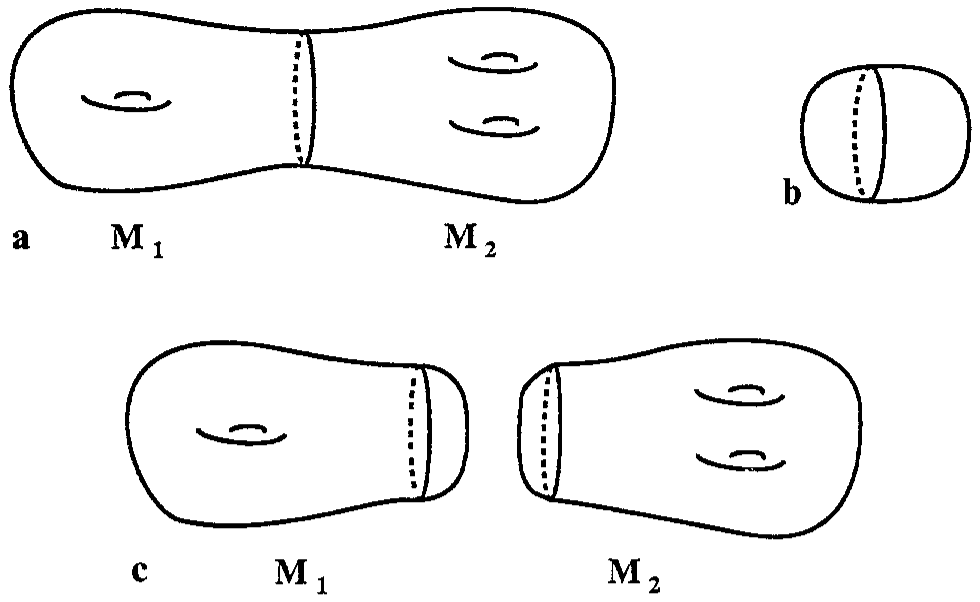
\includegraphics[width=0.68\linewidth]{figures/fig05.png}
    \caption{a 中画出的三维流形 $M$ 是两片 $M_1$ 与 $M_2$ 沿球面 $S^2$ 粘成的连通和。类似地，三维球面 $S^3$ 可沿其赤道切开（b）。按 a、b 所示分别切开 $M$ 与 $S^3$ 后，可把各片重新排列为 $M_1$ 与 $M_2$ 的不连通并，如 c 所示。（原文 p.~375，Fig.~5）}
\end{figure}

同样地，在图 5a 的右边，我们看到一个三维流形 $M_2$，其边界是同一个 $S^2$ 但定向相反；
它的希尔伯特空间 $\mathcal{H}'$ 典范地是 $\mathcal{H}$ 的对偶。$M_2$ 上的路径积分确定
$\mathcal{H}'$ 中的一个向量 $\psi$；按量子场论的一般思想，连通和 $M$ 的配分函数为
\begin{equation}
    Z(M)=(\chi,\psi).
    \tag{4.3}
\end{equation}

符号 $(\chi,\psi)$ 表示向量 $\chi\in\mathcal{H}$、$\psi\in\mathcal{H}'$ 的自然配对。
我们无法计算 (4.3)，因为既不知道 $\chi$ 也不知道 $\psi$。不妨考虑这个主题的一些变体。
把图 5a 中隔开两部分的那个二维球面 $S^2$ 嵌入 $S^3$，可以令 $S^3$ 被分成两个三维球
$B_L$ 与 $B_R$。$B_L$ 与 $B_R$ 上的路径积分会在 $\mathcal{H}$ 与 $\mathcal{H}'$ 中分别
给出向量 $v$ 与 $v'$，而导致 (4.3) 的同样推理给出
\begin{equation}
    Z(S^3)=(v,v').
    \tag{4.4}
\end{equation}

同样，我们不知道 $v$ 与 $v'$，无法计算 (4.4)。但可以作如下论断：由于 $\mathcal{H}$ 是
一维的，$v$ 必是 $\chi$ 的倍数；同样，由于 $\mathcal{H}'$ 是一维的，$v'$ 必是 $\psi$ 的
倍数。于是由一维线性代数立得
\begin{equation}
    (\chi,\psi)\cdot(v,v')=(\chi,v')\cdot(v,\psi).
    \tag{4.5}
\end{equation}
(4.5) 右端的两个量分别是 $Z(M_1)$ 与 $Z(M_2)$，如图 5c 所示。因此 (4.5) 等价于所要
证明的结果 (4.1)。

% [Tutor Note: 方法——切割-粘贴是 §4 全部计算的骨架] 这一段论证只用了三件东西：$S^2$ 上的
% 希尔伯特空间一维（上文特例 (i)）；切开的流形给出边界态向量；闭流形的配分函数是配对。
% 后面所有显式计算都是同一手法的重复：把 $S^3$ 中的链环拆成一个个圆圈再逐个接回（(4.6)
% 起的“链环连通和”），或把三维流形沿环面切成两部分、再用模变换重新展开边界态（手术公式）。
% 注意 (4.5) 的成立**只因为** $\mathcal{H}$ 与 $\mathcal{H}'$ 都是一维的：此时矩阵元
% $(\chi,\psi)$ 不依赖于基的选取；若维数大于 1，(4.5) 这样的标量恒等式就要换成矩阵乘积，
% 切割-粘贴给出的是矩阵元或其迹，而不是可以直接消去的数——这正是后文处理环面边界时改用
% S 矩阵、T 矩阵的原因。

人们或许会问：(4.1) 中如此显眼的那个神秘对象 $Z(S^3)$ 究竟是什么？能否把它设为一？
事实上，量子场论的公理足够强，$Z(S^3)$ 的值是唯一确定的，不能任意假设；后文将看到，
它可以从仿射李代数的理论算出。对 $G=SU(2)$，其公式已在 (2.26) 中给出。

% [Tutor Note: 含糊处——$Z(S^3)$ 为何不能任意设定] 作者说 $Z(S^3)$ 由量子场论公理唯一确定，
% 却未在此给出论证。要点是：$S^3=B_L\cup_{S^2}B_R$，而 $B^3$ 的路径积分给出
% $\mathcal{H}(S^2)=\mathbb{C}$ 中的真空向量 $v$，故 $Z(S^3)=(v,v)$ 就是 $v$ 的模方；这个
% 模方并非自由的归一化常数，而由路径积分测度（等价地由能级移动 $k+h^\vee$ 与 $k$ 的整性
% 条件）唯一固定。后文 (4.38) 将证明 $Z(S^3)=S_{00}$，而 $S_{00}$ 由仿射李代数给出
% （$SU(2)$ 即 (2.26)，其大 $k$ 行为 $Z\sim k^{-3/2}$ 正比于平凡联络的“负形式维数”，见 §2
% 中 (2.26) 之后的讨论及该式的脚注）。

作为 (4.1) 的一个特例，取 $G$ 的 $s$ 个不可约表示，记为 $R_1,\ldots,R_s$，并考虑 $S^3$
中由 $s$ 个互不链接、也不打结的圆圈 $C_i$ 所构成的链环。

% （原文此句在印刷页 375 底部以 “with” 截断，后续内容见 PDF p.26，由 s06 片段接续；
%   本片段到此为止，不包含 p.26 的任何正文、图注与公式。）


% =============================================================================
%  §4.1 三维球面中的纽结（上）
%  覆盖：PDF p.26 页首 – p.31 末；印刷页 376–381
%  编号公式：(4.6)–(4.19)（其中 (4.6)(4.7) 属于 §4 开头论证的续篇，
%            位于 "4.1. Knots in S^3" 标题之前，故置于 \subsection 之前）
%  插图标记：FIG 6（p.26）、FIG 7（p.27）、FIG 8/9/10（p.29）、FIG 11（p.31）
% =============================================================================

% ---------------------------------------------------------------------------
%  PDF p.26 页首（承接 p.25 末句："…consists of s unlinked and unknotted
%  circles C_i, with"；本段属 §4 开头，不属于 4.1）
% ---------------------------------------------------------------------------

每个圈各配以其中一个 $R_i$。这一点已在图 6 中标明。
\begin{figure}[htbp]
    \centering
    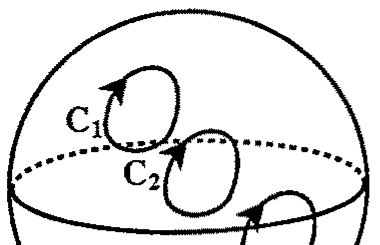
\includegraphics[width=0.26\linewidth]{figures/fig06.png}
    \caption{一个三维球面，其上画有 3 个互不链接、且各自平凡（unknotted）的圆圈 $C_i$，分别与表示 $R_1,\dots,R_3$ 相联系。该图可用多种方式切开，以把这些圆圈彼此分开。（原文 p.~376，Fig.~6）}
\end{figure}

把 $S^3$ 上带这组威尔逊线的配分函数记为 $Z(S^3;C_1,\dots,C_s)$（其中各表示 $R_i$ 均已默认给定）。于是，把图形切开、使各个圈彼此分离，并反复使用式 (4.1)，我们得知
\begin{equation}
    \frac{Z(S^3;C_1,\dots,C_s)}{Z(S^3)}
    = \prod_{k=1}^{s}\frac{Z(S^3;C_k)}{Z(S^3)}\,.
    \tag{4.6}
\end{equation}
若引入链环 $L$ 的归一化期望值，定义为 $\langle L\rangle=Z(S^3;L)/Z(S^3)$，则式 (4.6) 变为
\begin{equation}
    \langle C_1\dots C_s\rangle = \prod_{k}\langle C_k\rangle
    \tag{4.7}
\end{equation}
其中 $C_1,\dots,C_s$ 是 $S^3$ 上任一组互不链接、也不打结的威尔逊线。

% [Tutor Note: 归一化与乘性（式 (4.1)、(4.6)、(4.7)，印刷 p.375–376）。式 (4.1) 是沿 $S^2$ 的连通和公式 Z(M₁#M₂)/Z(S³)=[Z(M₁)/Z(S³)]·[Z(M₂)/Z(S³)]，其证明只用到一点：$S^2$ 上的物理希尔伯特空间是一维的，因而配分函数可以写成两个向量配对之积与一个公共因子的乘积（见印刷 p.375 式 (4.3)–(4.5)）。把该论证沿 s 个圈逐个重复，就得到 (4.6)。两处易错：(i) $Z(S^3)$ 不能随手设为 1——它由理论本身唯一决定（$G=SU(2)$ 时见式 (2.26)），只有比值 $Z(S^3;L)/Z(S^3)$ 才充当链环不变量；(ii) (4.6) 的乘积要求 s 个圈两两互不链接，且分子中第 k 个圈所带的表示必须与因子 $Z(S^3;C_k)$ 中的表示一致（原文 "the representations $R_i$ being understood"）。一旦圈之间有链接，切割所得的中间态不再唯一，乘积公式即失效。]

纽结理论中还有另一种连通和的概念，即“链环的连通和”。Jones 不变量在这一运算之下也具有简单的乘性行为；我们将在 §4.5 末尾对此作一简要说明。

\subsection{三维球面中的纽结}
% （本节重点见 §4 开头片段）

下面我们将说明“拆接关系”（skein relation）的来源；对 $S^3$ 上的纽结而言，这一关系可以取作纽结多项式的定义。（拆接关系的一个特例最早由 Conway 在讨论 Alexander 多项式时使用。）

考虑一般三维流形 $M$ 上的一个链环 $L$，如图 7a 所示。链环的各个分支带有 $G$ 的某些表示，我们希望计算式 (1.6) 所给出的费曼路径积分，以下记作 $Z(L)$（相应的表示已默认给定）。我们将通过推出一个“解纽结”的算法来计算它。如果图 7 中的线条能够彼此毫无阻碍地穿过，那么所有纽结都能被解开。实际情况并非如此：某些不走运的交叉妨碍了这一点，例如图中用圆圈圈出的那个交叉。让我们围绕这个交叉作一个小球面，把它挖出来，再仔细研究。这样就把 $M$ 切成两块；重新排列之后如图 7b 所示：图的左边是复杂的一块 $M_L$，右边是简单的一块 $M_R$。$M_R$ 是一个以 $S^2$ 为边界的三维球体；在这个边界上有四个标记点，它们在球体内部由两条线相连。

为使讨论具体化，设规范群为 $G=SU(N)$，并设所有威尔逊线都取 $SU(N)$ 的定义 $N$ 维表示，我们把这个表示记作 $R$。于是，正如我们在上一节末尾所看到的，与 $M_L$、$M_R$ 的边界相联系的物理希尔伯特空间 $\mathcal{H}_L$ 与 $\mathcal{H}_R$ 都是二维的。
\begin{figure}[htbp]
    \centering
    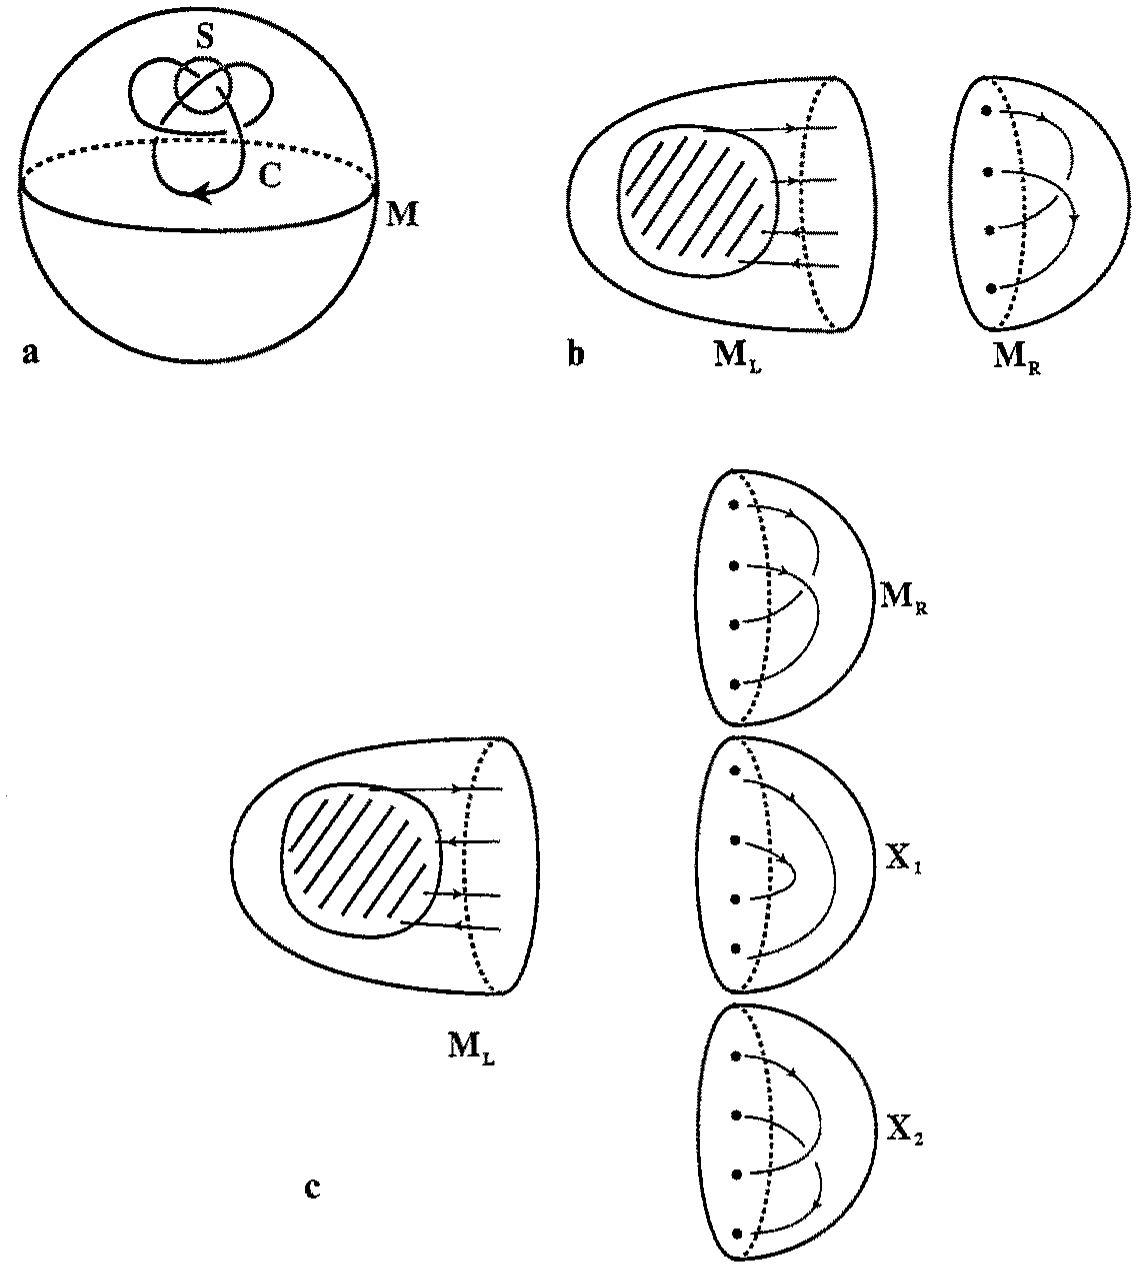
\includegraphics[width=0.79\linewidth]{figures/fig07.png}
    \caption{a 中画出一股一般三维流形 $M$ 上的链环 $C$；围绕一个“不便”的交叉画出小球面 $S$，它把 $M$ 切成简单的一片（$S$ 的内部）与复杂的一片。b 中把图重新排列，以更清楚地显示 $M$ 的切割：两片分别出现在左右两侧，即 $M_L$（细节未画出的复杂片）与 $M_R$（$S$ 的内部）。拆接关系（skein relation）的关键在于考虑用某些替代物替换 $M_R$，如 c 所示。（原文 p.~377，Fig.~7）}
\end{figure}

现在的策略与导致乘性关系 (4.1) 的策略完全相同：$M_L$ 上的费曼路径积分确定 $\mathcal{H}_L$ 中的一个向量 $\chi$，$M_R$ 上的费曼路径积分确定 $\mathcal{H}_R$ 中的一个向量 $\psi$。向量空间 $\mathcal{H}_L$ 与 $\mathcal{H}_R$（它们联系于同一个黎曼面 $S^2$，但定向相反）互为典范对偶，而配分函数即费曼路径积分 $Z(L)$ 等于它们的自然配对
\begin{equation}
    Z(L) = (\chi,\psi)\,.
    \tag{4.8}
\end{equation}
我们无法计算 (4.8)，因为 $\chi$ 与 $\psi$ 我们都不知道。目前我们唯一知道的是：（对于所考虑的群与表示）这个配对发生在一个二维向量空间之中。二维向量空间有一个绝妙的性质：任意三个向量都满足一个线性相关关系。因此，给定 $\mathcal{H}_R$ 中任意另外两个向量 $\psi_1$ 与 $\psi_2$，就必有一个线性关系
\begin{equation}
    \alpha\psi + \beta\psi_1 + \gamma\psi_2 = 0\,,
    \tag{4.9}
\end{equation}
其中 $\alpha$、$\beta$、$\gamma$ 为复数。

% [Tutor Note: Wilson 圈期望值与链环不变量（式 (4.8)，印刷 p.377）。切割–粘贴论证表明 $Z(L)$ 只依赖于链环（带标架地）嵌入 $M$ 的拓扑方式，而不依赖度规或联络 $A$ 的具体选取，这正是“拓扑场论”的含义。但要强调：$W_R(C)=\mathrm{Tr}_R P\exp\int_C A\,\mathrm{d}x$ 需要沿 $C$ 的一个法标架（framing）才能良定义——正规化自环绕数时用到了它（见印刷 p.380 的 "Change of Framing" 一段）。所以严格说 $Z(L)$ 是“带标架链环”的不变量，只有去掉标架依赖才得到通常的纽结多项式。下文 (4.13)–(4.19) 中所有 $\alpha,\beta,\gamma$ 的数值都携带这一约定，切勿与文献中“标准标架”下的数值直接混用。]

物理上，有一个非常自然的办法在 $\mathcal{H}_R$ 中得到新的向量。如果把图 7b 中的 $M_R$ 换成任何一个具有相同边界的其他三维流形 $X$（并在 $X$ 内用适当的弦连接 $M_R$ 边界上的那些标记点），那么 $X$ 上的费曼路径积分就给出 $\mathcal{H}_R$ 中的一个新向量。为这一计算任取两个方便的三维流形 $X_1$ 与 $X_2$，就得到可用于 (4.9) 的向量 $\psi_1$ 与 $\psi_2$。我们将考虑这样的情形：$X_1$ 与 $X_2$ 与 $M_R$ 是同一个流形，只是把边界上各点连起来的“辫”不同；这一点如图 7c 所示。

一旦以这种方式得到 $\psi_1$ 与 $\psi_2$，式 (4.9) 便有显然的推论
\begin{equation}
    \alpha(\chi,\psi) + \beta(\chi,\psi_1) + \gamma(\chi,\psi_2) = 0\,.
    \tag{4.10}
\end{equation}
式 (4.10) 中的三项有一个“物理”解释，这在图 7c 中一目了然。把 $M_L$ 与 $M_R$ 或其替代者 $X_1$、$X_2$ 重新粘合起来，就还原出原来的三维流形 $M$，只是原来的链环 $L$ 被某些新的链环所代替。因此，(4.10) 就等价于所关心的那些链环期望值之间的一个关系，即
\begin{equation}
    \alpha Z(L) + \beta Z(L_1) + \gamma Z(L_2) = 0\,.
    \tag{4.11}
\end{equation}
这个递推关系常被画成图 8 的样子。该图的含义如下：若考虑三个链环，它们的平面投影在一个圆盘之外完全相同，而在该圆盘之内恰好是图中三个画法之一，那么这三个链环的期望值分别以 $\alpha$、$\beta$、$\gamma$ 为系数加权之后，相加为零。

% [Tutor Note: 拆接关系 (4.11) 的场论来源（印刷 p.378）。它并不是一条组合学的假设，而是“$\mathcal{H}_R$ 是二维的”这一事实的线性代数后果：$S^2$ 上带 4 个标记点的共形块空间维数为 2（$SU(N)_k$ 中 $R\otimes R$ 只有对称与反对称两个融合道，即后文的 $E_1$、$E_2$），故 $\psi,\psi_1,\psi_2$ 必然线性相关。系数 $\alpha,\beta,\gamma$ 只依赖 $G,k$ 与各分支所带的表示，与具体链环无关——这正是“普适性”（universality）的来源。Witten 的新意在于：在 Conway/Jones 的框架里，类似 (4.11) 的关系只能作为公理、定义或经验规则引入，而这里它是三维拓扑场论的一条定理，因而自洽性自动得到保证（见印刷 p.379 末–380 首的讨论）。此处最容易被误读成“只是图形技巧”，务必抓住唯一输入：二维希尔伯特空间。]

纽结理论中众所周知，(4.11) 唯一地决定了 $S^3$ 中所有纽结的期望值。为方便起见，我们给出一个简短的说明。我们从纽结的一个平面投影出发，如图 9 所示。交叉数 $p$ 是有限的。归纳地假设：所有交叉数不超过 $p-1$ 的纽结，其期望值都已算得。现在要研究有 $p$ 个交叉的纽结。如果在 (4.11) 中 $\beta=0$，那么在每个交叉处都可以把两条线股互相穿过，只需在把上交叉换成下交叉时带上一个因子 $-\gamma/\alpha$。倘若如此，这些线实际上就是“透明”的，所有纽结都能被解开。实际情况是 $\beta\neq 0$，但正比于 $\beta$ 的那一项会减少交叉数，从而给出一个新的链环，而它的期望值已由归纳假设知道。

这一过程把讨论归结到 $p=0$ 的情形：此时没有交叉，因而我们只与若干个互不链接、也不打结的圈打交道。为了练习使用 (4.11)，让我们明确讨论这一情形。在图 10 中我们画出了图 8 的一个有用的特例。图 10 中的第一个和第三个链环都由一个不打结的圈构成，第二个则由两个互不链接、不打结的圈构成。
\begin{figure}[htbp]
    \centering
    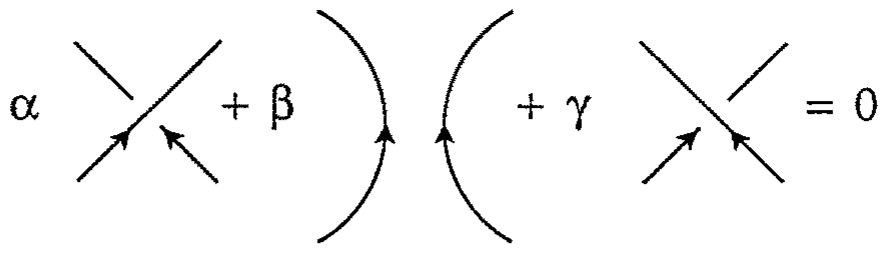
\includegraphics[width=0.61\linewidth]{figures/fig08.png}
    \caption{链环的一个递归关系。（原文 p.~379，Fig.~8）}
\end{figure}
\begin{figure}[htbp]
    \centering
    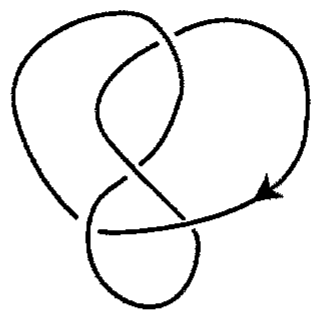
\includegraphics[width=0.25\linewidth]{figures/fig09.png}
    \caption{一个纽结的平面投影，含四个交叉。（原文 p.~379，Fig.~9）}
\end{figure}
\begin{figure}[htbp]
    \centering
    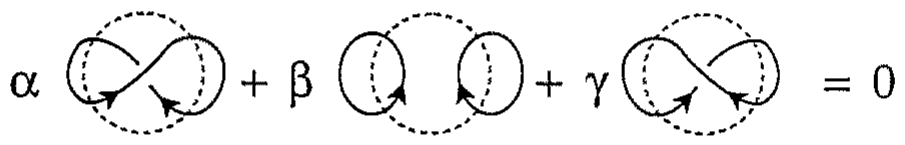
\includegraphics[width=0.62\linewidth]{figures/fig10.png}
    \caption{图 8 用法的一个特例：三幅图在虚线之外完全相同，在虚线之内则形如图 (4.11)。（原文 p.~379，Fig.~10）}
\end{figure}
设 $N$ 维表示下 $s$ 个互不链接、不打结的圈在 $S^3$ 上的配分函数为 $Z(S^3;C_s)$，那么在这一情形下 (4.11) 就归结为如下断言：
\begin{equation}
    (\alpha+\gamma)\,Z(S^3;C) + \beta Z(S^3;C^2) = 0\,.
    \tag{4.12}
\end{equation}
结合 (4.7)\footnote{这是唯一必须用到 (4.7) 的地方。上一段中的归纳不借助 (4.7) 就把 $S^3$ 中纽结的一切计算归结为这一特例。}，便可推出：$SU(N)$ 的 $N$ 维表示中一个不打结的威尔逊线的期望值为
\begin{equation}
    \langle C\rangle = -\frac{\alpha+\gamma}{\beta}\,.
    \tag{4.13}
\end{equation}

% [Tutor Note: 记号陷阱与符号（式 (4.12)、(4.13)，印刷 p.379）。关键：$Z(S^3;C_s)$ 中的下标 s 指“圈的个数”，不是“第 s 个圈”（原文 "the partition function for s unlinked and unknotted circles ... as Z(S³; C_s)"）。因此 (4.12) 中 $Z(S^3;C)$ 对应 $s=1$、$Z(S^3;C^2)$ 对应 $s=2$（两个互不链接、不打结的圈）；而 $Z(S^3;C^2)=Z(S^3;C)^2/Z(S^3)$ 正是 (4.7) 在 $s=2$ 时的内容，不先动用 (4.7) 无法从 (4.12) 解出 (4.13)。另注意 (4.13) 的整体符号为负：$\beta\to 0$ 时它发散，正对应上文“若 $\beta=0$ 则可解开一切纽结”这一图像。]

% [Tutor Note: 原文笔误（印刷 p.378 末段，PDF p.28）："The first and third links in links in Fig. 10" 中 "in links in" 系重复，应为 "The first and third links in Fig. 10"。译文按正确语义处理，特此标明。]

现在我们把这个公式完全明确化，即用基本量子场论参数 $N$ 与 $k$ 把 $\alpha$、$\beta$、$\gamma$ 算出来。

上述归纳表明：任何纽结的期望值都可以在有限多步之后表示为 $\alpha$、$\beta$、$\gamma$ 的有理函数（两个多项式之比）。正是在这个意义上，Jones 纽结不变量及其各种推广才是“多项式”。正如我们已看到的，证明 (4.11) 唯一决定纽结不变量相对来说是初等的，但反过来远不那么显然。(4.11) 可以用许多不同的方式去求某个给定链环的期望值，因此必须证明这样做不会遇到任何不自洽之处。虽然这一点已用多种方法证明，但这些证明都不是内蕴三维的——(4.11) 此前从未从一个明显不变的三维框架中导出。这正是本讨论的新颖之处。

\textbf{标架的改变（Change of Framing）。}我们想计算 $\alpha$、$\beta$、$\gamma$，但作为准备，必须先讨论一个技术要点。在 §2 末尾我们得知：选定一个圈 $C$ 与一个表示 $R$，并不足以给出良定义的量子和乐算符 $W_R(C)=\mathrm{Tr}_R\,P\exp\int_C A\,\mathrm{d}x$。还必须为圈 $C$ 选一个“标架”（framing）；当需要计算 $C$ 的自环绕数及其非阿贝尔与量子的推广时，标架就会介入。在 §2 末尾，我们曾许诺推导出一个公式 (2.33)，说明任何插入了 $W_R(C)$ 的配分函数在标架改变下如何变换。现在是兑现这一许诺的时候了。

% [Tutor Note: 标架与共形权（印刷 p.380）。$t$ 重 Dehn 扭转是边界黎曼面 $\Sigma$ 上的一种映射类（modular）变换，它在 $\mathcal{H}_R$ 上实现为乘以 $e^{2\pi i t h_R}$；几何上，它把圈 $C$ 的标架平移 $t$ 个单位（自环绕数改变 $t$），于是“插入 $W_R(C)$ 的配分函数”按 $e^{2\pi i t h_R}$ 变换。这正是“标架反常”的场论表述：$h_R$ 就是表示 $R$ 的初级场的共形权。易错处：(i) 指数中是 $h_R$ 而非中心荷 $c$；(ii) 本文的 $k$ 是陈–西蒙斯作用量 (1.3)（即 $\frac{k}{4\pi}\int_M\mathrm{Tr}(A\wedge\mathrm{d}A+\frac{2}{3}A^3)$）中的能级，与之对应的 WZW 能级是 $k+N$，故 $h_R=(N^2-1)/(2N(N+k))$（脚注 11）；若按“把能级平移为 $k+N$”的文献记法，公式中的 $N+k$ 应换写成该平移后的能级 $k+h^\vee$（$SU(N)$ 时 $h^\vee=N$），否则分母中的能级会少算 $N$。]

如图 7b 那样，让我们沿一个与 $C$ 相交于点 $P$ 的黎曼面 $\Sigma$ 把三维流形 $M$ 切开（$\Sigma$ 或许还与其他某些点相交，但那些点无关紧要）。在之前的论证中，我们用到：与 $M_L$ 或 $M_R$ 的边界相联系的是希尔伯特空间 $\mathcal{H}_L$ 与 $\mathcal{H}_R$。此外，$\mathcal{H}_R$（例如）是“模空间上的一个平坦丛”，因此边界 $\Sigma$ 的映射类群自然地作用在 $\mathcal{H}_R$ 上。我们希望在对图 7b 的各块重新粘合之前，先以某个非常特殊的微分同胚作用在 $M_R$ 的边界上。我们要选的微分同胚，是绕 $\Sigma$ 上点 $P$ 的 $t$ 重“Dehn 扭转”（Dehn twist）。作此微分同胚，再把图 7b 的各块重新粘合起来，得到的图景看起来完全相同，但圈 $C$ 的标架已经平移了 $t$ 个单位。另一方面，在共形场论中人们知道 Dehn 扭转如何作用于 $\mathcal{H}_R$：与表示 $R$ 相联系有一个数 $h_R$，即“$R$ 表示中初级场的共形权”，而 $t$ 重 Dehn 扭转在 $\mathcal{H}_R$ 上的作用是乘以 $e^{2\pi i t h_R}$。这样我们就得到了 (2.33)，其中 $h=h_R$。

\textbf{显式计算（Explicit Evaluation）。}现在我们来确定关键方程 (4.10) 中出现的参数 $\alpha$、$\beta$、$\gamma$。这需要确定图 7c 中三个向量 $\psi$、$\psi_1$、$\psi_2$ 之间的显式关系，而这又要求进一步研究一个二维希尔伯特空间：它作为 $S^2$ 上 $R,R,\bar R,\bar R$ 四点函数的共形块空间而出现［这里 $R$ 就是 $SU(N)$ 的定义 $N$ 维表示，$\bar R$ 是其对偶表示］。图 7c 中的三种位形可以看作彼此相差 $S^2$ 的某个微分同胚；这个微分同胚就是“半单值性”（half-monodromy）：两份 $R$ 互相绕行半圈而交换位置，如图 11 所示。Moore 与 Seiberg 称这一操作为 $B$，并对它作了广泛研究。态 $\psi_1$ 与 $\psi_2$ 正是
\begin{equation}
    \psi_1 = B\psi\,,\qquad \psi_2 = B^2\psi\,.
    \tag{4.14}
\end{equation}
矩阵 $B$ 作用在二维空间中，因此满足一个特征方程
\begin{equation}
    B^2 - y B + z = 0\,,
    \tag{4.15}
\end{equation}
\begin{figure}[htbp]
    \centering
    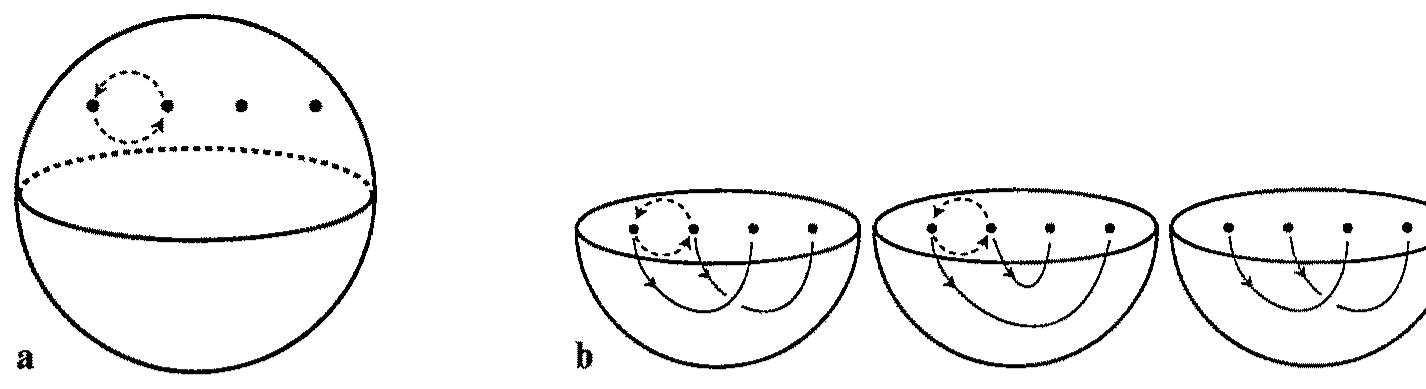
\includegraphics[width=0.98\linewidth]{figures/fig11.png}
    \caption{a 中画出交换 $S^2$ 上两个等价点的“半单值”（half-monodromy）操作；箭头示意前两个点绕彼此做半扭转而交换位置。b 的意思是：若第一幅图中左侧两点绕彼此做半扭转，则第一幅图变为第二幅；再做一次，第二幅变为第三幅。图 7c 右侧的三幅图正是通过一连串半单值操作相互联系的。（原文 p.~381，Fig.~11）}
\end{figure}
其中
\begin{equation}
    y = \mathrm{Tr}\,B\,,\qquad z = \det B\,.
    \tag{4.16}
\end{equation}
由 (4.14) 可见，$\psi$、$\psi_1$、$\psi_2$ 之间的线性关系（只差一个无关紧要的公共因子）就是
\begin{equation}
    z\cdot\psi - y\cdot\psi_1 + \psi_2 = 0\,,
    \tag{4.17}
\end{equation}
而根据 (4.16)，要使它显式化，我们只需知道 $B$ 的本征值（从而知道其行列式与迹）。

% [Tutor Note: 辫群表示的迹与 $B$ 矩阵（式 (4.14)–(4.17)，印刷 p.380–381）。$\psi_1=B\psi$、$\psi_2=B^2\psi$ 中的 $B$ 是半单值化，Moore–Seiberg [13] 对它作了系统研究；在二维空间中由 Cayley–Hamilton 定理得 (4.15)，于是 $B^2=yB-z$，作用到 $\psi$ 上即 $\psi_2=y\psi_1-z\psi$，移项便是 (4.17)。对照 (4.9) 可知 $(\alpha,\beta,\gamma)$ 与 $(z,-y,1)$ 成比例——$B$ 的迹 $y$ 与行列式 $z$ 只决定拆接系数之比，$\alpha,\beta,\gamma$ 的绝对标度另有约定（见 (4.20) 后的公共因子）。此处有两处符号/字形陷阱：(i) (4.15) 中 $yB$ 前是负号，即 $B^2=yB-z$，切勿写成 $B^2+z=yB$ 后在 (4.17) 中错号；(ii) 字形陷阱格外要紧：$y=\mathrm{Tr}\,B$ 是斜体拉丁字母 $y$（印刷 p.381 式 (4.15)–(4.17) 清楚印作 $y$），而拆接系数是希腊字母 $\gamma$（(4.9)、(4.11)–(4.13)、(4.20)），二者是两个不同的量；OCR 把正文的 $\gamma$ 抽成“7”、把公式里的 $y$ 抽成“y”，极易混同。自检：由 (4.19)，$|\mathrm{Tr}\,B|$ 一般不等于 $1$（例如 $N=2$、$k=1$ 时 $\lambda_1=e^{-i\pi/6}$、$\lambda_2=-i$，故 $|\mathrm{Tr}\,B|=\sqrt3$），而 (4.20) 的 $\gamma$ 是模为 $1$ 的相位，所以 (4.15)–(4.17) 中的字母只能是 $y$，不能是 $\gamma$。]

这些本征值可从 [13] 得到，但在叙述具体公式之前，我想指出一个重要的微妙之处。正如我们在上一个小节中讨论过的，一切具体结果，例如 $\alpha$、$\beta$、$\gamma$ 的数值，都依赖纽结的标架。在任意三维流形上工作时最自然的约定，并不是讨论 $S^3$ 上纽结时通常采用的约定。

在研究图 7c 时，要描述相对标架，任务在于确定右边三幅图之间的相对标架，因为左边那幅图是固定不动的。如果只看这三幅图而忽略线条不能彼此穿过这一事实，那么在一种显然的意义上，人们会愿意为每幅图取“同一个”标架；例如，一个垂直穿出纸面的单位向量就在图中每个链环上定义了一个法向量场。这与 Moore 和 Seiberg 在定义 $B$ 的本征值时所取的约定等价，因此我们现在可以直接引用他们的结果。设 $h_R$ 是变换为 $R$ 的初级共形场的共形权，$E_i$ 是 $SU(N)$ 在 $R\otimes R$ 分解中出现的不可约表示，$h_{E_i}$ 是对应初级场的权。则 $B$ 的本征值为
\begin{equation}
    \lambda_i = \pm\exp\bigl(i\pi(2h_R - h_{E_i})\bigr)\,,
    \tag{4.18}
\end{equation}
其中 $+$ 或 $-$ 号取决于 $E_i$ 在 $R\otimes R$ 中是按对称方式还是按反对称方式出现。若 $R$ 是 $SU(N)$ 的 $N$ 维表示，则可得\footnote{对此表示，$h_R=(N^2-1)/\bigl(2N(N+k)\bigr)$。在 $R\otimes R$ 的分解中，对称部分是一个不可约表示，其 $h_{E_1}=(N^2+N-2)/\bigl(N(N+k)\bigr)$；反对称部分是一个不可约表示，其 $h_{E_2}=(N^2-N-2)/\bigl(N(N+k)\bigr)$。} $B$ 的本征值为
\begin{equation}
    \lambda_1 = \exp\biggl(\frac{i\pi(-N+1)}{N(N+k)}\biggr)\,,
    \qquad
    \lambda_2 = -\exp\biggl(\frac{i\pi(N+1)}{N(N+k)}\biggr)\,.
    \tag{4.19}
\end{equation}

% [Tutor Note: $R$ 矩阵与量子群（式 (4.18)、(4.19)，印刷 p.381）。$\lambda_i=\pm\exp(i\pi(2h_R-h_{E_i}))$ 正是量子群 $U_q(\mathfrak{su}(N))$ 的 $R$ 矩阵在 $R\otimes R$ 上的两个本征值，$q=e^{2\pi i/(N+k)}$（见印刷 p.382 式 (4.21)）；$\pm$ 号对应 $E_i$ 在 $R\otimes R$ 中对称/反对称出现，即两个融合道 $E_1$、$E_2$。指数的来历是：两份 $R$ 互换位置相当于各绕行半圈，给出因子 $\exp(i\pi\cdot 2h_R)$ 与 $\exp(-i\pi h_{E_i})$ 之积；两次这样的半单值性合成一次完整绕行，相位为 $e^{2\pi i(2h_R-h_{E_i})}$，故半单值性的本征值是它的平方根（参见印刷 p.381 Fig. 11 的说明）。可用脚注 11 的三条 $h$ 值自检 (4.19)：$2h_R-h_{E_1}=(1-N)/\bigl(N(N+k)\bigr)$ 给出 $\lambda_1$，$2h_R-h_{E_2}=(N+1)/\bigl(N(N+k)\bigr)$ 给出 $\lambda_2$，符号与对称/反对称对应关系一致。]


% =============================================================================
%  s07-calculability-b.tex
%  §4.1 收尾（PDF p.32 页首，印刷 p.382）、§4.2 链环上的手术（p.33–34，383–384）、
%  §4.3 亏格一情形的物理希尔伯特空间（p.34–36，384–386）、
%  §4.4 $S^1\times X$ 上的路径积分（p.37，387）
%  编号公式：(4.20)–(4.32)。（(4.16)–(4.19) 在 p.30–31，不属本片段。）
%  插图标记：Fig. 12（p.33 首见；p.34–36 引用）、Fig. 13（p.34）、Fig. 14（p.37）
% =============================================================================

% （4.1 节续）
把这些公式代入式 (4.16)、(4.17)，就能把我们前面的结果完全显式化；这一步是直接的。

在把这些结果与纽结理论文献作比较之前，必须先作一处修正。对于 $S^3$ 中的链环，
总存在一个标准标架（standard framing），使得链环每个分支的自相交数
（self-intersection number）为零。文献中引用 $S^3$ 中纽结的多项式取值时，
通常并不指明标架；这些取值就是取标准标架的链环的取值。然而，如果在图 7c 的右侧
对每一幅图都使用“相同”的标架，那么把图 7c 的右侧粘到左侧上时，
每个链环就不再具有典范标架（canonical framing）了。若第一个纽结按标准方式取标架，
则第二个纽结的标架相差一个单位，第三个相差两个单位。因此，在用式 (4.19) 算出
$\alpha,\beta,\gamma$ 之后，若要和纽结理论文献的约定一致，我们还必须把 $\beta$
乘以 $\exp(-2\pi i h_R)$、把 $\gamma$ 乘以 $\exp(-4\pi i h_R)$。作了这些修正之后，
得到

\begin{gather}
    \alpha = -\exp\left(\frac{2\pi i}{N(N+k)}\right), \notag \\
    \beta = -\exp\left(\frac{i\pi(2-N-N^2)}{N(N+k)}\right)
            +\exp\left(\frac{i\pi(2+N-N^2)}{N(N+k)}\right), \tag{4.20} \\
    \gamma = \exp\left(\frac{2\pi i(1-N^2)}{N(N+k)}\right). \notag
\end{gather}

% [Tutor Note: 标架与整体反常] 上面这段“修正”是全文最容易读漏、也最容易算错的地方。
% $S^3$ 中的链环有标准标架（沿 Seifert 曲面法向取定的零标架），此时每个分支的自相交数
% （等于该分支的自环绕数、也就是它的标架数）为零，而文献中的纽结多项式默认取的就是这一标架。
% 但图 7c 的粘合要求左右两图使用“同一个”标架：若第一个纽结取标准标架，第二个就差一个单位、
% 第三个差两个单位。对一条处于表示 $R$ 的威尔逊线，标架每改变一个单位，其振幅就乘上因子
% $\exp(2\pi i h_R)$，其中 $h_R$ 是相应初级场在能级 $k$ 下的共形权（conformal weight），
% 而不是有限维群的 Casimir。这个相位就是所谓标架反常（framing anomaly）：它来自
% 陈–西蒙斯配分函数的整体反常，其强度由中心荷决定。于是把 $\beta$ 乘 $\exp(-2\pi i h_R)$、
% 把 $\gamma$ 乘 $\exp(-4\pi i h_R)$ 正是把带错误标架的振幅改回标准标架；两个因子的指数
% 相差一倍，恰好对应两条威尔逊线的标架误差相差一个单位。核对时请务必分清 $h_R$、对偶 Coxeter 数
% $h^\vee$ 与 Casimir 三者，混用会差出含 $k$ 的多项式因子。

如果把 $\alpha,\beta,\gamma$ 同乘一个无关紧要的公共因子
$\exp\bigl(i\pi(N^2-2)/N(N+k)\bigr)$，并引入变量

\begin{equation}
    q = \exp\bigl(2\pi i/(N+k)\bigr), \tag{4.21}
\end{equation}

那么拆接关系（skein relation）可以更简洁地写成

\begin{equation}
    -q^{N/2}L_+ + \bigl(q^{1/2}-q^{-1/2}\bigr)L_0 + q^{-N/2}L_- = 0. \tag{4.22}
\end{equation}

这里 $L_+$、$L_0$、$L_-$［分别相当于式 (4.11) 中的 $L$、$L_1$、$L_2$］
是上交叉（overcrossing）、零交叉（zero crossing）与下交叉（undercrossing）的标准记号；
而对 $i=+,0,-$，今后我们直接写 $L_i$，不再写 $Z(L_i)$。式 (4.22) 的归一化是正确的，
它给出 $S^3$ 中取标准标架的纽结的正确答案；因此，如果只关心 $S^3$ 中的纽结，
就可以放心使用它，完全不必去考虑标架问题。

最后，比较式 (4.13) 与式 (4.22) 可知：$S^3$ 中一条不打结的威尔逊线，
在其标准标架下的期望值为

\begin{equation}
    \langle C\rangle = \frac{q^{N/2}-q^{-N/2}}{q^{1/2}-q^{-1/2}}. \tag{4.23}
\end{equation}

% [Tutor Note: 约定与检验] 式 (4.21) 取 $q=\exp(2\pi i/(N+k))$ 是本文的关键约定：
% $N$ 是表示的维数（$G=\mathrm{SU}(N)$ 的基础表示），$k$ 是陈–西蒙斯能级（取正整数）。
% 文献中常见的其他约定还有 $q=\exp(\pi i/(k+N))$、$t=q^{-1}$、$q=\exp(2\pi i/(k+N))$ 等，
% 比较公式时若不作代换，极易把 (4.22) 的幂次与符号全部弄错。请以本式的 $q$ 为准，
% 并注意 (4.22) 中 $L_+$ 的系数是 $-q^{N/2}$、$L_-$ 的系数是 $q^{-N/2}$（二者互为倒数），
% $L_0$ 的系数是 $q^{1/2}-q^{-1/2}$；(4.23) 给出的正是量子维数
% $[N]_q=(q^{N/2}-q^{-N/2})/(q^{1/2}-q^{-1/2})$。
% 译者验算：令 $v=\exp(i\pi/N(N+k))$，则 $q=v^{2N}$；把 (4.20) 的三式同乘公共因子
% $v^{N^2-2}$，恰好得到 $-q^{N/2}$、$q^{1/2}-q^{-1/2}$、$q^{-N/2}$，与 (4.22) 逐项吻合。
% 这条代数核验说明 (4.20)–(4.22) 的转录（含 $2\pm N-N^2$ 的符号）无误，可作为读者自查的模板。
% 书中的两项检验值得记住：其一是 $N,k$ 为正整数时 (4.23) 的右边为正，这由三维陈–西蒙斯
% 理论的反射正性（reflection positivity）所要求；其二是弱耦合极限 $k\to\infty$ 时
% $\langle C\rangle\to N$，即经典极限下恢复表示的维数。这两条把量子修正与经典值锁在一起。

式 (4.23) 可以接受若干有意思的检验。首先，当 $N$、$k$ 取任意正整数时，
(4.23) 的右边都是正的——这是三维陈–西蒙斯规范理论的反射正性（reflection positivity）
所要求的。其次，在 $k\to\infty$ 的弱耦合极限下，有 $\langle C\rangle\to N$。
这一点很容易解释：在弱耦合极限下，$S^3$ 上联络 $A_i$ 的涨落无关紧要，
威尔逊线的期望值趋于 $A_i=0$ 时的取值，也就是表示的维数——在本情形中即 $N$。

\subsection{链环上的手术}
% （本节重点见 §4 开头片段）

我们已经看到，$S^3$ 中任意链环的期望值都可以有效地计算出来。现在要把这一点推广到
任意三维流形上的计算。基本想法是：通过“链环上的手术”（surgery on links）这一操作，
任何三维流形都可以化归为 $S^3$；因此，只要弄清我们所研究的不变量在手术下如何变换，
就足够了。手术操作可以这样描述。先从一个三维流形 $M$ 和一条任意选定的嵌入圆周 $C$
出发。注意，起初并没有与 $C$ 相联系的威尔逊线；$C$ 只是一条数学意义上的线，
我们将在它上面施行“手术”。为此，先把 $C$ 加粗成一个“管状邻域”
（tubular neighborhood），即以 $C$ 为中心的一个实心环面。把这个实心环面挖去后，
$M$ 被分成两块；这个实心环面在图 12b 中记作 $M_R$，剩下的部分记作 $M_L$。
然后，在 $M_R$ 的边界上作一个微分同胚，再把 $M_L$ 与 $M_R$ 粘回一起，
就得到一个新的三维流形 $\tilde{M}$。

“任何三维流形都可以通过对纽结作反复手术而从 $S^3$ 得到、或化归为 $S^3$
（或任何其他指定的三维流形）”——这并不是一个很深刻的结果。然而，这样的描述远不唯一，
而且用手术描述来计算所关心的不变量往往很困难。下面我们将会看到，
本文所研究的不变量可以有效地由手术表示（surgery presentation）计算出来。

% [Tutor Note: 手术表示与 Kirby 移动] 作者说“这不是一个很深刻的结果”，指的是
% Lickorish–Wallace 定理：任何闭可定向三维流形都可以由 $S^3$ 沿一条链环作整系数手术得到
% （对链环每个分支挖去管状邻域，再用斜率为 $\pm1$ 的边界微分同胚粘回）；等价地，
% 任何三维流形都能沿纽结作反复手术而化归为 $S^3$。原文未给证明，可查
% Lickorish, \emph{Ann. of Math.} \textbf{76} (1962) 531；Wallace,
% \emph{Canad. J. Math.} \textbf{12} (1960) 431。要紧的是“手术表示远不唯一”：
% 同一流形有无穷多种“链环＋手术系数”的描述，它们之间由 Kirby 移动相联系
% （Kirby moves：把一个分支沿另一个分支滑动，以及消去或加入一对斜率相反的平凡手术），
% 见 Kirby, \emph{Invent. Math.} \textbf{45} (1978) 35。因此，任何由手术表示定义的量，
% 都必须证明与表示的选择无关——这正是 Kirby 移动的意义，也是本文这一整套方法
% 必须面对的问题：后面用 $S$ 矩阵、$T$ 矩阵的模变换性质所作的论证，实质上就是在处理
% 这类不变性。

\begin{figure}[htbp]
    \centering
    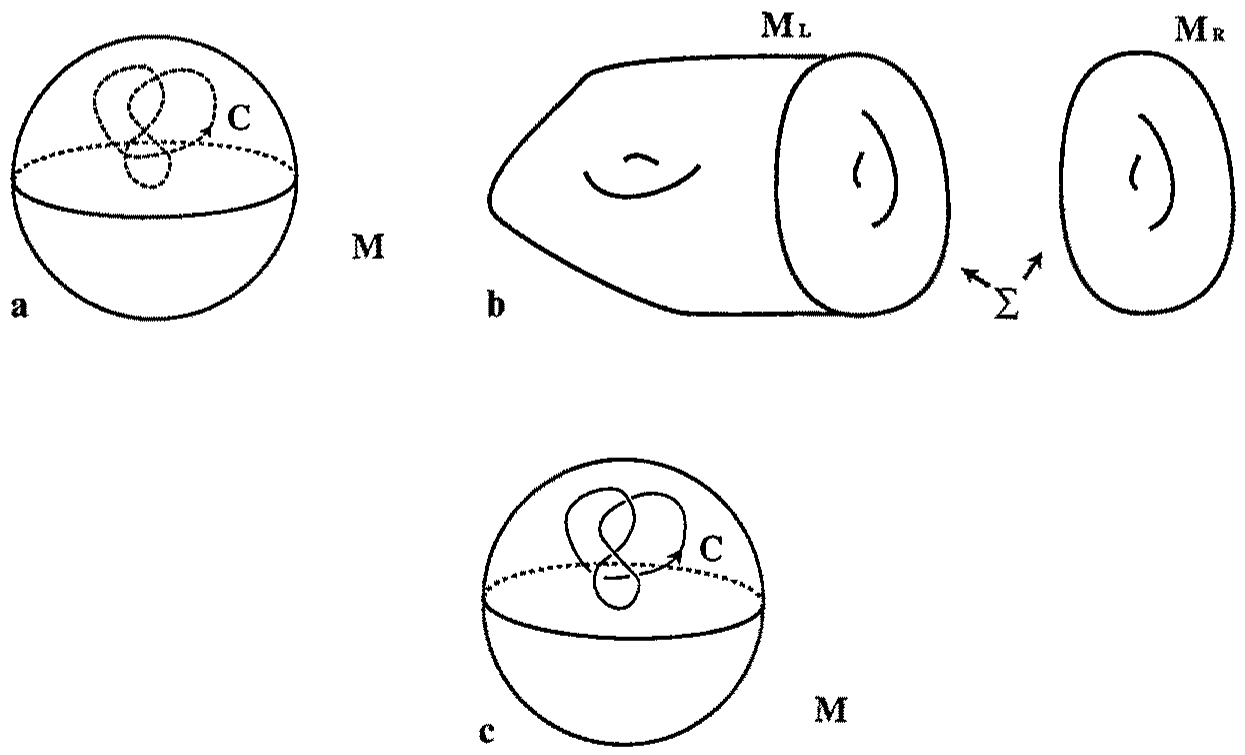
\includegraphics[width=0.86\linewidth]{figures/fig12.png}
    \caption{在三维流形 $M$ 中对圆圈 $C$ 做手术，即去掉 $C$ 的管状邻域（a）。此时 $M$ 被分成 $M_L$ 与 $M_R$ 两片，其边界是一个环面 $\Sigma$（b）。$M_R$ 就是一个实心环面；在 $M_R$ 的边界上做一次微分同胚后把两片粘回，手术即告完成。最终 $M$ 被一个新的三维流形 $\widetilde{M}$ 取代。我们随后会看到，在 $\widetilde{M}$ 上的计算等价于在 $M$ 上手术处插入一条物理威尔逊线的计算（c）。a 与 c 的差别在于：a 中 $C$ 只是手术所在的位置，而 c 中它是一条威尔逊线。（原文 p.~383，Fig.~12）}
\end{figure}

我们用标准论证来研究图 12b。与 $M_L$ 和 $M_R$ 的边界相联系的是互为典范对偶的
两个希尔伯特空间 $\mathcal{H}_L$ 与 $\mathcal{H}_R$。$M_L$ 与 $M_R$ 上的路径积分分别给出
$\mathcal{H}_L$ 与 $\mathcal{H}_R$ 中的向量 $\psi$ 与 $\chi$，而 $M$ 上的配分函数
不过是它们的自然配对 $(\psi,\chi)$。如果在把 $M_L$ 与 $M_R$ 粘回一起之前，
先用一个微分同胚 $K$ 作用在 $M_R$ 的边界上，那么 $\chi$ 就被 $K\chi$ 替换，
于是 $(\psi,\chi)$ 变成 $(\psi,K\chi)$。

% [Tutor Note: 配分函数＝边界态的配对] 这段话是 Atiyah 拓扑场论公理的具体化：对带边流形，
% 路径积分给出边界希尔伯特空间中的一个向量；把两个带边流形沿公共边界粘合，
% 配分函数就是把相应的两个向量配对。这里 $\mathcal{H}_L$ 与 $\mathcal{H}_R$ 互为典范对偶，
% 是因为边界 $\Sigma$ 在两侧的定向相反。手术＝在粘合前对边界作微分同胚 $K$，
% 配对随之变成 $(\psi,K\chi)$——这就是本节手术公式的全部内容，也是式 (4.27) 的来源。
% 请注意 $(\cdot,\cdot)$ 是 $\mathcal{H}_L\otimes\mathcal{H}_R\to\mathbb{C}$ 的自然配对，
% 并不自动是厄米内积；只有在流形具有反射正性时它才对应内积，而 (4.23) 右边的正性检验
% 用的正是这一点。

这就有可能确定该量子场论的配分函数在手术下如何变换。一旦对 $K\chi$ 有了适当理解，
我们就能把 $\tilde{M}$ 上的计算化归为 $M$ 上的计算。

\subsection{亏格一情形的物理希尔伯特空间}
% （本节重点见 §4 开头片段）

至此，我们需要亏格一情形下物理希尔伯特空间的描述。一个漂亮的描述，
恰好适合我们的需要，出现在 Verlinde 的工作 [12] 中。

首先，圈群 $LG$ 在能级 $k$ 下只有有限多个可积最高权表示。设这样的表示共有 $t$ 个。
对圈群的每一个这样的最高权表示，其最高权空间是有限维群 $G$ 的一个不可约表示。
于是出现 $t$ 个被挑出的 $G$ 表示；我们把这些表示记作 $R_0,R_1\dots R_{t-1}$，
其中 $R_0$ 表示平凡表示（它总是这张表中的一个）。Verlinde 证明：若 $\Sigma$ 是
亏格为 1 的黎曼面，则物理希尔伯特空间 $\mathcal{H}_\Sigma$ 的维数为 $t$。此外，
虽然 $\mathcal{H}_\Sigma$ 没有典范基，Verlinde 证明：$H^1(\Sigma,\mathbb{Z})$ 的每一组
由两个圈 $a$ 与 $b$ 构成的同调基的选取，都给出 $\mathcal{H}_\Sigma$ 中一组典范的基。
对我们的目的而言，这一点可以这样描述。拓扑上，把环面 $\Sigma$ 实现为某个实心环面 $U$
的边界有许多不等价的方式。$U$ 的选取可以通过要求圈 $a$ 在 $U$ 中可缩来固定。
这一点在图 13a 中作了图示。其次，对每个 $i=0\dots t-1$，按如下方式在
$\mathcal{H}_\Sigma$ 中定义一个态 $v_i$：在 $U$ 内部放置一条处于 $R_i$ 表示、
沿 $b$ 方向延伸的威尔逊线，\footnote{$U$ 边界上的 $b$ 圈给出这条威尔逊线的一个标架。}
并对 $U$ 作费曼路径积分，以此定义 $\mathcal{H}_\Sigma$ 中的向量 $v_i$。

% [Tutor Note: 亏格一维数 $t$ 的路径积分来源] 为什么 $\dim\mathcal{H}_\Sigma=t$？
% 路径积分的说法是：在环面 $\Sigma=T^2$ 上量子化陈–西蒙斯理论，得到的物理希尔伯特空间
% 正是能级 $k$ 的 WZW 模型在环面上的共形块空间；而环面上的共形块与可积最高权表示一一对应
% （每个可积表示 $R_i$ 给出一个特征标 $\chi_i(\tau)$），故维数为 $t$。这正是 Verlinde 公式
% $\dim\mathcal{H}_{\Sigma_g}=\sum_i (S_{0i})^{2-2g}$ 在 $g=1$ 时的退化形式：求和有 $t$ 项，
% 每一项都等于 1。对 $G=\mathrm{SU}(N)$、能级 $k$，可积表示的个数为
% $t=\binom{k+N-1}{N-1}$；例如 $\mathrm{SU}(2)_k$ 有 $k+1$ 个，对应
% $j=0,\frac12,\dots,\frac{k}{2}$。读者可用 $N=2$ 核对 $\dim\mathcal{H}_{T^2}=k+1$。
% 还要记住：Verlinde 基的选取依赖 $H^1(\Sigma,\mathbb{Z})$ 的同调基 $(a,b)$；
% 换一组基相当于对模参数 $\tau$ 作模变换，这正是式 (4.25) 中矩阵 $K_i{}^j$ 的几何来源。

\begin{figure}[htbp]
    \centering
    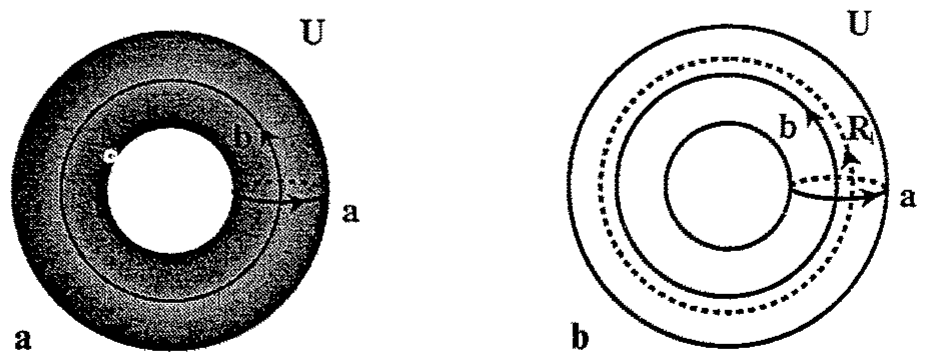
\includegraphics[width=0.64\linewidth]{figures/fig13.png}
    \caption{a 中亏格一的黎曼面 $\Sigma$ 被画成实心环面 $U$ 的边界；图中标出的 $a$ 圈在 $U$ 中可缩。b 中给出物理希尔伯特空间的一组基：在 $U$ 内部沿与 $b$ 圈平行的方向放置处于 $R_i$ 表示的威尔逊线，作路径积分即得 $\mathcal{H}_\Sigma$ 中的向量 $v_i$。（原文 p.~384，Fig.~13）}
\end{figure}

$v_i$ 构成 $\mathcal{H}_\Sigma$ 中的 Verlinde 基。必须明白：处于平凡表示的威尔逊线
等于 1，因此由上述定义得到的向量 $v_0$，与上一小节中在 $U$ 上不作任何威尔逊线插入、
仅由路径积分得到的向量 $\chi$ 相同：

\begin{equation}
    \chi = v_0 . \tag{4.24}
\end{equation}

$\Sigma$ 的一个微分同胚 $K$ 在 Verlinde 基下由一个显式的矩阵 $K_i{}^j$ 表示，
其定义为

\begin{equation}
    K\cdot v_i = \sum_j K_i{}^j v_j . \tag{4.25}
\end{equation}

% [Tutor Note: $S$ 矩阵与 $T$ 矩阵] 式 (4.25) 的 $K_i{}^j$ 就是环面微分同胚在特征标上的
% 表示；而 $\mathrm{SL}(2,\mathbb{Z})$ 由 $S:\tau\mapsto-1/\tau$ 与 $T:\tau\mapsto\tau+1$
% 生成，所以只需知道两个矩阵即可。$T$ 是对角的：
% $T_i{}^j=\delta_i^j\exp\bigl(2\pi i(h_i-c/24)\bigr)$，其中 $h_i$ 是第 $i$ 个初级场的
% 共形权，$c$ 是中心荷（$\mathrm{SU}(N)_k$ 时 $c=k(N^2-1)/(k+N)$）；$S_i{}^j$ 是 Verlinde
% 的融合矩阵，其第一列（或第一行）$S_{0i}$ 给出量子维数。二者满足
% $(ST)^3=S^2=C$、$C^2=1$（$C$ 为电荷共轭矩阵），这正是 $\mathrm{SL}(2,\mathbb{Z})$
% 的投影表示；$S$ 在适当归一化下对称且幺正。注意 $T$ 中的 $c/24$ 相位是一个整体相位，
% 它不影响 $|Z|$，却改变配分函数的标架依赖——这与 p.382 附近 (4.20) 之前那处标架修正同源，
% 比较文献时极易漏掉。

在 $v_i$ 张成的空间上有一个自然的内积，它由张量 $g_{ij}$ 定义：若 $R_i$ 是 $R_j$ 的对偶，
则 $g_{ij}$ 等于 1，否则为零。我们有时会用这个度规来升降指标，即令
$K_{ij}=\sum_m g_{mj}K_i{}^m$。

% [Tutor Note: 指标位置易错] (4.25)–(4.28) 的指标约定很容易写错。$K_i{}^j$ 是线性变换的
% 矩阵，$i$ 是源指标（写在下方）、$j$ 是像指标（写在上方）；$v_0$ 对应平凡表示 $R_0$，
% 所以 (4.26) 中出现的是 $K_0{}^j$（第 0 行的元素），而不是 $K_j{}^0$。又因 $g_{ij}$ 只在
% $R_i$ 与 $R_j$ 互为对偶时才为 1（它不是 $\delta_{ij}$），
% $K_{ij}=\sum_m g_{mj}K_i{}^m$ 是用 $g$ 把上指标降下来；若把 $g$ 的指标顺序写成 $g_{im}$，
% 得到的就会是 $K$ 的转置。另外 (4.28) 左边的表示标号 $R_i$ 与右边的求和指标 $j$
% 是两个不同的指标，不能同名缩并。做手术链环的具体计算时，这些下标直接决定最终多项式的
% 幂次，务必逐项核对。

现在我们可以更具体地描述该量子场论配分函数在手术下的行为。讨论手术时，
我们从一个三维流形 $M$ 和一个纽结 $C$ 出发。挖去这个纽结的管状邻域，
其边界记作 $\Sigma$，就把 $M$ 分成了 $M_L$ 与 $M_R$，其中 $M_R$ 是实心环面。
$M_L$ 与 $M_R$ 上的路径积分给出希尔伯特空间 $\mathcal{H}_L$ 与 $\mathcal{H}_R$ 中的向量
$\psi$ 与 $\chi$。正如刚才指出的，$\chi$ 就是 $v_0$，所以 $M$ 上的配分函数是
$(\psi,v_0)$。现在要在 $M_R$ 的边界上作一个微分同胚 $K$，然后把 $M_L$ 与 $M_R$
粘在一起，得到新的三维流形 $\tilde{M}$。$\tilde{M}$ 的配分函数为
$Z(\tilde{M})=(\psi,Kv_0)$，这正如上一小节末尾所述。说 $Z(\tilde{M})$ 可由手术表示计算，
意思就是：$\tilde{M}$ 的这个不变量的计算可以化归为 $M$ 上可处理的计算。
下面我们来说明这一点。由式 (4.25) 可以写出

\begin{equation}
    Z(\tilde{M}) = \sum_j K_0{}^j\,(\psi,v_j). \tag{4.26}
\end{equation}

但每一项 $(\psi,v_j)$ 在 $M$ 上的路径积分中都有解释！事实上，$v_j$ 的定义恰恰是：
$v_j$ 与 $v_0$ 只相差在 $M_R$ 的中心插入一条处于 $R_j$ 表示的额外威尔逊线。
所以，正如 $(\psi,v_0)$ 代表 $M$ 的原始配分函数，$(\psi,v_j)$ 代表在 $C$ 上放置一条
处于 $R_j$ 表示的额外威尔逊线之后修改过的配分函数。于是把 (4.26) 改写成

\begin{equation}
    Z(\tilde{M}) = \sum_j K_0{}^j\cdot Z(M;R_j), \tag{4.27}
\end{equation}

其中 $Z(M;R_j)$ 是 $M$ 的配分函数，它在圆周 $C$ 上额外地包含一条处于 $R_j$ 表示的
威尔逊线（此外还有 $M$ 上原本已经存在的那些威尔逊线）。这一点在图 12c 中作了图示。
要使用 (4.27)，需要知道矩阵 $K_i{}^j$；它恰好是环面的微分同胚 $K$ 在圈群 $LG$
的能级 $k$ 不可约表示的特征标（character）上所表示的矩阵。这些矩阵出现在 [37] 中，
并且具有若干引人注目的性质，最近在 [12,13] 中得到了研究。已知 $K_i{}^j$ 之后，
(4.27) 就是一个完全显式的公式，它把 $\tilde{M}$ 上的计算表示成 $M$ 上的计算。
反复使用这个公式，任何三维流形上的计算都可以化归为 $S^3$ 上的计算，%
\footnote{或者在任意指定的三维流形上；我们将看到 $S^2\times S^1$ 比 $S^3$ 更容易处理。}
只需配上适当的威尔逊线。当然，手术会在 $S^3$ 上产生威尔逊线，
它们处于 $G$ 的各种表示之中，而这些表示对应于 $LG$ 的任意可积表示。

\textbf{广义手术（Generalized Surgery）。}手术律 (4.27) 有一个有用的推广。到目前为止，我们只考虑了在一条纯粹虚构的
（purely imaginary）圆周 $C$ 上作手术的情形，如图 12 所示；其实没有理由不把它推广到
如下情形：在手术之前，$C$ 上已经存在一条处于 $R_i$ 表示的威尔逊线。手术就是把 $C$
的邻域挖去、再把它粘回来；经过这一过程之后，这条 $R_i$ 威尔逊线仍然留在
$\tilde{M}$ 中。于是 (4.27) 的左边被替换为 $Z(\tilde{M};R_i)$，
这个记号示意性地表示 $R_i$ 威尔逊线的存在。那么 (4.27) 的右边呢？手术之前，
$C$ 上有一条 $R_i$ 威尔逊线，$C$ 的管状邻域 $U$ 上的路径积分在边界上给出一个态
$\chi'=v_i$；这是 (4.24) 的推广。如果挖去 $C$、再用边界的微分同胚 $K$ 把它粘回，
那么按 (4.25)，$v_i$ 被替换为 $K_i{}^j v_j$。如果我们记得 $v_j$ 可以通过在 $C$ 上
放置处于 $R_j$ 表示的威尔逊线得到，就会看到 (4.27) 的右边变成
$\sum_j K_i{}^j Z(M;R_j)$，于是得到广义手术公式

\begin{equation}
    Z(\tilde{M};R_i) = \sum_j K_i{}^j Z(M;R_j). \tag{4.28}
\end{equation}

这个公式稍后将在 Verlinde 猜想的一个新证明中用到。

\textbf{纽结的缆化；卫星（Cabling of Knots; Satellites）。}最后指出，类似的方法可以用来确定纽结不变量在“缆化”（cabling）下的行为，
更一般地，可以把一个纽结的“卫星”（satellite）的不变量与原来纽结的不变量联系起来。
任意三维流形 $M$ 中的任意纽结 $C$ 都有一个看起来像实心环面 $U$ 的邻域。
如果把 $C$ 换成它自己的任意一个卫星 $\hat{C}$（即一个能够放进 $U$ 中的任意纽结），
并为 $\hat{C}$ 的各个连通分支配上表示 $R_\sigma$，那么 $U$ 上的路径积分将在与 $U$
的边界 $\Sigma$ 相联系的物理希尔伯特空间 $\mathcal{H}_\Sigma$ 中定义一个向量 $\psi$。
与 $\mathcal{H}_\Sigma$ 中任何向量一样，$\psi$ 可以在 Verlinde 基中展开：

\begin{equation}
    \psi = \sum_i \alpha_i v_i . \tag{4.29}
\end{equation}

这些 $\alpha_i$ 是复数，它们依赖于卫星 $\hat{C}$ 的选取以及表示 $R_\sigma$ 的选取，
但不依赖于实心环面 $U$ 是从哪个三维流形 $M$ 中取出的，也不依赖于 $M$ 上还存在着
哪些其他纽结。向量 $v_i\in\mathcal{H}_\Sigma$ 则是在原来纽结 $C$ 上（而不是在 $C$
的某个卫星上）放置处于 $R_i$ 表示的威尔逊线后、由 $U$ 上的路径积分得到的向量。
因此，只要知道 $C$ 在任意表示下的不变量，再加上这些普适系数 $\alpha_i$，
就足以确定 $C$ 的任意卫星的不变量。

\subsection{\texorpdfstring{$S^1\times X$ 上的路径积分}{S1×X 上的路径积分}}
% （本节重点见 §4 开头片段）

\begin{figure}[htbp]
    \centering
    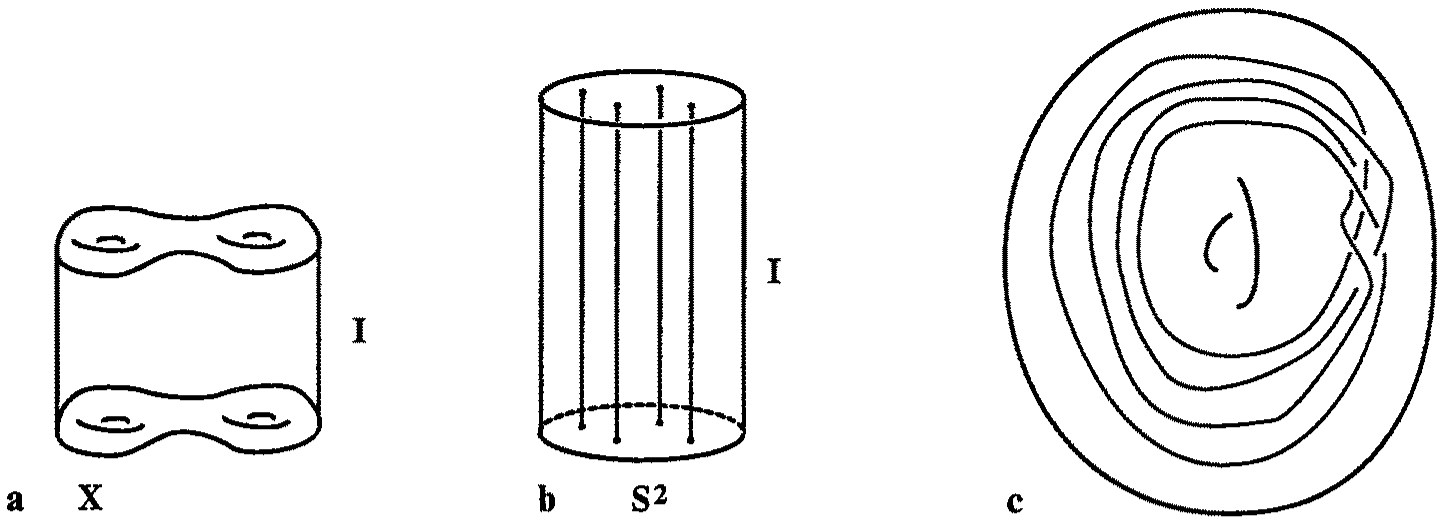
\includegraphics[width=1.00\linewidth]{figures/fig14.png}
    \caption{从 a 中的 $X\times I$ 出发，把 $X\times\{0\}$ 与 $X\times\{1\}$ 认同，即得 $X\times S^1$。若 $X$ 是带有若干标记点 $P_i$ 的 $S^2$，则该构造给出 b 中的图。若 $S^2\times\{0\}$ 与 $S^2\times\{1\}$ 之间通过非平凡的微分同胚 $B$ 粘合，就得到 c 中的辫。图注中的微分同胚 $B$ 即正文 (4.32) 之 $K$。（原文 p.~387，Fig.~14）}
\end{figure}

本小节将叙述几个本身就有用的事实，它们使我们能够进行一些具体的手术计算。

首先，我们迄今还没有确定不带威尔逊线的 $S^3$ 的配分函数。对拓扑学家来说，
也许令人惊讶的是：我们不能简单地断言它就等于 1。在量子场论中，并没有哪条特别强的
公理规定 $S^3$ 的配分函数应当为何。按量子场论的公理，其配分函数可以特别简单地计算
出来的三维流形，是形如 $X\times S^1$ 的那些流形（$X$ 各异）。$X\times S^1$ 可以方便地
用“哈密顿”形式来研究，如图 14a 所示。先构造 $X$ 的希尔伯特空间 $\mathcal{H}_X$。
然后引入一个“时间”方向，用单位区间 $I=[0,1]$ 表示，并把 $\mathcal{H}_X$ 中的向量从
“时刻” 0 演化到“时刻” 1。这一操作是平凡的，因为陈–西蒙斯理论像任何广义协变理论一样，
哈密顿量为零。最后，把 $X\times\{0\}$ 与 $X\times\{1\}$ 粘起来得到 $X\times S^1$；
这就把初态与末态等同起来，从而给出一个迹：

\begin{equation}
    Z(X\times S^1) = \mathrm{Tr}_{\mathcal{H}_X}(1) = \dim\mathcal{H}_X . \tag{4.30}
\end{equation}

% [Tutor Note: $S^1\times X$、绕数为零的模空间与拓扑不变量] 式 (4.30) 把
% $S^1\times X$ 的配分函数化成希尔伯特空间的维数，依据是“路径积分＝态的迹”这一标准论证：
% 陈–西蒙斯理论的哈密顿量为零（广义协变），沿 $S^1$ 的演化算符就是恒等算符，
% 把初末态等同后便得到 $\mathrm{Tr}(1)$。若想在路径积分一侧理解，可先在半经典
% （$k\to\infty$）图像下把积分局域化到平坦联络：$S^1\times X$ 上的平坦 $G$-联络由
% $\pi_1(S^1\times X)=\mathbb{Z}\times\pi_1(X)$ 到 $G$ 的同态（模共轭）给出，
% 沿 $S^1$ 的和乐作为一个扇区标签（绕数扇区）。绕数为零、即沿 $S^1$ 的和乐平凡的扇区里，
% 问题退回 $X$ 上平坦联络的模空间 $\mathcal{M}_{\mathrm{flat}}(X)$，其几何量子化正是
% $\mathcal{H}_X$（Verlinde）。因此 (4.30) 可以读作“对所有绕数扇区求和”的量子化结果：
% 对 $X=S^2$，$\pi_1(S^2)=1$，$\mathcal{M}_{\mathrm{flat}}(S^2)$ 是单点，
% $\dim\mathcal{H}_{S^2}=1$，于是得到 (4.31) 的 $Z(S^2\times S^1)=1$；对 $X=T^2$，
% (4.30) 给出 $\dim\mathcal{H}_{T^2}=t$，与 §4.3 的 Verlinde 结果一致。提醒读者：
% 不要把 (4.30) 误读成“$Z$ 恒等于 1”——它只对 $X\times S^1$ 这种特殊拓扑成立；
% 不带威尔逊线的 $S^3$ 的 $Z$ 并不由公理给出（见本小节开头），要到后面用手术才能定出。

例如，$S^2$ 的物理希尔伯特空间对任意 $G$ 和 $k$ 都是一维的，因此有

\begin{equation}
    Z(S^2\times S^1) = 1 . \tag{4.31}
\end{equation}

式 (4.30) 可以如下推广。若给定一个微分同胚 $K:X\to X$，就可以通过把
$x\times\{1\}$ 与 $K(x)\times\{0\}$ 对每个 $x\in X$ 等同起来，构造出映射柱面
（mapping cylinder）$X\times_K S^1$。在量子场论层面，当从 $X\times I$ 过渡到
$X\times_K S^1$ 时，初态与末态通过 $K$ 等同，因此 (4.30) 的推广是

\begin{equation}
    Z(X\times_K S^1) = \mathrm{Tr}_{\mathcal{H}_X}(K) . \tag{4.32}
\end{equation}

我们真正要应用这一结果的情形是：$X$ 是带有若干标记点 $P_a$（$a=1\dots s$）的 $S^2$，
而这些标记点上赋有表示 $R_{i(a)}$。


% =============================================================================
%  §4.5  一些具体的手术（Some Concrete Surgeries）
%  覆盖：PDF p.38 顶部（§4.4 收尾，承 p.37 末句）— p.43 末；印刷 pp.388–393
%  编号公式：(4.33)–(4.54)，逐号对应原文，无跳号
%  插图标记：FIG:15（p.38 首次提及，图见 p.39）、FIG:16（p.38 首次提及）、
%            FIG:17（p.41 末首次提及，图见 p.42）
% =============================================================================
% （4.4 节收尾，承 p.37）

[对 $a=1,\dots,s$，$i(a)$ 取 $0,\dots,t-1$ 中的某个值，它对应圈群的能级 $k$ 可积表示。] 在这种情形下，简单乘积 $X\times S^1$ 就是 $S^2\times S^1$ 再带上若干威尔逊线；这些威尔逊线不打结，是形如 $\{P_a\}\times S^1$ 的平行圆圈，如图 14b 所示。要确定在存在这些威尔逊线时 $S^2\times S^1$ 上的路径积分——我们把它记作 $Z(S^2\times S^1;\langle R\rangle)$——就需要研究 $S^2$ 上带处于表示 $R_{a_i}$ 中的电荷的希尔伯特空间；我们把它记作 $\mathcal{H}_{S^2;\langle R\rangle}$。式 (4.31) 的类比便是
% [Tutor Note: 此处 $R_{a_i}$ 与 p.387 末尾所写的 $R_{i(a)}$ 是同一对象（原文两页记号不一致，本译照印本 p.388 的写法）。$\mathcal{H}_{S^2;\langle R\rangle}$ 即带 $s$ 个插入点的黎曼球（球面）上的共形块空间：$S^2$ 作为空间切片，穿过标记点的威尔逊线给出电荷；Gauss 定律要求总荷为单态，所以单电荷只有在表示平凡时才可能有无穷小态，这正是 (4.34) 的来源。]
\begin{equation}
    Z(S^2\times S^1;\langle R\rangle) = \dim \mathcal{H}_{S^2;\langle R\rangle}. \tag{4.33}
\end{equation}
这些空间的维数已在第 3 节末尾讨论过。于是，若表示族 $\langle R\rangle$ 只含一个表示 $R_a$，就得到
\begin{equation}
    Z(S^2\times S^1;R_a) = \delta_{a,0}, \tag{4.34}
\end{equation}
因为单个处于 $R_a$ 表示的电荷所对应的物理希尔伯特空间，在 $R_a$ 为平凡表示（$a=0$）时是一维的，否则为零维。\footnote{式 (4.34) 及其后各式隐含了威尔逊线采用标准标架这一选择；该标架在 $S^1$ 的旋转下不变。正是对这一选择，$S^2\times S^1$ 上的路径积分才给出物理希尔伯特空间中恒等算符的迹。} 对分别处于 $R_a$、$R_b$ 表示的两个电荷，得到
\begin{equation}
    Z(S^2\times S^1;R_a,R_b) = g_{ab}, \tag{4.35}
\end{equation}
其中 $g_{ab}$ 是前面引入的量：当 $R_b$ 是 $R_a$ 的对偶表示时取 $1$，否则取 $0$。式 (4.35) 可由第 4.4 节关于 $S^2$ 上带两个电荷的希尔伯特空间的结果得到。最后，若有三个电荷，分别处于 $R_a$、$R_b$、$R_c$ 表示，则得到
\begin{equation}
    Z(S^2\times S^1;R_a,R_b,R_c) = N_{abc}, \tag{4.36}
\end{equation}
其中 $N_{abc}$ 是 Verlinde 的三线性“耦合”，因为它是物理希尔伯特空间的维数。
% [Tutor Note: (4.33)–(4.36) 把 $S^2\times S^1$ 上的路径积分归结为 $S^2$ 上物理希尔伯特空间的维数，这是 (4.30)（$Z(X\times S^1)=\dim\mathcal{H}_X$）的直接应用。注意维数序列：1 个电荷给出 $\delta_{a,0}$；2 个电荷给出 $g_{ab}$（对偶度规）；3 个电荷给出 $N_{abc}$（融合系数）。(4.36) 正是 Verlinde 公式中融合系数的路径积分定义；后文 (4.46)、(4.51) 都要回到它。]

\subsection{一些具体的手术}
% （本节重点见 §4 开头片段）
% [Tutor Note: 原文 "The first goal is compute the partition function of $S^3$" 脱一 "to"，应为 "is to compute"（本译按语义译出）；同页 "the result of Sect. (4.4)" 的编号写法也可疑，上下文指向的是 §4.4 末尾（或 §3.4），不损文义，但引用时宜写作 §4.4。]

现在我们要介绍一些可由具体手术得到的有用结果。第一个目标是计算 $S^3$ 的配分函数。既然已经知道 $S^2\times S^1$ 的配分函数，我们就试着把 $S^3$ 解释为在 $S^2\times S^1$ 上做手术所得的流形。这很容易做到。考虑 $S^2\times S^1$ 中如图 15a 所示的圆圈 $C$。$C$ 的管状邻域是一个环面 $\Sigma$；我们取 $H^1(\Sigma;\mathbb{Z})$ 的一组基，由图中标出的循环 $a$ 与 $b$ 组成。

\begin{figure}[htbp]
    \centering
    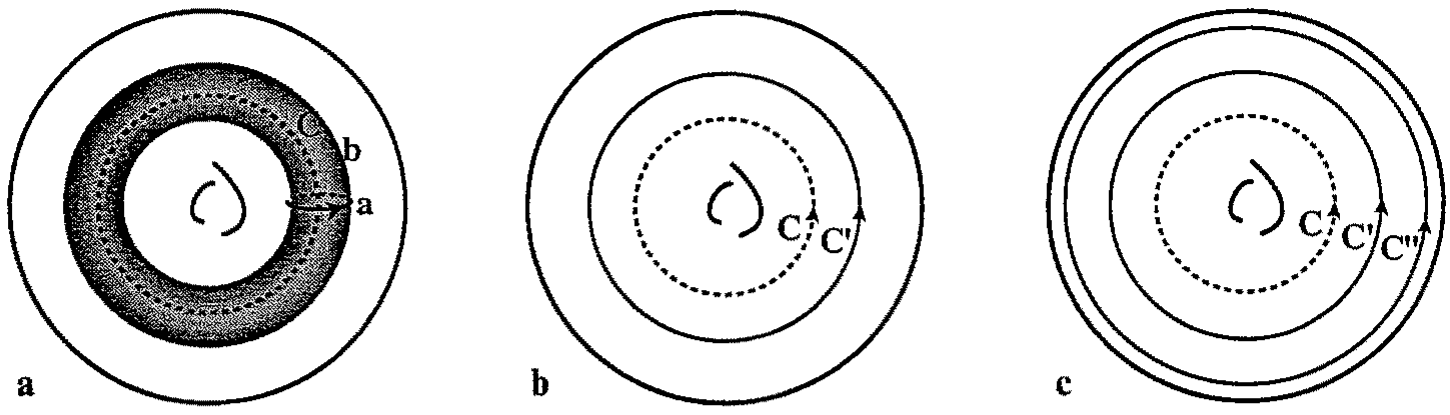
\includegraphics[width=1.00\linewidth]{figures/fig15.png}
    \caption{a 中考虑对 $S^2\times S^1$ 中的圆圈 $C$ 做手术，其管状邻域是一个环面 $\Sigma$，图中标出 $H^1(\Sigma,\mathbb{Z})$ 的一组有用的基。b 中除手术所沿的圆圈 $C$ 外，还有一条与它平行的圆圈 $C'$，其上放置处于 $R_j$ 表示的威尔逊线。c 中有两条平行圆圈 $C'$ 与 $C''$，其上分别放置处于 $R_j$ 与 $R_k$ 表示的威尔逊线。（原文 p.~389，Fig.~15）}
\end{figure}

% [Tutor Note: 图 15 三部分的含义先交代清楚（后文 p.391 才用到 b、c）：a 中画出 $S^2\times S^1$ 中做手术的圆圈 $C$ 及其管状邻域边界环面 $\Sigma$ 上的基 $a,b$；b 中在 $C$ 旁边平行地加一条圆圈 $C'$，其上放 $R_j$ 表示的威尔逊线；c 中放两条平行圆圈 $C',C''$，带 $R_j$、$R_k$ 表示。这些威尔逊线都取标准标架（沿 $S^1$ 旋转不变的标架，见 (4.34) 后脚注），因此手术后在 $S^3$ 上得到标准标架下的不打结威尔逊线，这是后面能用纯 $S$ 矩阵表示配分函数的原因。]

现在我们要做一次特殊的手术，它联系着一个非常特殊的微分同胚 $S\colon\Sigma\to\Sigma$。取 $S$ 把 $a$ 映到 $b$，把 $b$ 映到 $-a$。\footnote{这一变换在上半平面上的作用为 $\tau\to-1/\tau$，在模群 $\mathrm{SL}(2,\mathbb{Z})$ 的理论中确实通常称为 $S$（借助基 $a$、$b$，$\mathrm{SL}(2,\mathbb{Z})$ 可与 $\Sigma$ 的映射类群等同）。} 这项手术——把以 $\Sigma$ 为边界的实心环内部从 $S^2\times S^1$ 中挖去，再经 $S$ 作用后粘回去——所产生的三维流形不是别的，正是 $S^3$（图 16）。
% [Tutor Note: 这里的微分同胚 $S$ 与后文的“$S$ 矩阵”是同一个对象。在基 $a,b$ 下它的矩阵是 $\begin{pmatrix}0&-1\\1&0\end{pmatrix}$，正是模变换 $\tau\mapsto-1/\tau$ 的表示（差一个整体符号；在 $PSL(2,\mathbb{Z})$ 中 $S^2=1$）。这正是本节全套机制的来源：沿 $C$ 以粘合映射 $S$ 做手术恰好把 $S^2\times S^1$ 变成 $S^3$，而手术公式 (4.27) 的系数正是 $S$ 矩阵元 $S_0{}^j$。极易出错之处：粘合映射的选取与 $a,b$ 的定向一旦改变，$S$ 会换成 $S^{-1}$、$T$ 会换成 $T^{-1}$——这对 (4.38) 的数值无关紧要，却会改变 (4.41) 的相位，务必逐项核对。]

\begin{figure}[htbp]
    \centering
    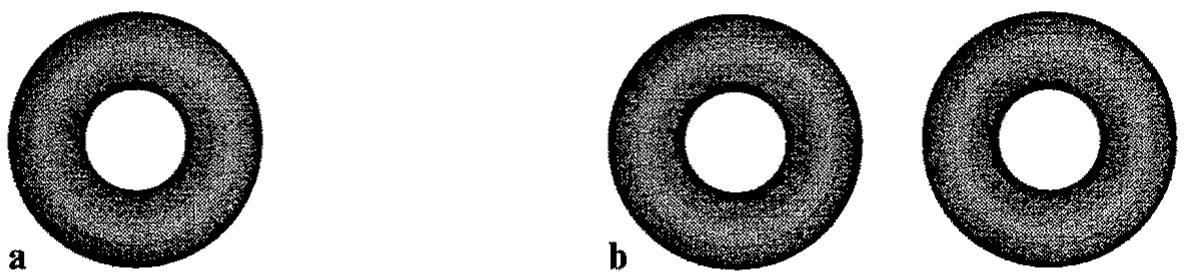
\includegraphics[width=0.82\linewidth]{figures/fig16.png}
    \caption{本图旨在说明如何从 $S^2\times S^1$ 出发、通过手术得到 $S^3$。a 画出位于 $\mathbb{R}^3$ 中的环面 $\Sigma$；b 画出一对全同的实心环面。（原文 p.~389，Fig.~16）}
\end{figure}

由于这一点在后续讨论中至关重要，我们暂停一下来加以说明。把 $S^3$ 看作 $\mathbb{R}^3$ 加上一个无穷远点。图 16a 把一个环面 $\Sigma$ 嵌入到 $\mathbb{R}^3$ 中。显然，$\Sigma$ 连同它的内部构成一个实心环 $T$。也不难看出，图 (a) 在反演下不变，因此 $\Sigma$ 的外部（包括无穷远点）也是另一个实心环 $T'$。于是，$S^3$ 可以由两个实心环沿其边界粘合而成。接下来，在 (b) 中我们画出两个相同的实心环 $T$ 与 $T'$；$T'$ 由 $T$ 在欧氏空间中简单平移得到。若把两者的边界逐点粘合——所谓“$T'$ 是 $T$ 的平移”所指的正是这种等同——得到的就是 $S^2\times S^1$。（事实上，实心环 $T$ 是 $D\times S^1$，$D$ 是一个二维圆盘；$T'$ 是 $D'\times S^1$，$D'$ 是第二个圆盘。正如两个圆盘 $D$、$D'$ 沿边界粘合得到 $S^2$，$D\times S^1$ 与 $D'\times S^1$ 自然粘成 $S^2\times S^1$。）另一方面，由 (a) 可知 $S^3$ 也能由两个实心环粘合得到。稍加思维演练，把 (a) 处的论证与 (b) 处的论证作一比较，就会看出：要得到 $S^3$，必须先在 $T'$ 的边界上作模变换 $S$，再把 $T$ 与 $T'$ 粘合起来。
% [Tutor Note: “图 (a) 在反演下不变”是本节被略过的一步，其核心逻辑是：在 $S^3=\mathbb{R}^3\cup\{\infty\}$ 中取绕某圆周的标准环面 $\Sigma$，反演 $x\mapsto x/|x|^2$ 是共形微分同胚，它把 $\Sigma$ 映到自身并把内部与外部互换；故 $\Sigma$ 外部连同无穷远点的闭包也是实心环 $T'$。这就是 $S^3$ 的亏格 1 Heegaard 分解 $S^3=T\cup_{\partial}T'$。图 16b 按“平移”粘合两个实心环得 $S^2\times S^1$，而按模变换 $S$ 粘合得 $S^3$——两者只差边界粘合映射，这正是 (4.37) 的系数为 $S_0{}^j$ 的几何根源。]

现在可以使用式 (4.27)：让 $S^3$ 扮演 $\tilde{M}$ 的角色，$S^2\times S^1$ 扮演 $M$ 的角色，而任意的微分同胚 $K$ 换成 $S$。于是得到
\begin{equation}
    Z(S^3) = \sum_j S_0{}^j\, Z(S^2\times S^1;R_j). \tag{4.37}
\end{equation}
由上一小节已知，$Z(S^2\times S^1;R_j)$ 当 $j=0$ 时为 $1$、否则为 $0$，所以
\begin{equation}
    Z(S^3) = S_{0,0}. \tag{4.38}
\end{equation}
% [Tutor Note: $S_{0,0}$ 的物理意义是“总量子维数的倒数”：对一般的有理共形场论，$Z(S^3)=S_{0,0}=1/D$，其中 $D^2=\sum_j d_j^2$，而 $d_j=S_{0,j}/S_{0,0}$ 是表示 $R_j$ 的量子维数。对 $SU(2)$，由 (4.39) 取 $m=n=0$ 得 $S_{0,0}=\sqrt{2/(k+2)}\,\sin(\pi/(k+2))$，正是 (2.26) 中已有的公式。注意配分函数的绝对归一化不是可以任意设定的——§4 开头已论证 $Z(S^3)$ 被场论公理唯一确定，(4.38) 就是它的具体取值，后文 (4.43) 中 $Z(S^3;R_j)=S_{0,j}$ 与它相比才给出量子维数。]

这里 $S_{0,0}$ 可由仿射李代数理论确定；对 $G=\mathrm{SU}(2)$，得到前面 (2.26) 中已写出的公式。事实上，对 $G=\mathrm{SU}(2)$，整个矩阵 $S_{ij}$ 都可以写得很显式。能级 $k$ 的可积表示就是自旋为 $n/2$ 的表示，$n=0,\dots,k$，而 $S$ 的矩阵元为
\begin{equation}
    S_{mn} = \sqrt{\frac{2}{k+2}}\;\sin\frac{(m+1)(n+1)\pi}{k+2}. \tag{4.39}
\end{equation}
% [Tutor Note: (4.39) 给出的 $S$ 矩阵是幺正的、对称的：$S_{mn}=S_{nm}$，$\sum_n S_{mn}S_{m'n}=\delta_{mm'}$；指标 $n=0,\dots,k$ 对应自旋 $n/2$。由 (4.39) 得 $S_{0,n}=\sqrt{2/(k+2)}\,\sin((n+1)\pi/(k+2))$，而比值 $S_{0,n}/S_{0,0}=\sin((n+1)\pi/(k+2))/\sin(\pi/(k+2))$ 就是自旋 $n/2$ 的量子维数——这正是 (4.44) 分子的来源。另外注意原文此处写 $S_{mn}$（无逗号），而本节别处写 $S_{0,j}$（有逗号），只是记号不统一，并非不同对象。]

\textbf{配分函数的相位（The Phase of the Partition Function）。} 现在用这些方法重新审视第 2 节出现的一个棘手问题——三维流形的标架，以及配分函数的相位。

我们是通过在某个圆圈 $C$ 上做手术、使用模变换 $S\colon\tau\to-1/\tau$，从 $S^2\times S^1$ 得到 $S^3$ 的。除 $S$ 之外，还可以用别的模变换在 $S^2\times S^1$ 中同一个纽结 $C$ 上做手术来构造 $S^3$。一般的选择是 $T^nST^m$，其中 $n$、$m$ 是任意整数，$T$ 是模变换 $T\colon\tau\to\tau+1$。［$S$ 与 $T$ 是模群的标准生成元，满足 $S^2=(ST)^3=1$。］若用 $T^nST^m$，得到的将不是 (4.38)，而是
\begin{equation}
    Z(S^3) = (T^nST^m)_{0,0}. \tag{4.40}
\end{equation}
这很容易算出。在 Verlinde 基中，$T$ 是对角矩阵，$T\cdot v_i=e^{2\pi i(h_i-c/24)}\cdot v_i$；$h_i$ 是表示 $R_i$ 中初级场的共形权，$c$ 是对称群为 $G$、能级为 $k$ 的流代数的中心荷。由于 $h_0=0$，若把 (4.38) 换成 (4.40)，配分函数就按
\begin{equation}
    Z \to Z\cdot\exp\left(2\pi i(n-m)\cdot\frac{c}{24}\right) \tag{4.41}
\end{equation}
变换。
% [Tutor Note: (4.40)–(4.41) 是本文第一次定量讨论“标架反常”，极易出符号错误。核对办法：由 (2.24) 的大 $k$ 极限可知标架歧义给出 $e^{\pm2\pi i c/24}$ 型相位。(4.41) 中 $n$ 与 $m$ 的符号相反（$e^{2\pi i(n-m)c/24}$）不是笔误，它对应后文的一般规则——“把 $u$ 换成 $uT^m$ 会多出相位 $e^{-2\pi im\,c/24}$”；换言之，左侧 $T^n$ 贡献 $e^{+2\pi in\,c/24}$，右侧 $T^m$ 贡献 $e^{-2\pi im\,c/24}$。若要推广到任意手术，必须把三维流形换成“带标架的”三维流形，这就是 Witten 说“将在别处系统讨论”的内容（标架反常／2+1 维拓扑场论的标架依赖）。]

虽然这一公式是在一个特定手术（由 $S^2\times S^1$ 得到 $S^3$）的例子中得到的，但同样的歧义出现在任何手术过程中。只要在三维流形 $M$ 中沿圆圈 $C$ 做手术，且手术由 $\mathrm{SL}(2,\mathbb{Z})$ 元素 $u$ 决定，就可以改为沿同一圆圈 $C$、用 $\mathrm{SL}(2,\mathbb{Z})$ 元素 $u\cdot T^m$ 做手术。这在拓扑上效果相同，但按我们的手术法则，配分函数会多出一个相位 $\exp(-2\pi im\cdot c/24)$。

这个相位歧义在大 $k$ 极限下已在公式 (2.24) 中遇到过。而且，由第 2 节的讨论我们知道，要追踪 $\exp(2\pi i\cdot c/24)$ 的因子，必须在三维流形上考虑什么样的拓扑结构。必须考虑“带标架的”三维流形。两个对三维流形拓扑有相同效果的手术，对标架的效果可能不同。我将在别处讨论如何在手术下系统地追踪 $\exp(2\pi i\cdot c/24)$ 的因子。在本文的简单应用中，这没有必要。我们的全部应用都只涉及上一小节用来从 $S^2\times S^1$ 得到 $S^3$ 的标准手术（用模变换 $S$）。

\textbf{一些期望值（Some Expectation Values）。} 现在看看能否再进一步，确定 $S^3$ 上带一条不打结威尔逊线（位于任意表示 $R_j$ 中）的路径积分 $Z(S^3;R_j)$。\footnote{我们让这条威尔逊线采用 (4.34) 后脚注所述的标架；手术后它就成为 $S^3$ 上的标准标架。} 为此，我们从 $S^2\times S^1$ 出发，在其上放一条处于 $R_j$ 表示、与将要做手术的圆圈 $C$ 平行的威尔逊线，如图 15b 所示。施行与前面相同的手术，就把 $S^2\times S^1$ 变成 $S^3$，同时在 $S^3$ 上留下一条 $R_j$ 表示的威尔逊线。应用 (4.27) 得到
\begin{equation}
    Z(S^3;R_j) = \sum_i S_0{}^i\, Z(S^2\times S^1;R_i,R_j). \tag{4.42}
\end{equation}
利用 (4.35)，可以算出它，从而确定任意表示 $R_j$ 中威尔逊线的配分函数：
\begin{equation}
    Z(S^3;R_j) = \sum_i S_0{}^i g_{ij} = S_{0,j}. \tag{4.43}
\end{equation}
% [Tutor Note: 指标位置在此极易混淆：Witten 把 $S$ 矩阵元写成 $S_{0,j}$（下标、带逗号），又写成 $S_0{}^j$ 或 $S_0{}^i$（下标 $0$、上标 $j$ 或 $i$），二者数值相同只因 $S$ 对称、并用 $g_{ij}$ 升降指标。切勿把 $S_0{}^i g_{ij}$ 误读为普通的矩阵乘法之外的东西：$g_{ij}$ 是电荷共轭度规（对 $SU(2)$ 为 $g_{ij}=\delta_{i\bar j}$），它把 $R_i$ 的对偶指标降下来，所以 (4.43) 的求和把 $S_0{}^i$ 变成 $S_{0,j}$；同理 (4.47) 第二步中 $\sum_k S_i{}^k g_{kj}=S_{ij}$。]

让我们把它与先前对 $S^3$ 中不打结威尔逊线期望值的计算 (4.23) 作比较。必须记得，(4.23) 中的符号 $\langle C\rangle$ 代表一个比值 $\langle C\rangle=Z(S^3;R)/Z(S^3)$。取 $G=\mathrm{SU}(2)$，以便使用显式公式 (4.39)；并取 $R$ 为 $\mathrm{SU}(2)$ 的二维表示，以便与 (4.23) 比较。利用 (4.38)、(4.43)、(4.39)，得到
\begin{equation}
    \langle C\rangle = \frac{S_{0,1}}{S_{0,0}} = \frac{\sin\,(2\pi/(k+2))}{\sin\,(\pi/(k+2))}. \tag{4.44}
\end{equation}
容易看出，在 (4.23) 中令 $N=2$ 就给出同一公式。
% [Tutor Note: 作者说“容易看出”，具体内容是：(4.23) 是 $SU(N)$ 能级 $k$、基本表示（$N$ 维）的公式 $\langle C\rangle=(q^{N/2}-q^{-N/2})/(q^{1/2}-q^{-1/2})$，其中 $q=\exp(2\pi i/(N+k))$（见 (4.21)）。取 $N=2$ 得 $q=e^{2\pi i/(k+2)}$，于是 $\langle C\rangle=q^{1/2}+q^{-1/2}=2\cos(\pi/(k+2))$；而 (4.44) 右端 $\sin(2\pi/(k+2))/\sin(\pi/(k+2))=2\cos(\pi/(k+2))$，两者一致。注意 (4.23) 中的 $N$ 同时是规范群 $SU(N)$ 的阶与基本表示的维数，取 $N=2$ 时这两重含义合而为一，最不易混淆。]

让我们再进一步，试着用这些方法计算 $S^3$ 上带两条不打结、不链接的威尔逊线（分别处于表示 $R_j$ 与 $R_k$）的配分函数 $Z(S^3;R_j,R_k)$。在图 15c 中，我们从 $S^2\times S^1$ 出发，其上放两条与待做手术的圆圈 $C$ 平行的威尔逊线，分别处于 $R_j$ 与 $R_k$ 表示。施行手术，就得到 $S^3$ 上所需的这两条不链接、不打结的圆圈。此时手术公式 (4.27) 告诉我们
\begin{equation}
    Z(S^3;R_j,R_k) = \sum_i S_0{}^i\, Z(S^2\times S^1;R_i,R_j,R_k). \tag{4.45}
\end{equation}
右端可用 (4.36) 计算，而左端可利用 (4.6) 归结为 (4.43)。于是得到
\begin{equation}
    \frac{S_{0,j}S_{0,k}}{S_{0,0}} = \sum_i S_0{}^i\, N_{ijk}. \tag{4.46}
\end{equation}
% [Tutor Note: (4.46) 左端来自 (4.6) 的乘性：$S^3$ 上两条不链接、不打结的威尔逊线的关联函数可分解为 $Z(S^3;R_j,R_k)=Z(S^3;R_j)Z(S^3;R_k)/Z(S^3)$（把图剪成两半，各自独立，再除以一个 $Z(S^3)$）；再用 (4.43)、(4.38) 即得 $S_{0,j}S_{0,k}/S_{0,0}$。这一分解显然对 $j,k$ 对称，与关联函数在交换两条威尔逊线下的对称性一致；右端则把 (4.36) 代入 (4.45)。(4.46) 就是 Verlinde 公式在三指标全对称情形的特例；(4.51) 只是把指标 $0$ 换成一般的 $i$，其证明（下段）正是本节的核心。]

\textbf{Verlinde 猜想的证明（Proof of Verlinde's Conjecture）。} 最后一个方程是 Verlinde 一个著名猜想的特例，该猜想已由 Moore 与 Seiberg [13] 证明。我们可以用这些方法在流代数的情形给出 Verlinde 猜想的一个新证明。我们将用到推广的手术关系 (4.28)。回到图 15b，但这次不把 $C$ 当作只做手术的纯虚轮廓，而假设 $C$ 上有一条处于 $R_i$ 表示的威尔逊线。此时沿 $C$ 的标准手术仍把 $S^2\times S^1$ 变成 $S^3$，但 $S^3$ 上将留下两条威尔逊线，分别处于 $R_i$ 与 $R_j$ 表示。稍加思维演练可知它们相互链接，如图 17a 所示；概要地说，我们把这成对的链接威尔逊线记作 $L(R_i;R_j)$。

\begin{figure}[htbp]
    \centering
    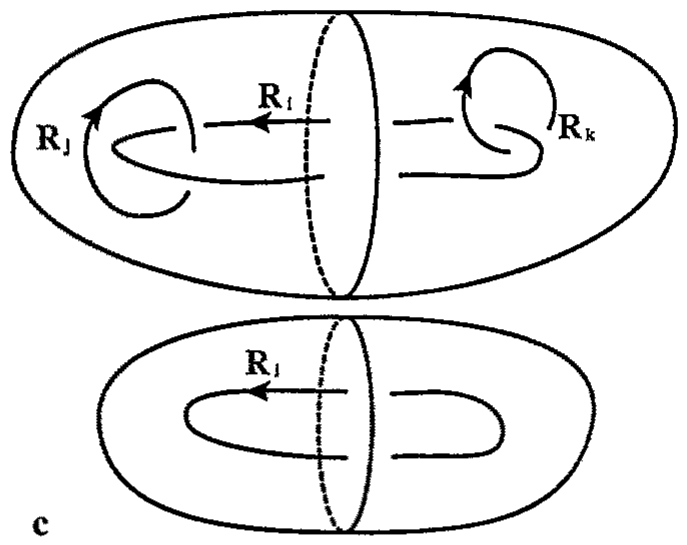
\includegraphics[width=0.47\linewidth]{figures/fig17.png}
    \caption{a 中画出 $S^3$ 上相互链接但各自平凡的威尔逊线，分别处于 $R_i$ 与 $R_j$ 表示。b 中一条 $R_i$ 威尔逊线与两条 $R_j$、$R_k$ 威尔逊线相链接。c 中示意两个关键振幅如何通过同一个一维空间分解。（原文 p.~392，Fig.~17）}
\end{figure}

于是 (4.28) 给出 $S^3$ 上带一对链接威尔逊线的配分函数：
\begin{equation}
    Z(S^3;L(R_i;R_j)) = \sum_k S_i{}^k\, Z(S^2\times S^1;R_k,R_j) = S_{ij}. \tag{4.47}
\end{equation}
第二步用到了这样的事实：$S^2\times S^1$ 上带静态电荷 $R_k$ 与 $R_j$ 的配分函数，就是我们称为 $g_{kj}$ 的度规——当 $R_k$ 是 $R_j$ 的对偶时取 $1$，否则取 $0$。
% [Tutor Note: (4.47)、(4.48) 用的是广义手术公式 (4.28)：原先只放“虚”手术圈 $C$ 的地方现在也带一条威尔逊线，于是手术后在 $S^3$ 上得到的不是平行威尔逊线，而是相互链接的威尔逊线。关键区别在于：平行威尔逊线的配分函数给 $g_{ij}$（对偶配对），链接威尔逊线的配分函数给 $S_{ij}$（$S$ 矩阵元）。请对照图 17a（$R_i$ 与 $R_j$ 相链）与图 17b（$R_i$ 同时与 $R_j$、$R_k$ 相链，而 $R_j$ 与 $R_k$ 彼此不链）来理解这两个公式的差别：这正是 Jones 多项式与 $S$ 矩阵之间的桥。]

现在回到图 15c，再次在原先那个纯虚圆圈 $C$ 上放一条处于 $R_i$ 表示的威尔逊线。对这一链环做标准手术，得到的图像如图 17b 所示：$S^3$ 上一条 $R_i$ 表示的威尔逊线与一对 $R_j$、$R_k$ 表示的威尔逊线相链接，而后者本身既不链接也不打结。我们把这个构型记作 $L(R_i;R_j,R_k)$。对 (4.28) 的计算现在给出
\begin{equation}
\begin{aligned}
    Z(S^3;L(R_i;R_j,R_k))
    &= \sum_m S_i{}^m\, Z(S^2\times S^1;R_m,R_j,R_k)\\
    &= \sum_m S_i{}^m\, N_{mjk}.
\end{aligned}
\tag{4.48}
\end{equation}
要得到 Verlinde 公式，现在需要找到独立计算左端的方法。
% [Tutor Note: 原文图注写的是 "Fig. 17a–c"（只有三部分），OCR 与一些二手材料常误作 a–e。逐步拆解如下：a 中 $R_i$ 与 $R_j$ 相链，来自图 15b 中平行的 $C'$ 与手术圈 $C$ 的链接；b 中 $R_i$ 同时与 $R_j$、$R_k$ 相链，而 $R_j,R_k$ 彼此不链，来自图 15c 的两条平行线；c 把 $L(R_i;R_j,R_k)$“剪开”，显示它是 $L(R_i;R_j)$ 与 $L(R_i;R_k)$ 的连通和——每一半都去掉一段连接线段，这正是链环连通和的定义性构型，(4.49) 的推理就是这一几何分解的代数化。]

这样的方法来自下面这个对乘性公式 (4.1) 的推广。推导 (4.1) 的关键在于：$S^2$ 上无电荷时的物理希尔伯特空间是一维的。同样，$S^2$ 上带一对分别处于对偶表示 $R_i$ 与 $R_{\bar i}$ 的电荷时，其物理希尔伯特空间 $\mathcal{H}$ 也是一维的。利用这一点，并照搬 (4.1) 的推导，便得到下面的公式：
\begin{equation}
\begin{gathered}
    Z(S^3;L(R_i;R_j,R_k))\cdot Z(S^3;R_i)\\
    = Z(S^3;L(R_i;R_j))\cdot Z(S^3;L(R_i;R_k)).
\end{gathered}
\tag{4.49}
\end{equation}
(4.49) 的想法是：如图 17c 所示，$Z(S^3;L(R_i;R_j,R_k))$ 的计算可以表示成一个配对 $(\psi,\chi)$，其中 $\psi$ 与 $\chi$ 是 $\mathcal{H}$ 及其对偶中的某些向量。同样，$Z(S^3;R_i)$ 的计算是一个配对 $(v',v)$，其中 $v'$ 与 $v$ 是 $\mathcal{H}$ 及其对偶中的向量。利用一维线性代数这一美妙事实 $(\psi,\chi)\cdot(v',v)=(\psi,v)\cdot(v',\chi)$，就得到 (4.49)。由于 (4.49) 中除第一项外各项都已知，我们得到
\begin{equation}
    Z(S^3;L(R_i;R_j,R_k)) = S_{ij}S_{ik}/S_{0,i}. \tag{4.50}
\end{equation}
% [Tutor Note: (4.49) 的“一维线性代数”可以这样理解：$\dim\mathcal{H}=1$ 时，任何配对 $\mathcal{H}\otimes\mathcal{H}^*\to\mathbb{C}$ 都是秩一的，于是两个配对的乘积满足 $(\psi,\chi)(v',v)=(\psi,v)(v',\chi)$——把 $\psi,\chi$ 与 $v',v$ 看成同一维空间及其对偶中的向量，交换收缩的次序不改变结果（等价于 $2\times2$ 行列式的秩一性）。图 17c 正是这个事实的几何版本：$L(R_i;R_j,R_k)$ 的振幅与 $Z(S^3;R_i)$ 都能通过同一个一维空间分解。]

把它与 (4.48) 结合，就有
\begin{equation}
    S_{ij}S_{ik}/S_{0,i} = \sum_m S_i{}^m\, N_{mjk}. \tag{4.51}
\end{equation}
这等价于 Verlinde 的命题“矩阵 $S$ 使融合规则对角化”。换言之，在图 13 所示的基 $v_i$ 中，Verlinde 代数的结构常数按定义为 $v_iv_j=\sum_k N_{ij}{}^k v_k$，其中 $N_{ij}{}^k=\sum_r N_{ijr}g^{rk}$。若引入新基 $w_i=S_{0,i}\cdot\sum_m S_i{}^m v_m$，则 Verlinde 代数化为 $w_iw_j=\delta_{ij}w_j$。为验证这一点，我们计算
\begin{equation}
    w_iw_j = \sum_{k,l} S_i{}^k S_j{}^l v_kv_l\cdot S_{0,i}S_{0,j}. \tag{4.52}
\end{equation}
利用 $v_kv_l=\sum_m N_{kl}{}^m v_m$ 与 (4.51)，上式变为
\begin{equation}
    w_iw_j = S_j{}^l v^m\cdot S_{il}S_i{}^m\cdot S_{0,j}. \tag{4.53}
\end{equation}
% [Tutor Note: (4.53) 是被略过的关键一步，且印本此处可疑：原文作 $v^m$（上标），但按 (4.52)→(4.54) 的逻辑应为 $v_m$（下标，对 $l,m$ 求和；本译照印本作 $v^m$，请以本注为准）。完整推导：把 (4.52) 中的 $v_kv_l$ 用 $v_kv_l=\sum_m N_{kl}{}^m v_m$ 展开后，先对 $k$ 用 (4.51) 的等价形式 $\sum_k S_i{}^k N_{kl}{}^m = S_{il}S_i{}^m/S_{0,i}$（此处用到 Verlinde 系数 $N$ 的全对称性以及 $g$ 升降指标），于是 (4.52) 中的 $S_{0,i}$ 恰好被约去，得 (4.53)；再用幺正性即得 (4.54)。这一“先用 (4.51) 消去 $S_{0,i}$”的步骤正是作者省略之处。]
利用 $S$ 的幺正性，写成 $S_j{}^l S_{il}=\delta_{ij}$，便看出
\begin{equation}
    w_iw_j = \delta_{ij}\sum_m S_j{}^m v_m\cdot S_{0,j} = \delta_{ij}\cdot w_j, \tag{4.54}
\end{equation}
这表明 Verlinde 代数已被对角化，且各 $w_i$ 是幂等元。

\textbf{链环的连通和（Connected Sum of Links）。} 第 4 节开头我们已看到，量子配分函数在三维流形的连通和下具有乘性行为。由 (4.1)，若 $M=M_1+M_2$，则 $Z(M)\cdot Z(S^3)=Z(M_1)\cdot Z(M_2)$。当 $M_1$、$M_2$ 分别是带链环的 $S^3$ 的拷贝时，$M_1$ 与 $M_2$ 的连通和就是 $S^3$ 的一个拷贝，其中包含两个链环的不连通和。

在纽结理论中还有一种运算，即取两个链环的连通和。这一运算在上面的讨论中已经出现过。我们称为 $L(R_i;R_j,R_k)$ 的链环，就是称为 $L(R_i;R_j)$ 与 $L(R_i;R_k)$ 的两个链环的连通和。事实上，在图 17c 中，$L(R_i;R_j,R_k)$ 被“剪”成两块，它们分别是去掉一段连接线段后的 $L(R_i;R_j)$ 与 $L(R_i;R_k)$。这正是“链环的连通和”的定义性构型。相应地，导致 (4.49) 的推理有如下更
% [Tutor Note: 本句跨页：原文 p.393 末为 "…has the following more"，续于 p.394 首 "general consequence. If $L_1$ and $L_2$ are two links, …"，随后是连通和公式 (4.55)、(4.56)。本片段止于 p.393 页末（原文此处无脚注），此句在下一片段续译，合成时请勿在此处补句号或断章。]


% =============================================================================
%  s09-applications.tex —— §4.6 纽结多项式与辫群 + §5 对物理学的应用 + 致谢
%  原文 PDF p.44–p.47（印刷页 394–397）；参考文献由 s10 负责。
% =============================================================================
% （§4.5 节收尾，承 p.43）
一般的推论。若 $L_1$ 与 $L_2$ 是两个链环，$L_1+L_2$ 是它们的连通和，则
\begin{equation}
    Z(S^3;\, L_1+L_2)\cdot Z(S^3;\, C) = Z(S^3;\, L_1)\cdot Z(S^3;\, L_2).
    \tag{4.55}
\end{equation}
这里应理解为［如同 (4.49) 中那样］：$L_1$、$L_2$ 与 $L_1+L_2$ 的各连通分支上，
已按相容的方式赋有表示；$C$ 是一个平凡纽结，处于“被切开”的那股线所带的表示之中
（见 图~17c 的推广）。
(4.55) 有一个推广：若 $L_1$ 与 $L_2$ 分别是任意三维流形 $M_1$ 与 $M_2$ 中的链环，
则它们的连通和 $L_1+L_2$ 是连通和流形 $M=M_1+M_2$ 中的链环，而 (4.55) 被替换为
\begin{equation}
    Z(M_1+M_2;\, L_1+L_2)\cdot Z(S^3;\, C) = Z(M_1;\, L_1)\cdot Z(M_2;\, L_2).
    \tag{4.56}
\end{equation}

% [Tutor Note: 易错点] (4.55) 的分母 $Z(S^3;C)$ 不可省略：连通和运算在链环层面需要先“切开”一股，
% 而被切开的这股线在切开处留下了一个平凡分量（处于同一表示），它的配分函数必须除掉。
% 若误把 (4.55) 当作“配分函数在连通和下严格乘性”，会与 §4.1 的 (4.6)（不连通并的乘性）
% 混淆：后者针对分裂的不相交链环，前者针对连通和，两者的归一化因子不同。
% 在 $G=SU(2)$、$C$ 处于基础表示时，$Z(S^3;C)$ 就是 (4.23) 的 $\langle C\rangle
% = (q^{N/2}-q^{-N/2})/(q^{1/2}-q^{-1/2})$；$N=2$ 时它等于 $+q^{1/2}+q^{-1/2}$（与 (4.44) 的
% $\sin(2\pi/(k+2))/\sin(\pi/(k+2))$ 一致，且按反射正性恒为正，不应多一个负号）。
% 这个因子在 (4.55) 的归一化中不可省略。

\subsection{纽结多项式与辫群}
% （本节重点见 §4 开头片段）

上一小节的结果已经足够漂亮，人们不禁会问：$S^3$ 上任意链环的配分函数是否都能用这种方式计算。
这确实可以做到，而且其做法与 Jones 多项式最初被发现的途径密切相关
——不过我们不能指望得到像前面处理过的简单情形那样显式的公式。
$S^3$ 上任一链环 $L$（其配分函数记作 $Z(S^3;L)$）都可以整形为辫的形式，如图 18a 所示。
可以设想把这个辫 $B$ 从 $S^3$ 中“提起”，放到 $S^2\times S^1$ 上；
而要回到 $S^3$，就需要沿一条与辫平行的圆圈做手术，如图 18b 所示。
于是，一般的手术公式 (4.27) 告诉我们
\begin{equation}
    Z(S^3;L) = \sum_j S_0{}^j\, Z(S^2\times S^1;\, R_j,\, B),
    \tag{4.57}
\end{equation}
其中 $Z(S^2\times S^1; R_j, B)$ 是在辫 $B$ 与一条处于 $R_j$ 表示的平行威尔逊线同时存在时，
$S^2\times S^1$ 上的配分函数。

\begin{figure}[htbp]
    \centering
    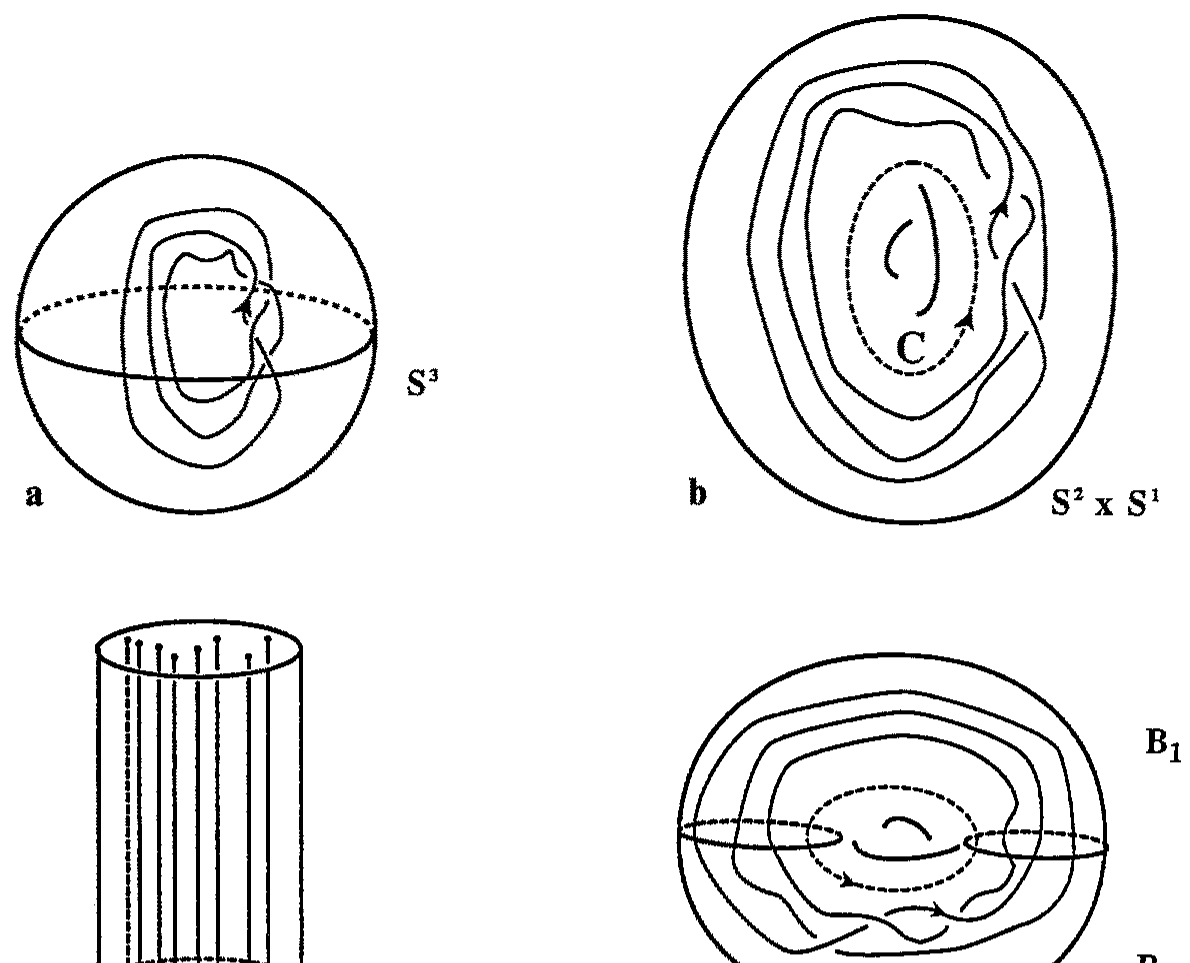
\includegraphics[width=0.82\linewidth]{figures/fig18.png}
    \caption{$S^3$ 上任一链环都可整形为 a 中的辫。把同一个辫放到 $S^2\times S^1$ 上，并对 b 中以虚线标出的圆圈 $C$ 做手术，就回到 $S^3$ 上原来的链环。若把 $S^2\times S^1$ “切开”得到 $S^2\times I$，则该辫可被“解开”（unbraided）；通过指定 $S^2$ 的一个微分同胚（据此把 c 的上下两端认同），即可还原这个辫。d 中示意辫迹之关键性质的来源：当虚线圈上存在任意威尔逊线时（这反映了手术的结果），两个辫 $B_1$ 与 $B_2$ 在 $S^2\times S^1$ 中首尾相接，无法分辨哪一个在前，因此配分函数在交换 $B_1$ 与 $B_2$ 之下不变。（原文 p.~395，Fig.~18）}
\end{figure}

我们想按照 (4.32) 的精神改写这一结果。设辫 $B$ 含 $n$ 股，构成一组表示 $\langle R\rangle$；
那么 $B$ 可以看作定义了 $n$ 个字母上的 Artin 辫群的一个元素。
辫群与带标记点的 $S^2$ 的映射类群密切相关。理由在于：若把图 18b 中的 $S^2\times S^1$ “切开”，
回到 $S^2\times I$（这相当于把图 14 中所做的事倒过来），辫就可以被“解开”。
于是，关于辫的全部信息都包含在 $S^2$ 的一个微分同胚的选取之中
（该微分同胚须保持标记点），正是用它把图 18c 的上下两端认同。
然而，这并不意味着辫群与映射类群相同：图 18b 中有 $n+1$ 股，
其中一股来自手术、并不参与辫，另外 $n$ 股才构成这个辫。
$n$ 个字母上的辫群，正是 $n+1$ 个字母上的映射类群中、固定其中一条（带标架的）股的那个子群。
利用手头的数据，可以自然地定义辫群上的若干不变迹（invariant trace），它们就是
\begin{equation}
    \tau_i(B) = Z(S^2\times S^1;\, R_i,\, B).
    \tag{4.58}
\end{equation}

% [Tutor Note: 物理图像] (4.57) 是本文全部“手术计算”的核心公式：先用 (4.27) 把 $S^3$ 上的链环
% 换成 $S^2\times S^1$ 上“辫 + 一条平行的 $R_j$ 威尔逊线”，再对 $j$ 求和。注意 $S_0{}^j$ 是
% 亏格一情形的模变换矩阵元（见 (4.27) 与 §4.3），指标位置（$S_0{}^j$ 而非 $S_{0j}$）在原文中
% 并不一致，见 (4.37)(4.42)(4.45) 用上标写法 $S_0{}^i$（$i$ 为哑指标）、(4.43)(4.46) 用
% $S_{0,j}$、(4.39) 用 $S_{mn}$；此处照原文排印，不要自行“统一”。
%
% [Tutor Note: 术语] (4.58) 定义的 $\tau_i(B)$ 正是后来所谓的 Reshetikhin--Turaev 不变量
% （在 $R_i$ 为 $SU(2)$ 基础表示时给出 Jones 多项式）的“量子迹”。Witten 用路径积分把它定义为
% $S^2\times S^1$ 上带两类威尔逊线的配分函数；RT 则用 $R$ 矩阵与辫群表示给出纯代数构造。
% 两条路线的一致性，是本文之后 Chern--Simons 理论严格化的主要检验之一（比较 [11]、[16] 与
% Reshetikhin--Turaev 1989 的工作）。

这一结果具有“迹”的关键性质：
\begin{equation}
    \tau_i(B_1 B_2) = \tau_i(B_2 B_1),
    \tag{4.59}
\end{equation}
因为 (4.59) 两端具有相同的路径积分表示：在其中，两个辫在 $S^2\times S^1$ 中首尾相接，
如图 18d 所示。(4.58) 不仅满足 (4.59)；它实际上等于算子 $B$ 在辫群的某个表示中的迹
——这个表示由 $S^2$ 上带 $n+1$ 个电荷的物理希尔伯特空间 $\mathcal{H}$ 提供，
其中应理解为辫群作用在前 $n$ 个电荷上，而第 $(n+1)$ 个电荷固定在 $R_i$ 表示中。
“$\tau_i(B)$ 是 $B$ 在该希尔伯特空间中的迹”这一陈述，正是沿着 (4.32) 的路子得到的。
因此我们可以把 (4.57) 改写为
\begin{equation}
    Z(S^3;\, L) = \sum_j S_0{}^j\, \tau_j(B).
    \tag{4.60}
\end{equation}
这表明：$S^3$ 上的链环不变量可以写成辫迹的线性组合。这与纽结多项式最初被发现的方式非常接近。
从 Tsuchiya 与 Kanie [11]、以及 Segal [16] 的工作，再结合上面所说的一切，可以清楚地看到：
由 Chern--Simons 理论得到的辫迹，恰是 Jones 工作中最早出现的那一批辫迹。

% [Tutor Note: 含糊点] “辫迹恰是 Jones 的那一批辫迹”是全节结论，但证明被压缩成一句文献引用。
% 其逻辑链是：(i) 本文 §3–§4 已证明 2+1 维 Chern--Simons 理论的物理希尔伯特空间 = 1+1 维
% WZW 模型的共形块空间；(ii) Tsuchiya--Kanie [11] 计算了 WZW 共形块在 $S^2$ 上标记点移动时的
% 单值性，得到的是辫群表示；(iii) 该表示与 Jones 用 von Neumann 代数构造的辫群表示一致
% （Kauffman [7]、Birman--Wenzel [10] 的代数侧结果）。三步合起来才得到结论。
% 严格化这条链（尤其是 (i) 中路径积分的测度与正规化）是之后十年拓扑场论严格化的主题。
%
% [Tutor Note: 易错点] (4.58) 中 $S^2\times S^1$ 上同时放置辫与一条平行威尔逊线时，
% 两条线的相对标架（framing）是固定的：平行圈 $C$ 与辫的每一股之间没有自然标架，
% 原文在 (4.57) 之前用“lifting this braid out of $S^3$”固定了它（沿 $S^2$ 法向的竖直标架）。
% 若换一种标架，$\tau_i(B)$ 会整体乘上相位 $q^{\pm\text{常数}}$；这正是 Jones 多项式
% 需要按 writhe 修正的场论根源。

\section{对物理学的应用}

\begin{keypoints}
    \item \textbf{物理图像：}2+1 维广义协变理论（陈–西蒙斯理论）的物理希尔伯特空间，
          就是 1+1 维共形场论的共形块空间；“三维的广义协变性”是二维共形场论诸多相容性条件
          （六边形、五边形等式）的统一来源。
    \item \textbf{数学工具：}带边三维流形上的路径积分、圆盘上联络空间的辛商 $LG/G$、
          圈群的最高权表示、Segal 的几何量子化定理。
    \item \textbf{关键结论：}把圆盘 $D$ 上的陈–西蒙斯理论量子化，等价于在齐性空间 $LG/G$ 上
          做量子力学；其量子希尔伯特空间给出圈群的基本不可约最高权表示，
          从而把 $2+1$ 维与 $1+1$ 维的联系具体化。
\end{keypoints}

最后，我想就这些结果对物理学可能的影响作些评论。我们一直在探讨关于共形场论的一种三维观点，
至少对黎曼面上流代数这一重要的特殊情形是如此。有理共形场论的许多方面，
都已作为三维广义协变性的自然推论浮现出来。看来很可能，[13] 中那些奇妙的六边形与五边形等式、
以及有理共形场论的其他相容性条件，都可以这样来综合：这类理论来自三维的广义协变理论。
倘若如此，三维的广义协变性或许会成为支配二维共形场论的主要统一主题之一。
正是这类考虑促成了对 $2+1$ 维引力的研究，其结果将在别处发表 [38]。

% [Tutor Note: 背景] [38] 即 Witten, \emph{$2+1$ dimensional gravity as an exactly soluble system}
% （IAS preprint HEP-88/32，后发表于 Nucl. Phys. B311 (1988) 46）。该文把 2+1 维引力
% 写成陈–西蒙斯理论（规范群为 ISO(2,1) 或其覆盖群），从而可精确求解。
% 这里所谓“二维共形场论的相容性条件来自三维广义协变性”，在今天的语言里就是：
% 有理共形场论 = 3-2-1 维拓扑场论的边界理论（Atiyah–Segal 公理体系）。

到目前为止，我们所陈述的 $2+1$ 维广义协变性与 $1+1$ 维共形不变理论之间的基本联系是：
在 $2+1$ 维量子化得到的物理希尔伯特空间，可以解释为 $1+1$ 维中共形块的空间。
这一联系可能显得相当抽象，因此我下面就作几点评论，以使它更为具体。
从三维出发，我们被引向对拉格朗日量 (3.1) 作量子化的问题，为方便起见重抄如下：
\begin{equation}
    \mathcal{L} = \frac{k}{8\pi} \int \mathrm{d}t \int_\Sigma \varepsilon^{ij}\,
    \mathrm{Tr}\, A_i \frac{\mathrm{d}}{\mathrm{d}t} A_j .
    \tag{5.1}
\end{equation}
对此应在约束 $\varepsilon^{ij}F^a_{ij}=0$ 下作量子化，这些约束正是无穷小规范变换
\begin{equation}
    A_i \to A_i - D_i \varepsilon
    \tag{5.2}
\end{equation}
的生成元。

% [Tutor Note: (5.1) 与 (1.3) 的系数对应] (5.1) 与 §3 的 (3.1) 逐字相同，是本文正则量子化的
% 出发点。§1 把陈–西蒙斯作用量 (1.3) 写成两行：第一行
% $\mathcal{L}=\frac{k}{4\pi}\int_M\Tr(A\wedge\mathrm{d}A+\frac23A\wedge A\wedge A)$，第二行
% $\mathcal{L}=\frac{k}{8\pi}\int_M\varepsilon^{ijk}\Tr\bigl(A_i(\partial_jA_k-\partial_kA_j)
% +\frac23A_i[A_j,A_k]\bigr)$。两行恒等：由 $\varepsilon^{ijk}$ 的全反对称性，
% $\varepsilon^{ijk}\Tr(A_iA_jA_k)=\frac12\varepsilon^{ijk}\Tr(A_i[A_j,A_k])$，故第二行括号内的
% $(\partial_jA_k-\partial_kA_j)$ 与 $[A_j,A_k]$ 各贡献一个因子 2，恰好抵消其系数中的 $1/2$
% （与 (1.3) 处的批注互为印证）。因此 (5.1) 的 $k/8\pi$ 对应的是 (1.3) 的**第二行**（指标形式）；
% 核对时若直接拿第一行的 $k/4\pi$ 相减，就会误以为丢了因子 2。这里 $\varepsilon^{ij}$ 已是
% $\Sigma$ 上的二维 Levi-Civita 符号，其符号由 $\Sigma$ 的定向固定。(5.1) 读出的辛形式与
% (3.2) 的括号 $4\pi/k$ 一起，确定了 (1.3) 之后由 $k\in\mathbb{Z}$ 所固定的 $\Tr$ 归一化；
% 因此不要在未固定 $\Tr$ 约定时单独调整 (5.1) 或 (3.2) 中任何一侧的系数。

到目前为止，我们只在无边黎曼面上量子化 (5.1)；现在把这个要求放宽。
在这一更一般的情形下，量子化 (5.2) 归结为研究带边三维流形上的三维陈–西蒙斯理论，
即 $\Sigma\times\mathbb{R}^1$，其中 $\Sigma$ 是带边的黎曼面。

% [Tutor Note: 原文笔误] 上一句的“量子化 (5.2)”按上下文应为 (5.1)：待量子化的是拉格朗日量
% (5.1)，而 (5.2) 是它生成的规范变换（即约束的生成元）。译文照印刷本未改号，读者对照时以
% (5.1) 为准。
例如，设 $\Sigma$ 是一个圆盘 $D$。要在圆盘上量子化 (5.1)，就必须施加这些约束，
而它们生成规范变换 (5.2)。由于 $D$ 有边界，我们必须对 $A_i$ 与 $\varepsilon$ 选取边界条件
（对闭曲面此问题不会出现）。我们将对 $A_i$ 采用自由边界条件，但要求 $\varepsilon=0$ 于边界 $S$ 上。
（这一选择的理由是：对那些在边界上不为零的规范变换，陈–西蒙斯作用量并不保持不变。）
在这一条件下，(5.2) 中的 $\varepsilon$ 生成的是在圆盘边界上为恒等变换的规范变换群 $\hat{G}_1$。
该群的一个元素是任意连续映射 $V: D\to G$，其在 $S$ 上的限制为恒等映射。

% [Tutor Note: 术语] 原文的 $\hat{G}_1$（OCR 常误作 $G_1$）指“在边界上为恒等的规范变换群”，
% 是本文后面讨论 $LG/G$ 的关键。它与圈群 $LG$ 的关系是：$LG$ 是边界 $S$ 上的规范变换群，
% 而 $\hat{G}_1$ 是其中“可延拓到圆盘内部且在边界上为恒等”的那部分；
% 取商 $LG/\hat{G}_1$ 之后，圆盘内部的信息被消去，只剩下边界上的自由度。

现在施加约束。第一步是要求 $\varepsilon^{ij}F^a_{ij}=0$。
由于圆盘是单连通的，这意味着 $A_i = -\partial_i U\cdot U^{-1}$，其中 $U: D\to G$ 为某个映射。
$U$ 在相差
\begin{equation}
    U \to U\cdot W
    \tag{5.3}
\end{equation}
的意义下唯一确定，其中 $W\in G$ 是常元素。其次，我们必须把相差一个受限规范群 $\hat{G}_1$
元素的两个 $U$ 认同。这意味着必须施加等价关系 $U\simeq VU$，其中 $V$ 是任意在边界 $S$ 上
满足 $V=1$ 的映射。这个等价关系意味着只有 $U$ 在 $S$ 上的限制才是相关的。
该限制定义了圈群 $LG$ 的一个元素；但由于自由度 (5.3)，我们实际上应把 $U$ 看作 $LG/G$ 的元素。

几何上，我们由此得知：齐性空间 $LG/G$ 可以看成圆盘 $D$ 上 $G$ 联络的空间、
在辛微分同胚群 $\hat{G}_1$ 作用下的辛商（symplectic quotient）。

% [Tutor Note: 辛商其实含两步] 原文“$LG/G$ = 圆盘上联络空间对 $\hat{G}_1$ 的辛商”是把两步合写了：
% 第一步是解约束 $F=0$（辛商中取矩映射零集）；第二步是模去在边界上为恒等的 $\hat{G}_1$——
% 后者的作用是消去圆盘内部的自由度（$U\to VU$，$V|_S=1$，故 $U|_S$ 不变），只剩 $U$ 在边界上的
% 限制，即 $LG$ 的一个元素；最后再按 (5.3) 的常元素 $G$ 取右商，才得到 $LG/G$。因此“对
% $\hat{G}_1$ 取辛商”与“模去 $G$”是两件事，不要把商群读成 $\hat{G}_1\times G$ 或 $\hat{G}_1/G$；
% 这也解释了为什么正文先得到圈群 $LG$、再把它写成 $LG/G$。
现在我们要量子化这个理论，也就是在 $LG/G$ 上做量子力学；由 (5.1)，$LG/G$ 自然地继承了一个辛结构。
显然，$\Sigma$ 边界上的规范变换群 $LG$ 作用在 $LG/G$ 上，
因此量子希尔伯特空间至少是圈群的一个射影表示。
事实上，按照 Segal [39]，以这一辛结构量子化 $LG/G$，得到的正是圈群的基本不可约最高权表示。
这就使 $2+1$ 维与 $1+1$ 维之间的联系直接得多，
因为圈群的不可约表示正是 $1+1$ 维理论的基本构件。
到这一步已经显然：考虑带有各种边界分支的更复杂的黎曼面，
我们就能生成整个 $1+1$ 维共形场论——本质上就是通过在各种带边三维流形上
研究这个广义协变的 $2+1$ 维理论。

% [Tutor Note: 含糊点] “It is obvious at this point that…” 一句跳过了把全部二维共形场论
% 从三维理论中“生成”出来的构造。其内容后来发展为 Atiyah 的拓扑场论公理与 Segal 的
% 共形场论公理：一个 $d$ 维拓扑场论是函子 $\mathrm{Cob}_d\to\mathrm{Vect}$，
% 于是“在带边三维流形上取值”= 对边界黎曼面赋以共形块空间，“沿边界粘合”= 共形块的配对。
% 原文此处的“obvious”只在如下意义下成立：把每个边界分支都看作带标记点的黎曼面，
% 逐个粘合即得。需要补的细节（模空间、反常、标记点的融合）见 Segal [16]、[39] 与
% Moore--Seiberg [13]。
%
% [Tutor Note: 易错点] “辛微分同胚群 $\hat{G}_1$”这一说法要小心：$\hat{G}_1$ 并不是
% $D$ 的微分同胚群，而是“在边界上为恒等的规范变换群”，它通过保持辛形式 (5.1) 而作用
% （因此称“辛”）；辛商是 Marsden--Weinstein 商 $LG/G$。把 $\hat{G}_1$ 误读为圆盘的
% diffeomorphism 群，会与 §3 中的“广义协变性”混淆——本文的广义协变性来自拉格朗日量不含度规，
% 与这里的辛商是两件不同的事。
%
% [Tutor Note: 物理图像] 本节的结论（$LG/G$ 的量子化 = 圈群最高权表示）是本文与二维共形场论
% 的接口。它解释了为什么 Jones 多项式的变量 $q=e^{2\pi i/(k+2)}$：$k$ 是 $LG$ 的能级，
% 而 $q$ 是最高权表示的特征标参数（$k+2$ 中的 2 来自 $SU(2)$ 的二次 Casimir 平移）。
% 这也解释了 Jones 多项式为何是 $q$ 的 Laurent 多项式、以及为什么要在 $q$ 为根单位时取极限。

\textbf{致谢（Acknowledgements）。}本工作源于这样一个认识：Segal 所描述的共形场论的某些结果，
可以通过考虑一个以陈–西蒙斯作用量为作用量的规范理论而获得三维解释。
我感谢 Segal 解释他的结果，感谢 M. Atiyah 使我对 Jones 多项式产生兴趣并给我以教益。
V.~F.~R. Jones 与 L. Kauffman、以及 IAMP 大会的其他与会者提出了许多相关问题。
最后，我必须感谢 S. Deser 与 D.~J. Gross 指出 Polyakov 的论文，
感谢 G. Moore 与 N. Seiberg 解释他们的工作，感谢 IAMP 大会组织者的盛情接待。


% =============================================================================
%  s10-references.tex —— 参考文献（原文 PDF p.47 末–p.49；印刷页 397–399）
%  照原文顺序与编号排印，条目文字保持原文（英文），未作增补或删改。
% =============================================================================
\section*{参考文献}
\markboth{参考文献}{}
\addcontentsline{toc}{section}{参考文献}

\begingroup
\small
\setlength{\parindent}{0pt}
\setlength{\itemsep}{2pt}
\begin{enumerate}[label={[\arabic*]}, leftmargin=2.4em, labelsep=0.5em, align=left]
    \item Atiyah, M.~F.: New invariants of three and four dimensional manifolds.
          In: The mathematical heritage of Hermann Weyl. Proc.\ Symp.\ Pure Math., vol.~48.
          Wells, R. (ed.). Providence, RI: American Mathematical Society 1988, pp.~285--299
    \item Donaldson, S.: An application of gauge theory to the topology of four manifolds.
          J.\ Diff.\ Geom.\ \textbf{18}, 269 (1983); Polynomial invariants for smooth
          four-manifolds. Oxford preprint
    \item Floer, A.: An instanton invariant for three manifolds. Courant Institute preprint (1987);
          Morse theory for fixed points of symplectic diffeomorphisms. Bull.\ AMS \textbf{16},
          279 (1987)
    \item Witten, E.: Topological quantum field theory. Commun.\ Math.\ Phys.\ \textbf{117},
          353 (1988)
    \item Jones, V.~F.~R.: Index for subfactors. Invent.\ Math.\ \textbf{72}, 1 (1983);
          A polynomial invariant for links via von Neumann algebras. Bull.\ AMS \textbf{12},
          103 (1985); Hecke algebra representations of braid groups and link polynomials.
          Ann.\ Math.\ \textbf{126}, 335 (1987)
    \item Freyd, P., Yetter, D., Hoste, J., Lickorish, W.~B.~R., Millett, K., Ocneanu, A.:
          A new polynomial invariant of knots and links. Bull.\ AMS \textbf{12}, 239 (1985)
    \item Kauffman, L.: State models and the Jones polynomial. Topology \textbf{26}, 395 (1987);
          Statistical mechanists and the Jones polynomial, to appear in the Proceedings of the
          July, 1986, conference on Artin's braid group, Santa Cruz, California;
          An invariant of regular isotopy, preprint
    \item Turaev, V.~G.: The Yang--Baxter equation and invariants of links.
          LOMI preprint E-3-87; Inv.\ Math.\ \textbf{92}, 527 (1988)
    \item Przytycki, J.~H., Traczyk, P.: Invariants of links of Conway type.
          Kobe J.\ Math.\ \textbf{4}, 115 (1988)
    \item Birman, J.: On the Jones polynomial of closed 3-braids. Invent.\ Math.\ \textbf{81},
          287 (1985); Birman, J., Wenzl, H.: Link polynomials and a new algebra, preprint
    \item Tsuchiya, A., Kanie, Y.: In: Conformal field theory and solvable lattice models.
          Adv.\ Stud.\ Pure Math.\ \textbf{16}, 297 (1988); Lett.\ Math.\ Phys.\ \textbf{13},
          303 (1987)
    \item Verlinde, E.: Fusion rules and modular transformations in $2d$ conformal field theory.
          Nucl.\ Phys.\ \textbf{B300}, 360 (1988)
    \item Moore, G., Seiberg, N.: Polynomial equations for rational conformal field theories.
          To appear in Phys.\ Lett.\ B; Naturality in conformal field theory. To appear in
          Nucl.\ Phys.\ B; Classical and quantum conformal field theory. IAS preprint HEP-88/35
    \item Schroer, B.: Nucl.\ Phys.\ \textbf{295}, 4 (1988); K.-H. Rehren, Schroer, B.:
          Einstein causality and Artin braids. FU preprint (1987)
    \item Fr\"ohlich, J.: Statistics of fields, the Yang--Baxter equation, and the theory of
          links and knots. 1987 Carg\`ese lectures, to appear in Nonperturbative quantum field
          theory. New York: Plenum Press
    \item Segal, G.: Conformal field theory. Oxford preprint; and lecture at the IAMP Congress,
          Swansea, July, 1988
    \item Gromov, M.: Pseudo-holomorphic curves in symplectic manifolds.
          Invent.\ Math.\ \textbf{82}, 307 (1985)
    \item Schwarz, A.: The partition function of degenerate quadratic functional and
          Ray--Singer invariants. Lett.\ Math.\ Phys.\ \textbf{2}, 247 (1978)
    \item Sch\"onfeld, J.: A mass term for three dimensional gauge fields.
          Nucl.\ Phys.\ \textbf{B185}, 157 (1981)
    \item Jackiw, R., Templeton, S.: How superrenormalizable theories cure their infrared
          divergences. Phys.\ Rev.\ \textbf{D23}, 2291 (1981)
    \item Deser, S., Jackiw, R., Templeton, S.: Three dimensional massive gauge theories.
          Phys.\ Rev.\ Lett.\ \textbf{48}, 975 (1983); Topologically massive gauge theory.
          Ann.\ Phys.\ (NY) \textbf{140}, 372 (1984)
    \item Zuckerman, G.: Action principles and global geometry. In: The proceedings of the
          1986 San Diego Summer Workshop, Yau, S.-T. (ed.)
    \item Polyakov, A.~M.: Fermi--Bose transmutations induced by gauge fields.
          Mod.\ Phys.\ Lett.\ \textbf{A3}, 325 (1988)
    \item Hagen, C.~R.: Ann.\ Phys.\ \textbf{157}, 342 (1984)
    \item Arovas, D., Schrieffer, R., Wilczek, F., Zee, A.: Statistical mechanics of anyons.
          Nucl.\ Phys.\ \textbf{B251 [FS 13]}, 117 (1985)
    \item Witten, E.: Non-Abelian bosonization in two dimensions. Commun.\ Math.\ Phys.\
          \textbf{92}, 455 (1984)
    \item Ray, D., Singer, I.: Adv.\ Math.\ \textbf{7}, 145 (1971); Ann.\ Math.\ \textbf{98},
          154 (1973)
    \item Deser, S., Jackiw, R., Templeton, S.: In [21]; Affleck, I., Harvey, J., Witten, E.:
          Nucl.\ Phys.\ \textbf{B206}, 413 (1982); Redlich, A.~N.: Gauge invariance and parity
          conservation of three-dimensional fermions. Phys.\ Rev.\ Lett.\ \textbf{52}, 18 (1984);
          Alvarez-Gaum\'e, L., Witten, E.: Gravitational anomalies. Nucl.\ Phys.\ \textbf{B234},
          269 (1983); Alvarez-Gaum\'e, L., Della Pietra, S., Moore, G.: Anomalies and odd
          dimensions. Ann.\ Phys.\ (NY) \textbf{163}, 288 (1985); Atiyah, M.~F.: A note on the
          eta invariant (unpublished); Singer, I.~M.: Families of Dirac operators with
          applications to Physics. Ast\'erisque, 1985, p.~323
    \item Atiyah, M.~F., Patodi, V., Singer, I.: Math.\ Proc.\ Camb.\ Phil.\ Soc.\ \textbf{77},
          43 (1975); \textbf{78}, 405 (1975); \textbf{79}, 71 (1976)
    \item Wilczek, F., Zee, A.: Linking numbers, spin, and statistics of solitons.
          Phys.\ Rev.\ Lett.\ \textbf{51}, 2250 (1983)
    \item Friedan, D., Shenker, S.: Nucl.\ Phys.\ \textbf{B281}, 509 (1987)
    \item Belavin, A., Polyakov, A.~M., Zamolodchikov, A.: Nucl.\ Phys.\ B (1984)
    \item Atiyah, M.~F., Bott, R.: The Yang--Mills equations over Riemann surfaces.
          Phil.\ Trans.\ R.\ Soc.\ Lond.\ \textbf{A308}, 523 (1982)
    \item Quillen, D.: Determinants of Cauchy--Riemann operators over a Riemann surface.
          Funct.\ Anal.\ Appl.\ \textbf{19}, 31 (1986)
    \item Drinfeld, V.: Quantum groups. In: The Proceedings of the International Congress of
          Mathematicians, Berkeley 1986, Vol.~1, pp.~798--820
    \item Gepner, D., Witten, E.: String theory on group manifolds. Nucl.\ Phys.\ \textbf{B278},
          493 (1986)
    \item Kac, V.~G.: Infinite dimensional Lie algebras. Cambridge: Cambridge University Press
          (1985); Kac, V.~G., Peterson, D.~H.: Adv.\ Math.\ \textbf{53}, 125 (1984);
          Kac, V.~G., Wakimoto, M.: Adv.\ Math.\ \textbf{70}, 156 (1988)
    \item Witten, E.: $2+1$ dimensional gravity as an exactly soluble system.
          IAS preprint HEP-88/32
    \item Segal, G.: Unitary representation of some infinite dimensional groups.
          Commun.\ Math.\ Phys.\ \textbf{80}, 301 (1981)
\end{enumerate}
\endgroup

\vspace{1.2em}
\begin{center}
\small
（编辑部：Communicated by A.~Jaffe；收稿 1988 年 9 月 12 日，修改稿 1988 年 9 月 27 日）
\end{center}


\end{document}